\chapter{No Linealidad Geométrica}\label{cap2GNA}

En este capítulo se presentan algunos conceptos centrales del análisis de estructuras que exhiben no linealidad geométrica. Se hará foco en estructuras discretas, es decir no se hará énfasis en cuerpos continuos.

En la primer sección se presenta el Principio de Mínima Energía Potencial Total como herramienta para hallar las ecuaciones de equilibrio de estructuras elásticas y estudiar la estabilidad de dichas estructuras, en la hipótesis de grandes desplazamientos. %
%
A continuación se presenta el Principio de los Trabajos Virtuales como una herramienta alternativa, y más general que la anterior, para determinar las ecuaciones de equilibrio de estructuras. %
% 
Posteriormente se introducen diferentes medidas de deformación no lineal como función de desplazamientos, aplicadas a miembros de tipo biela. %
%
Habiendo cubierto los conceptos anteriores, se introduce una formulación de elementos finitos para bielas elásticas lineales. %
%
Dicha formulación permite analizar estructuras reticuladas sometidas a grandes desplazamientos y rotaciones con pequeñas deformaciones unitarias. %
%
Finalmente, se aplican los conceptos vistos para describir métodos de análisis de estabilidad estructural en reticulados.




\section{Principio de Mínima Energía Potencial Total}

En esta sección se introduce el Principio de Mínima Energía Potencial Total (PMEPT), el cual permite determinar las ecuaciones de equilibrio y estudiar la estabilidad de sistemas estructurales conservativos no lineales\footnote{Como complemento a esta sección se recomienda ver la presentación, del Profesor M. A. Wadee del \textit{Imperial College London}, titulada \textit{Sandwiches, snakes and stays: interacting with instabilities}, disponible en: \href{https://youtu.be/NSFqwxW7gRo}{https://youtu.be/NSFqwxW7gRo} (último acceso mayo de 2021).}
%
También es posible profundizar en el análisis, mediante enfoques energéticos, de la estabilidad elástica de estructuras siguiendo los libros \citep{thompson1973general,Crisfield1997} y en forma un poco menos específica con el libro \citep{timoshenko2012theory}.

\subsection{Definición de Energía Potencial Total}\label{TPE_Def}

Tal como fue indicado, se abordará el estudio de sistemas estructurales discretos en los cuales se puede definir completamente la configuración del sistema mediante un número $(n)$ de coordenadas generalizadas ($\bfq=(q_1,q_2,...,q_n)^T\in\mathbb{R}^n$).

Un sistema estructural conservativo que se encuentra en la configuración dada por $\bfq$ tendrá una energía potencial total $V(\bfq)$ definida como: %
%
\begin{equation}
V(\bfq) = U(\bfq) - W_E(\bfq),
\end{equation}
%
donde $U(\bfq)$ es la energía elástica interna del sistema en la configuración dada por $\bfq$ y $W_E(\bfq)$ es el trabajo realizado por las fuerzas externas conservativas aplicadas sobre el sistema desde una configuración de referencia arbitraria hasta la configuración $\bfq$.

Un ejemplo sencillo mediante el cual se pueden fijar estos conceptos es el de un sistema de una masa puntal ($m$) y un resorte elástico lineal de constante ($K$) sujeto a la acción externa de la gravedad ($g$), como el que se muestra en la Figura \ref{fig:fig7}.

\begin{figure}[htb]
	\centering
   \def\svgwidth{0.3\textwidth}
\input{../fig/massSpring.pdf_tex}
	\caption{Esquema de sistema Masa-Resorte.}
	\label{fig:fig7}
\end{figure}

Se asume una configuración (no necesariamente de equilibrio) en la cual la masa se desplaza $q$ respecto de la posición neutra del resorte. En dicha configuración, el resorte se encuentra comprimido, con una cierta energía elástica interna almacenada y la gravedad realizó un cierto trabajo,

\begin{equation}
U(q)=\frac{Kq^2}{2}+C_1 \quad \text{y} \quad W_E(q)=mgq + C_2,
\end{equation}
%
respectivamente. %
%
Las constantes $C_1$ y $C_2$ corresponden a las referencias que se tomen tanto para definir energía elástica interna como trabajo de fuerzas conservativas externas. Como se verá más adelante, estas constantes son intrascendentes para estudiar el equilibrio y la estabilidad y pueden ser consideradas nulas por conveniencia.

La expresión de energía elástica interna del resorte se puede obtener considerando el trabajo que se debe realizar sobre el resorte para llevarlo a una configuración comprimida (o extendida), en particular evaluando la siguiente integral:
%
\begin{equation}
U(q) = \int_{q_1}^{q} F(u)\text{ }\dif u = \int_{q_1}^{q} Ku\text{ }\dif u = \frac{Kq^2}{2} + C_1.
\end{equation}

Dicha integral es la definición de un componente elástico. Notar que uno podría eventualmente utilizar una expresión no lineal para $F(u)$, con lo cual se estaría considerando un resorte elástico pero no lineal.

A partir de lo anterior, el ejemplo de la masa y el resorte sometido a la acción de la gravedad resulta tener la siguiente expresión para la energía potencial total:
%
\begin{equation}
	V(q) = \frac{Kq^2}{2} - mgq.
\end{equation}







\subsection{Equilibrio y Estabilidad}\label{TPE_EQ_STB}

La definición de Energía Potencial Total de la sección anterior permite expresar el equilibrio y la estabilidad de los sistemas estructurales de manera extremadamente sencilla.

\cajaconcepto{Axioma 1}{$\hat{\bfq}$ es de Equilibrio $\Leftrightarrow$ $V(\bfq)$ es estacionaria en $\hat{\bfq}$}

%\begin{axioma}
%	$\hat{\bfq}$ es de Equilibrio $\Leftrightarrow$ $V(\bfq)$ es estacionaria en $\hat{\bfq}$
%\end{axioma}

Se puede mostrar que la condición de equilibrio estático correspondiente a esta definición es equivalente a la que se obtiene mediante la segunda ley de Newton. %
%
La ventaja de formular el equilibrio mediante el Principio de Mínima Energía Potencial Total es que dicho procedimiento es significativamente más sencillo y sistemático que el de Newton. Sin embargo, se puede argumentar que se pierde cierta cuota de intuición con lo cual la segunda ley de Newton sigue teniendo un importante valor.

\cajaconcepto{Axioma 2}{	$\hat{\bfq}$ es Estable $\Leftrightarrow$ $V(\bfq)$ es tiene un mínimo relativo estricto en $\hat{\bfq}$}

La definición de estabilidad del equilibrio estático dada por la expresión anterior es particularmente simple de estudiar, especialmente si se compara contra la alternativa de estudiar la estabilidad de las soluciones de las ecuaciones dinámicas del sistema frente a perturbaciones respecto de los equilibrios estáticos.

Si la función $V(\bfq)$ es suficientemente suave, las condiciones de equilibrio y estabilidad pueden ser expresadas usando derivadas parciales de $V(\bfq)$:
%
\begin{itemize}
	\item \textbf{Equilibrio} $\Leftrightarrow$ $\left. \dfrac{\partial V}{\partial \bfq}  \right|_{\hat{\bfq}} = 0$	
	%
	\item \textbf{Estabilidad} $\Leftarrow$ $\left. \text{\bfH}_V  \right|_{\hat{\bfq}}$ es definida positiva.
\end{itemize}
%
donde $\bfH_V$ es la matriz Hessiana de derivadas parciales segundas de $V(\bfq)$. %
%
Una matriz $\bfA$ es definida positiva por definición si: $\forall \bfu\neq 0 \in \mathbb{R}^N$ se cumple $\bfu^T \bfA \bfu > 0$. La definición de matriz definida positiva en el caso de matrices reales diagonalizables es equivalente a que todos los valores propios sean positivos.

En el ejemplo del sistema masa-resorte, se puede ver que la condición de equilibrio resulta en:
%
\begin{equation}
	\dfrac{dV(q)}{dq}=Kq - mg = 0,
\end{equation}
%
lo cual resulta en la posición de equilibrio esperada para el sistema. Adicionalmente, se puede ver que $\dfrac{d^2V(q)}{dq^2}=K>0$, a partir de lo cual el axioma de estabilidad garantiza que el equilibrio $\hat{q}=mg/K$ es estable como era de esperar.

\subsubsection{Equilibrio y estabilidad en sistemas de un grado de libertad}

La deducción de la condición de estabilidad para una $V(q)$ diferenciable en un grado de libertad ($q\in\mathbb{R}$) se presenta a continuación.

Haciendo un desarrollo de Taylor de $V(q)$ en el punto $\hat{q}$, se tiene un entorno de radio $\epsilon$ de $\hat{q}$ tal que $\forall \delta < \epsilon$:
%
\begin{equation}\label{Estabilidad}
V(\hat{q}+\delta)=V(\hat{q})+\left.V'(q)\right|_{\hat{q}} \delta +\frac{1}{2!} \left.V''(q)\right|_{\hat{q}} \delta^2 +\frac{1}{3!} \left.V'''(q)\right|_{\hat{q}} \delta^3 +...
\end{equation}

La condición de mínimo relativo estricto de $V(q)$ en $\hat{q}$ corresponde a que exista un entorno de $\hat{q}$ tal que $\forall \delta$ se cumpla:
%
\begin{equation}\label{CondEstab}
V(\hat{q}+\delta) - V(\hat{q}) > 0.
\end{equation}

Despejando de la Ecuación~\eqref{Estabilidad}, se obtiene:
%
\begin{equation}
V(\hat{q}+\delta) - V(\hat{q}) = \left. V'(q)\right|_{\hat{q}}\delta + \frac{1}{2!} \left.V''(q)\right|_{\hat{q}} \delta^2 +\frac{1}{3!} \left.V'''(q)\right|_{\hat{q}} \delta^3 +... 
\end{equation}

Dado que se considera una configuración de equilibrio, se debe verificar que $\left. V'(q)\right|_{\hat{q}}=0$. %
%
De esa manera se obtiene la siguiente igualdad:
%
\begin{equation}
V(\hat{q}+\delta) - V(\hat{q}) =	\frac{1}{2!} \left.V''(q)\right|_{\hat{q}} \delta^2 +\frac{1}{3!} \left.V'''(q)\right|_{\hat{q}} \delta^3 +...  \quad  \forall \delta < \epsilon
\end{equation}
%
con lo cual, se observa que si $\left.V''(q)\right|_{\hat{q}}>0$ (y $\delta$ es pequeño) entonces se satisface la desigualdad de la Ecuación~\eqref{CondEstab} y por lo tanto $\hat{q}$ es un punto estable.


Notar que podría ocurrir que $\left.V''(q)\right|_{\hat{q}}=0$ y se podría tener estabilidad si $\left.V'''(q)\right|_{\hat{q}}=0$ y $\left.V^{(4)}(q)\right|_{\hat{q}}>0$. Con lo cual, estabilidad no necesariamente implica derivada segunda de $V$ positiva. De todas formas, si ocurre lo anterior diremos que el sistema es débilmente estable.

\subsubsection{Clasificación de curvas de carga-desplazamiento}

Las curvas de carga-desplazamiento pueden ser clasificadas a partir del estudio de la estabilidad de los equilibrios de los puntos que las integran. %
%
Partiendo de una estructura sin carga aplicada ($\lambda=0$) e incrementando el factor de carga gradualmente, se puede obtener un primer punto de equilibrio sobre la curva de carga-desplazamiento para el cual $V''(q)=0$. %
%
Este punto es llamado \textit{Punto Crítico}: $C=(P^c,Q^c)$. %
%
En la Figura~\ref{fig:fig8} se presenta un ejemplo de curva carga-desplazamiento en la cual, para cada nivel de carga, se esquematiza la energía potencial total (ver \citep{thompson1973general} por otros ejemplos de este tipo de diagramas). %
%
En cuanto a las curvas de carga-desplazamiento, las lineas sólidas muestran equilibrios estables mientras que las punteadas muestran equilibrios inestables. Se debe notar la coincidencia de mínimos (máximos) de la Energía Potencial Total con puntos de equilibrio estable (inestable).

\begin{figure}[htb]
	\centering
\def\svgwidth{0.8\textwidth}
\input{../fig/BifSymStab.pdf_tex}
	\caption{Curva carga-desplazamiento de sistema con bifurcación simétrica estable.}
	\label{fig:fig8}
\end{figure}

\subsection{Clasificación de Puntos Críticos}

En esta sección se presenta una clasificación de puntos críticos a través de un conjunto de sistemas estructurales formados por barras rígidas unidas por articulaciones y resortes elásticos lineales (de desplazamiento y/o de giro). %
%
%
Para cada estructura y sistema de cargas se muestran las curvas de carga-desplazamiento para la estructura sin imperfecciones (curva que parte del origen en color negro) y con imperfecciones geométricas (curvas que presentan un desplazamiento para carga nula en color azul). %
%
Los tramos de trazo continuo representan equilibrios estables mientras que los tramos discontinuos puntos de algún tipo de inestabilidad como se verá más adelante.


\subsubsection{Punto Límite}\label{MisesTruss}

Un punto límite corresponde a una situación en la cual la estructura alcanza un punto de equilibrio inestable para el cual se produce un salto a otro equilibrio estable de manera dinámica (en inglés ''\textit{Snap-through}"). %
%
En la Figura~\ref{fig:ptolimitea} se puede observar una estructura con este comportamiento. %
%
La estructura es simétrica respecto al eje vertical y el resorte horizontal tiene comportamiento lineal. %
%
Las barras en la configuración de referencia forman un ángulo $\alpha$ con la horizontal, mientras que $\theta$ indica el ángulo correspondiente a las barras en la posición deformada.

\begin{figure}[htb]
	\centering
	\subfloat[Esquema de estructura.]{
\def\svgwidth{0.55\textwidth}
\input{../fig/limitpointink.pdf_tex}
\label{fig:ptolimitea}}
%
\subfloat[Curva carga-desplazamiento.]{
\def\svgwidth{0.55\textwidth}
\input{../fig/limitpoint.pdf_tex}
\label{fig:ptolimiteb}}
	\caption{Estructura con comportamiento de punto límite.}
	\label{fig:fig9}
\end{figure}


En la Figura~\ref{fig:ptolimiteb} se muestra la curva carga desplazamiento correspondiente. %
%
El tramo punteado indica puntos de equilibrio inestable.  %
%
La estructura presenta un punto límite en el punto indicado en el gráfico. %
%
El comportamiento de estas estructuras no es sensible a imperfecciones.
%

\subsubsection{Bifurcación Simétrica Estable}

Una bifurcación simétrica estable corresponde a una situación en la cual una estructura alcanza un punto crítico y a partir de ese punto, su curva de carga-desplazamiento se bifurca en varias ramas: una inestable y otras dos estables. %

El pandeo de columnas elásticas pertenece a esta categoría. %
%
En la Figura~\ref{fig:bifsima} se puede ver una versión discreta de ese tipo de estructura. En estos casos, al alcanzarse la bifurcación las estructuras logran mantener la carga aunque sea con grandes deformaciones (ej. regla elástica en compresión). %
%
En la Figura \ref{fig:bifsimb} se muestra la curva carga-desplazamiento correspondiente. %
%
Notar que estas estructuras tampoco son sensibles a imperfecciones, siempre y cuando el comportamiento permanezca elástico.

\begin{figure}[htb]
	\centering
		\subfloat[Esquema de estructura.]{
\def\svgwidth{0.25\textwidth}
\input{../fig/SymStable_estru.pdf_tex}
			\label{fig:bifsima}}
\hspace{0.05\textwidth}
		\subfloat[Curva carga-desplazamiento.]{
			\def\svgwidth{0.6\textwidth}
			\input{../fig/SymStable_curv.pdf_tex}
			\label{fig:bifsimb}}
	\caption{Estructura con comportamiento de bifurcación simétrica estable.}
	\label{fig:fig10}
\end{figure}



\subsubsection{Bifurcación Simétrica Inestable}

Este tipo de comportamiento se corresponde al de estructuras y cargas tales que, al alcanzarse la carga crítica, la curva de carga-desplazamiento se divide en varias ramas, todas inestables. %
%
La rama inicial (fundamental) es la única estable. %

Las cáscaras esbeltas sometidas a compresión meridional muestran este tipo de inestabilidad, ya que al alcanzar el punto de bifurcación pierden la capacidad de soportar la carga (ej. lata de aluminio en compresión). %
%
En la Figura \ref{fig:bifsimuna} se muestra una estructura discreta que exhibe este comportamiento, la configuración de la estructura sin carga aplicada es representada por líneas punteada ($\theta = 0$) mientras que en líneas sólidas se muestra la configuración deformada.

\begin{figure}[htb]
	\centering
		\centering
		\subfloat[Esquema de estructura.]{
\def\svgwidth{0.27\textwidth}
\input{../fig/SymUnstable_estru.pdf_tex}
			\label{fig:bifsimuna}}
		%
	\hspace{0.05\textwidth}
		\centering
		\subfloat[Curva carga-desplazamiento.]{
\def\svgwidth{0.62\textwidth}
\input{../fig/SymUnstable_curv.pdf_tex}
			\label{fig:bifsimunb}}
	\caption{Estructura con comportamiento de bifurcación simétrica inestable.}
	\label{fig:fig11}
\end{figure}

En la Figura~\ref{fig:bifsimunb} se muestran las curvas carga-desplazamiento, donde se recuerda que líneas sólidas corresponden a curvas con puntos de equilibrio estable y lìneas punteadas corresponden a puntos de equilibrio inestable. %

En el gráfico se observa que el comportamiento de estas estructuras es considerablemente sensible a imperfecciones. En general, la carga máxima soportada por la estructura decrece al considerar imperfecciones geométricas. %
%
El resultado observado en este ejemplo pone en evidencia la importancia de este tipo de análisis en estructuras como cáscaras.
%

\subsubsection{Bifurcación Asimétrica}

Este tipo de comportamiento corresponde a situaciones en las cuales la estructura alcanza una configuración de equilibrio inestable en la cual la curva de carga-desplazamiento se divide en varias ramas: dos ramas inestables y una estable. %
%
En la Figura~\ref{fig:bifasima} se muestra otro ejemplo de estructura con este comportamiento. %
%
En la Figura~\ref{fig:bifasimb} se muestran las curvas carga-desplazamiento.

\begin{figure}[htb]
	\centering
		\subfloat[Esquema de estructura.]{
\def\svgwidth{0.42\textwidth}
\input{../fig/Asym_estru.pdf_tex}
			\label{fig:bifasima}}
		%
	\hspace{0.003\textwidth}
		\subfloat[Curva carga-desplazamiento.]{
\def\svgwidth{0.54\textwidth}
\input{../fig/Asym_curv.pdf_tex}
			\label{fig:bifasimb}}
	\caption{Ejemplo de estructura con comportamiento de bifurcación asimétrica.}
	\label{fig:fig12}
\end{figure}

Considerando perturbaciones o imperfecciones hacia un lado la estructura se sigue una rama estable, mientras que con perturbaciones hacia el otro lado se sigue una rama inestable, con lo cual, se clasifica como inestable en general. %
%
Consecuentemente la estructura es considerada como sensible a imperfecciones. %
El pórtico in-desplazable conocido como \textit{Roorda Frame} presenta un comportamiento de tipo bifurcación asimétrica \citep{thompson1973general}.


\subsection{Ejemplo de Análisis de Equilibrio y Estabilidad}

En lo que sigue se realiza el análisis, a modo de ejemplo, de la estructura correspondiente a una versión discreta de una viga-columna en compresión, la cual exhibe una bifurcación simétrica estable. 

%\begin{figure}[htb]
%	\centering
%	\includegraphics[width=.25\linewidth]{sourcesJBBG/VigaColumna}
%	\caption{Estructura Discreta tipo Viga-Columna en Compresión.}
%	\label{fig:fig12a}
%\end{figure}

La configuración de la estructura queda totalmente definida por el ángulo que forma la barra rígida superior con la vertical ($\theta$). Tomaremos como configuración de referencia para la energía interna y el trabajo externo la situación de: $\theta=0$.

El giro relativo ($\varphi$) entre las dos barras conectadas mediante el resorte de giro es igual a: $\varphi = 2\theta$. El descenso ($\Delta$) del punto de aplicación de carga respecto de la configuración de referencia es:
%
\begin{equation}\label{SimBif_NL}
\Delta = 2L(1-\cos(\theta))
\end{equation}


A partir de esto, se puede escribir la energía elástica interna y el trabajo de la fuerza aplicada en función de $\theta$ como:
%
\begin{equation}
U(\theta)=\frac{1}{2}K (2\theta)^2 \quad \text{ y }  \quad W_E(\theta) = 2P L(1-\cos(\theta)),
\end{equation}
respectivamente. La energía potencial total es, por lo tanto, igual a:
%
\begin{equation}
V(\theta) = \frac{1}{2}4K \theta^2 - 2PL(1-\cos(\theta)).
\end{equation}

La ecuación de equilibrio queda definida, mediante la condición $V'(\theta)=0$, como:
%
\begin{equation}\label{SymBif_Eq}
4K\theta - 2PL\sin(\theta)=0.
\end{equation}
%
Las soluciones de esta ecuación no lineal cumplen alguna de las siguientes condiciones:
%
\begin{itemize}
	\item Rama F: $\theta=0 \qquad \forall P\in\mathbb{R}$
	\item Rama E: $P= 2K\theta /(L\sin(\theta))$ con: $\theta\in(-\pi,\pi)\setminus0$.
\end{itemize}

La rama de la solución hallada que pasa por el origen: ($P=0$, $\theta=0$) es llamada la \textit{rama fundamental} (Rama F).

Se procede a estudiar la estabilidad de los equilibrios hallados. En primer lugar se analiza la estabilidad de la rama fundamental. Para ello primero se debe calcular la derivada segunda de la energía potencial total: $V''(\theta)$
%
\begin{equation}
V''(\theta)=4K - 2PL\cos(\theta),
\end{equation}
%
luego, evaluando dicha función en la rama fundamental se obtiene:
%
\begin{equation}
\left.V''(\theta)\right|_F=4K - 2PL.
\end{equation}

Se puede observar que $P^C=2K/L$ es el nivel de carga del punto crítico, ya que la derivada segunda se anula por primera vez para esa carga. %
%
En dicho nivel de carga la rama fundamental se bifurca, es decir que el equilibrio en $\theta=0$ es estable para cargas menores a $P^C$ e inestable para cargas mayores a $P^C$.

Para estudiar la estabilidad de las ramas secundarias se evalúa la derivada segunda de $V(\theta)$ obteniendo:
%
\begin{equation}\label{ec16}
  \left.V''(\theta)\right|_E=4K\left(1-\frac{\theta}{\tan(\theta)}\right)>0.
\end{equation}

A partir de la Ecuación~\eqref{ec16} se comprueba que la Rama E $(\theta\neq0)$ es estable.

\cajaactividad{
%
Repetir el análisis anterior considerando la aproximación: $\cos(\theta)\simeq 1 - \theta^2 / 2$ en la Ecuación~\eqref{SimBif_NL}. %
%
Mostrar que es posible identificar el punto crítico y la simetría de la bifurcación. %
%
Verificar que no es posible establecer si el equilibrio de las ramas es estable o inestable y proponer una mejora de la aproximación para lograr esto.}


\section{Principio de los Trabajos Virtuales}

En esta sección se introduce el Principio de los Trabajos Virtuales (PTV), con el objetivo de generar intuición sobre su fundamento y validez para el análisis de estructuras. %
%
El PTV es una formulación variacional del equilibrio estático, esto significa que se plantea la condición de equilibrio como una relación que debe satisfacerse para perturbaciones virtuales arbitrarias del sistema estructural. %
%
Esta formulación del equilibrio es usualmente llamada forma débil y es frecuentemente utilizada para el desarrollo formal de métodos numéricos para análisis de estructuras \citep{Hughes1987a}.

Se presentarán ejemplos triviales didácticos de aplicación del PTV para determinar las ecuaciones de equilibrio estático. Se introducen luego ejemplos de aplicación del PTV de mayor interés práctico en los que se incluyen componentes deformables. Adicionalmente, se mostrará la relación entre el equilibrio calculado mediante el Principio de Mínima Energía Potencial Total y el determinado mediante el PTV. Finalmente, se presenta la formulación del PTV para elementos de tipo biela (miembros puramente axiales) necesaria para la formulación sistemática del Método de Elementos Finitos.


Para la presentación de los conceptos de esta sección se adoptó un abordaje similar al de \citep{mcguire1999matrix}, sin embargo se puede encontrar otros desarrollos en libros como \citep{Reddy2002b} o \citep{Bathe2014}.




\subsection{PTV para Partículas y Sistemas de Partículas}

En lo que sigue se busca mostrar la equivalencia entre el enunciado del equilibrio estático de una partícula mediante la Segunda Ley de Newton y el Principio de los Trabajos Virtuales (PTV). En primer lugar se enuncia el PTV y luego se demostrará su equivalencia con Newton.

\cajaconcepto{Principio de Trabajos virtuales para una partícula}{
	Una partícula está en equilibrio estático si se cumple que: para todo desplazamiento virtual el trabajo de las fuerzas externas es nulo, es decir:
	$$
	\delta W_{\text{ext}}=0 \qquad \forall \delta \bfx.
	$$
}
%
A continuación se muestra que el equilibrio estático según la Segunda Ley de Newton implica el PTV. 

Sea una partícula sometida a un conjunto de fuerzas externas ($\bff_i$) en equilibrio estático tal como se muestra en la Figura~\ref{fig:PTVpart}. %

\begin{figure}[htb]
	\centering
\def\svgwidth{0.35\textwidth}
\input{../fig/PTVpartic.pdf_tex}
	\caption{Equilibrio de partícula sometida a fuerzas externas.}
	\label{fig:PTVpart}
\end{figure}

El equilibrio estático puede ser expresado mediante la Segunda Ley de Newton como la siguiente ecuación vectorial
%
\begin{equation}\label{ecnewt}
\sum_{i=1}^{n_f} \bff_i = 0,
\end{equation}
%
siendo $n_f$ el número de fuerzas aplicadas (en este caso $n_f=3$).

Proyectando ambos lados de la igualdad dada en (\ref{ecnewt}) según la dirección de un vector unitario cualquiera $\hat{\bfu}$ se obtiene
%
\begin{equation}\label{ecnewtscal}
\sum_{i=1}^{n_f} \hat{\bfu}^T \bff_i = 0.
\end{equation}

Se define el Desplazamiento Virtual de la partícula como $\delta \bfx$, siendo éste un pequeño desplazamiento virtual o hipotético de la partícula, el cual no afecta el sistema de fuerzas externo aplicado. En base a este desplazamiento virtual definimos el Trabajo Virtual Externo, $\delta W_{\text{ext}}$, como aquel que realizan las fuerzas externas para el desplazamiento virtual:
%
\begin{equation}\label{defdWext}
\delta W_{\text{ext}} = \sum_{i=1}^{n_f} \delta \bfx^T \bff_i.
\end{equation}

Dado que el desplazamiento virtual es arbitrario, el mismo puede ser expresado como el producto de un vector unitario con dirección arbitraria $\hat{\bfu}$ y una constante $\delta x$ pequeña arbitraria . Es decir: $\delta \bfx = \delta x \text{ }\hat{\bfu}$.

A partir de lo anterior y la definición de la Ecuación~\eqref{defdWext} se tiene que
%
\begin{equation}
\delta W_{\text{ext}} = \delta x \sum_{i=1}^{n_f} \hat{\bfu}^T \bff_i  \qquad \forall \delta x, \forall \hat{\bfu}
\end{equation}

Usando el equilibrio estático dado por Newton en la Ecuación~\eqref{ecnewtscal}, se concluye que
%
\begin{equation}\label{PTV_part}
\delta W_{\text{ext}} = 0 \qquad  \forall \delta\bfx,
\end{equation}
%
por lo que queda probado que el equilibrio de Newton implica que se cumpla el PTV para la partícula.

\cajaactividad{
	Mostrar el recíproco del resultado anterior, es decir, mostrar que el PTV implica la segunda ley de Newton.
}






\subsection{PTV para Cuerpos Rígidos}

Se propone avanzar, usando el resultado anterior, hacia el planteo del PTV para un cuerpo rígido.

La hipótesis central considerada es que el cuerpo que estudiado es rígido, por lo tanto incluso ante desplazamientos virtuales el cuerpo permanece rígido. %
%
Se ilustra la situación mediante el ejemplo de una barra rígida simplemente apoyada en sus extremos y sometida a una fuerza lateral en la mitad de su largo, ver Figura~\ref{fig:CuerpoRigido}.
%
\begin{figure}[htb]
	\centering
	\subfloat[Equilibrio de cuerpo rígido sometida a fuerzas externas.]{
\def\svgwidth{0.7\textwidth}
\input{../fig/Cuerporigido.pdf_tex}
	\label{fig:CuerpoRigido}}\\
	\subfloat[Movimiento virtual de cuerpo rígido.]{
\def\svgwidth{0.7\textwidth}
\input{../fig/PTV_CuerpoRigido.pdf_tex}
		\label{fig:PTV_CuerpoRigido}}
	\caption{PTV aplicado a equilibrio de cuerpo rígido.}
\end{figure}
%
Para poder realizar un desplazamiento virtual de la barra rígida, se cambia el apoyo deslizante derecho por una fuerza estáticamente equivalente (la reacción vertical), ver Figura \ref{fig:PTV_CuerpoRigido}. %
%
Una vez liberado ese vínculo, se puede considerar un desplazamiento virtual $\delta \bfx$ de la barra rígida. %
%
Dicho desplazamiento debe satisfacer la condición de borde en desplazamiento dada en el apoyo simple izquierdo y también la condición de cuerpo rígido de la barra. %
%
Se concluye que el desplazamiento virtual debe ser un giro rígido en torno al apoyo izquierdo.

Dado que el PTV para una partícula también se aplica a un sistema de partículas, se puede considerar el cuerpo rígido como un sistema de partículas con la propiedad que las distancias relativas entre ellas se mantienen constantes. %
%
De lo anterior se concluye que las fuerzas entre partículas no realizan trabajo virtual ya que durante el desplazamiento virtual no hay cambios en las distancias relativas entre ellas y por consiguiente no hay trabajo virtual. %
%
Por otro lado, la fuerza externa aplicada sí realiza trabajo sobre el desplazamiento virtual y lo mismo vale para la reacción derecha. A partir del razonamiento anterior y el PTV para sistemas de partículas, se tiene:
%
\begin{equation}
\delta W_{\text{ext}} = -P \text{ } \frac{\delta u}{2} + R_B \text{ } \delta u = 0 \qquad \forall \delta u
\end{equation}

Se obtiene la siguiente ecuación:
%
\begin{equation}\label{PTVRigid}
\left( -\frac{P}{2} + R_B \right) \delta u = 0 \qquad \forall \delta u,
\end{equation}
%
donde, para que el producto se anule para todo $\delta u$ se debe cumplir:
%
\begin{equation}
R_B = \frac{P}{2}.
\end{equation}

La reacción vertical del apoyo izquierdo se puede determinar mediante un procedimiento idéntico al presentado para la reacción del apoyo derecho.

En conclusión, el PTV para cuerpos rígidos tiene la misma forma que el dado para sistemas de partículas. Notar que se deben liberar vínculos de manera de poder realizar los desplazamientos virtuales necesarios para determinar las ecuaciones de equilibrio.

\cajaactividad{
	%
	Determinar todas las reacciones del ejemplo visto en esta sección, liberando todos los vínculos de apoyo al mismo tiempo y generando así un sistema de ecuaciones para determinar dichas reacciones.}

\subsection{PTV para Estructuras con Componentes Deformables} \label{sec:ptvestdef}
Dados los conceptos presentados hasta aquí, se puede pasar a estudiar el PTV aplicado a estructuras con componentes deformables. %
%
Puntualmente, se considerará como ejemplo la cercha de Von Mises, la cual fue introducida en la Sección~\ref{MisesTruss}. 

La estructura está compuesta por dos barras de largo $L$, rígidas, unidas por una articulación perfecta. El extremo libre izquierdo de las barras se soporta mediante un apoyo fijo y el extremo libre derecho mediante un apoyo deslizante. %
%
Ambos apoyos se unen con un resorte, es decir, un cuerpo deformable (ver Figura~\ref{fig:ptolimitea}). %
%
Notar que no se especifica la relación constitutiva del resorte. La estructura se somete a una carga externa vertical descendente $P$ y el ángulo que forma una de las barras inclinadas con la horizontal para $P=0$ es igual a $\alpha$. 

El paso clave para determinar el equilibrio del sistema estructural consiste en sustituir el cuerpo deformable (resorte) por un conjunto de fuerzas estáticamente equivalente y equilibrado aplicado al resto de la estructura.

Cuando la estructura está en una configuración de equilibrio, el resorte puede ser sustituido por dos fuerzas opuestas de valor $F_{\text{int}}$ aplicadas en los nodos de los extremos. %
%
De esta forma se vuelve a tener una estructura compuesta de cuerpos rígidos sometida a fuerzas externas (ver Figura~\ref{fig:CerchaMisesPTV}), con lo cual se puede aplicar el PTV tal como fue presentado en la sección anterior, es decir:
%
\begin{equation}
\delta W_{\text{ext}} = 0.
\end{equation}

Se plantea un desplazamiento virtual cinemáticamente admisible de la estructura representado por $\delta \theta$ en torno a una configuración deformada $\theta$. La fuerza $P$ hace trabajo sobre el desplazamiento virtual descendente $\delta w$ y la fuerza interna del resorte $F_{\text{int}}$ hace trabajo sobre el desplazamiento virtual horizontal del apoyo derecho $\delta u$. 

\begin{figure}[htb]
	\centering
	\def\svgwidth{0.63\textwidth}
	\input{../fig/mises_truss_PTV.pdf_tex}
	\caption{Cercha de Von Mises, con fuerzas internas.}
	\label{fig:CerchaMisesPTV}
\end{figure}

Usando las relaciones cinemáticas
$$
w=L(\sin(\alpha)-\sin(\theta))  \quad \text{y} \quad u=2L(\cos(\theta)-\cos(\alpha),
$$

se pueden escribir todos los desplazamientos virtuales en función de $\delta \theta$:
%
\begin{equation} \label{despvirt}
\delta w = -L\cos(\theta)\delta \theta  \quad \text{y} \quad \delta u = -2L\sin(\theta)\delta \theta.
\end{equation}

Dadas las fuerzas y desplazamientos virtuales se calcula el trabajo virtual de estas fuerzas, para todo $\delta \theta$:
%
\begin{equation}\label{PTVMises}
\delta W = P \delta w - F_{\text{int}} \delta u
\end{equation}

Se define el primer término, dependiente de $P$, como el trabajo virtual de las fuerzas externas: $\delta W_{\text{ext}}$ y el segundo término como menos el trabajo virtual de las fuerzas internas: $-\delta W_{\text{int}}$.

A partir de las definiciones anteriores y el PTV para cuerpos rígidos, el PTV para la estructura con cuerpos deformables resulta:
%
\begin{equation}
\delta W_{\text{int}} = \delta W_{\text{ext}} \qquad \forall \delta \theta
\end{equation}

Mediante la Ecuación~\eqref{despvirt} y el PTV se determina la ecuación de equilibrio para la cercha de Von Mises.
%
\begin{eqnarray}
P \delta w &=& F_{\text{int}} \delta u \nonumber\\
PL\cos(\theta)\delta \theta &=& F_{\text{int}}2L\sin(\theta)\delta \theta \nonumber \\
\left(2F_{\text{int}}\sin(\theta)-P\cos(\theta)\right)\delta \theta &=& 0 \label{eqn:eqlabel}	
\end{eqnarray}

Se concluye que el equilibrio de la estructura está dado por: 
%
\begin{equation}
2F_{\text{int}}\sin(\theta)-P\cos(\theta)=0
\end{equation}

El análisis realizado permite escribir el PTV para estructuras con cuerpos deformables de manera general como se enuncia a continuación.

\cajaconcepto{Principio de Trabajos Virtuales para Estructuras Deformables}{
	Una estructura con componentes deformables está en equilibrio estático si para todo desplazamiento virtual admisible $\delta \bfu$ se cumple que: $\delta W_{\text{ext}}=\delta W_{\text{int}}$.}


\subsubsection{Relación con Principio Mínima Energía Potencial Total}

Continuando el análisis de la cercha de Mises como ejemplo de un sistema estructural con componentes deformables, se procede a comparar los resultados obtenidos mediante el Principio de Mínima Energía Potencial Total con los del PTV.

Tal como se vio en la sección anterior, no es necesario especificar la relación constitutiva del componente deformable para poder plantear el equilibrio mediante el PTV. %
%
Se recuerda que para determinar completamente el comportamiento estático de un sólido se deben satisfacer las siguientes condiciones: Equilibrio, Relación Constitutiva y Compatibilidad.

En la cercha de Mises, es claro que el PTV garantiza la condición de Equilibrio y que la Compatibilidad queda dada por la relación entre desplazamientos y deformaciones del componente deformable. De esta forma queda por imponer la relación constitutiva para tener determinado el comportamiento estático de la estructura.

La relación constitutiva elástica para el componente deformable da la siguiente expresión para la energía interna (U) del mismo:
%
\begin{equation}
U =  \int_{u_0}^{u} F_{\text{int}}(s)ds
\end{equation}

Por lo tanto, se puede escribir la fuerza interna como:
%
\begin{equation}
F_{\text{int}} = \frac{\partial U}{\partial u}
\end{equation}

En base al PTV dado en la Ecuación~\eqref{PTVMises}, usando la definición de $F_{\text{int}}$ para el caso de un componente deformable elástico:
%
\begin{eqnarray}
\delta W_{\text{ext}} - F_{\text{int}}\delta u &=& 0\nonumber\\ 
\delta W_{\text{ext}} - \frac{\partial U}{\partial u} \delta u &=& 0\nonumber\\
\delta W_{\text{ext}} - \delta U &=& 0 \nonumber\\
\delta V &=& 0\nonumber
\end{eqnarray}

La última ecuación muestra que el PTV sumado a la relación constitutiva elástica resulta en la condición de equilibrio dada por el Principio de Mínima Energía Potencial Total. En conclusión, el PTV es un enunciado general del equilibrio que el Principio de Mínima Energía Potencial Total ya que no requiere que se cumpla una relación constitutiva en particular.

\cajaactividad{
	Determinar la ecuación de equilibrio de la cercha de Mises bajo la hipótesis de resorte elástico lineal de constante ($K$). Comparar la solución hallada con el resultado mostrado en la Sección \ref{MisesTruss}.
}

\subsection{PTV para Elementos de Tipo Biela}\label{Sec:PTVBielas}

En base a los casos del PTV presentados en las secciones anteriores, se puede pasar a enunciar el PTV para el caso de elementos sólidos deformables de tipo Biela. Es decir, se estudia el PTV para barras que solamente pueden resistir esfuerzos axiales.

Se planteará el PTV para una barra aislada y esto permitirá estudiar estructuras compuestas de ensamblajes de barras de este tipo, simplemente sumando los trabajos virtuales de todos los elementos considerados.

A partir del PTV para estructuras con componentes deformables visto en la sección anterior, se puede obtener una expresión para barras tipo biela. %
%
La expresión del PTV es
\begin{equation}
\delta W_{\text{int}} = \delta W_{\text{ext}} \qquad \forall \delta \bfu \in \mcV,
\end{equation}
%
considerando a la barra como una colección de componentes deformables de largo $\dif x$ y definiendo $\sigma = \dfrac{ F_{\text{int}} }{A} $ y $\delta \varepsilon = \dfrac{d \delta u} {d x}$ se puede llega a expresar el trabajo virtual interno como una integral en el largo $L$ de la barra en la configuración de equilibrio. %
%
Se obtiene entonces:
%
\begin{equation}\label{PTVBielaLStrain}
\int_{V} \sigma \delta \varepsilon \text{ } \dif V = \delta \bfu^T \bff_{\text{ext}}   \qquad \forall \delta \bfu \in \mcV.
\end{equation}

En la Ecuación~\eqref{PTVBielaLStrain}, la integral se realiza sobre la configuración de equilibrio ($V$), la tensión $\sigma$ es la tensión en la configuración de equilibrio dada como fuerza por unidad de área en la configuración deformada. Dado que la configuración de equilibrio es desconocida, esta expresión del PTV es problemática en cuanto a que se integra sobre un volumen desconocido y a que las tensiones se refieren a un área también desconocida.

La manera de resolver esta dificultad es cambiando en la integral las medidas de deformación y tensión de manera que refieran a configuraciones conocidas. Las configuraciones de referencia que se suelen seleccionar son: 
%
\begin{itemize}
	\item La configuración indeformada ($V_0$), resultando en lo que se conoce como \textit{Total Lagrangean Formulation}.
	\item Una configuración deformada conocida en un paso anterior ($V_{k}$), resultando en lo que se conoce como \textit{Updated Lagrangean Formulation}.
\end{itemize} 

Si se quiere analizar problemas con grandes deformaciones unitarias, es necesario distinguir respecto de cuál configuración se definen las tensiones, deformaciones y volumen de integración. %
%
En el libro \citep{crisfield1996non} se presenta un tratamiento conciso de estos temas mientras que en los libros \citep{Bathe2014,Belytschko2014} se puede encontrar un tratamiento más detallado.

En el caso de comportamientos con grandes desplazamientos, grandes rotaciones pero pequeñas deformaciones unitarias, podremos asumir que el área respecto de la cual se define la tensión $\sigma$ no cambia y que el volumen de integración tampoco cambia. En este curso se estudian problemas de este tipo y se optó por utilizar la \textit{Total Lagrangean Formulation}, con lo cual las integrales y áreas se refieren a la configuración inicial de la barra.

\cajaconcepto{Principio de Trabajos Virtuales para Elemento de Biela}{
	%
	\begin{equation}\label{PTVBielaSStrain}
	\int_{V_0} \sigma \delta \varepsilon \text{ } \dif V_0 =  \delta \bfu^T \bff_{\text{ext}}   \qquad \forall \delta \bfu \in \mcV
	\end{equation}
}

Las deformaciones virtuales $\delta \bfu \in \mcV$ deberán ser suaves y cinemáticamente admisibles. Es decir, con derivadas continuas y deben respetar las condiciones de borde de desplazamientos.




\section{Medidas No Lineales de Deformación} \label{sec:nlsm}

En esta sección se presentan medidas de deformación no lineales respecto de los desplazamientos. Las mismas se presentan en el contexto de una barra tipo biela, pero estas medidas de deformación se generalizan también al caso de cuerpos sólidos continuos. %
%
Dado que en este documento no se discute el comportamiento de sólidos continuos, se refiere al libro \citep{crisfield1996non} por más detalle de la generalización a sólidos.

La definición de medidas de deformación no lineales en los desplazamientos permiten en conjunto con el PTV visto en la Sección \ref{Sec:PTVBielas} analizar la deformación de barras axiales (bielas) bajo hipótesis de grandes deformaciones, grandes rotaciones y pequeñas deformaciones unitarias.

Se verán algunas definiciones distintas, se compararán los resultados que se obtienen a partir de las mismas y se concluirá seleccionando una de ellas para que sirva de base del desarrollo de los elementos finitos que se formulan en la sección siguiente.

Esta sección se basa en el Capítulo 3 del libro \citep{crisfield1996non}. También se puede encontrar una presentación similar a esta en el libro \citep{bonet2008nonlinear}.

\subsection{Estructura de Referencia} \label{sec:cerchamises}

La estructura mediante la cual se van a plantear las medidas de deformación no lineales es una versión de la cercha de Von Mises. En este caso se considera una barra axialmente deformable (biela) inclinada, apoyada en su extremo izquierdo y sujeta lateralmente en su extremo derecho. El extremo derecho desliza verticalmente y sobre éste se aplica una carga vertical ($P$) definida como positiva cuando es ascendente, ver Figura \ref{fig:nonlinstrainm}.

\begin{figure}[htb]
	\centering
	\def\svgwidth{0.6\textwidth}
	\input{../fig/NonLinStrainM_modif.pdf_tex}
	\caption{Estructura de Referencia para Medidas de Deformación No-Lineales.}
	\label{fig:nonlinstrainm}
\end{figure}

La elevación del extremo derecho en la configuración indeformada ($P=0$) respecto del extremo izquierdo es igual a $z$. La coordenada $w$ define completamente la configuración deformada de la estructura y es positiva en la dirección ascendente.

En la configuración indeformada, la barra tiene largo $l_o$ y el área de su sección es $A_o$. Mientras que un una configuración deformada, la barra tiene largo $l_n$ y el área de su sección es $A_n$.

\subsection{Deformación Unitaria Ingenieril Rotada}

Se define la deformación unitaria ingenieril rotada como:
%
\begin{equation}\label{RotEngStrain}
	\varepsilon_E = \frac{l_n-l_o}{l_o}.
\end{equation}

Notar que la deformación unitaria se mide respecto de una dirección que rota en conjunto con la barra y no respecto de ejes globales cartesianos fijos (ver Figura~\ref{fig:nonlinstrainm}). El largo deformado puede ser escrito como:
%
\begin{equation}\label{ln}
	l_n = \left((z+w)^2+x^2\right)^{1/2}.
\end{equation}

Se calcula la variación virtual de la deformación unitaria ingenieril rotada usando las definiciones dadas por las Ecuaciones \eqref{RotEngStrain} y \eqref{ln}.
%
\begin{equation}\label{VirtEngStrain}
	\delta \varepsilon_E = \frac{\partial \varepsilon_E}{\partial w} \delta w = \frac{\partial \varepsilon_E}{\partial l_n}\frac{\partial l_n}{\partial w}\delta w =	\frac{1}{l_o}\frac{2(z+w)}{2l_n}\delta w = \frac{(z+w)}{l_n l_o}\delta w
\end{equation}

Usando la Ecuación~\eqref{VirtEngStrain} en la Ecuación~\eqref{PTVBielaSStrain} se obtiene la siguiente expresión del PTV:
%
\begin{equation}
	\sigma_E \frac{(z+w)}{l_o l_n } \delta w A_o l_o  = P_E \delta w,
\end{equation}
%
donde la tensión fue llamada $\sigma_E$. %
%
Usando que esta identidad se cumple para todo $\delta w$, sustituyendo la tensión en la barra por $E \varep_E$ y usando la definición de la deformación, se tiene:
%
\begin{equation}
	E A_o \frac{ \left( \sqrt{ (w+z)^2 + x^2 } - l_o \right) }{ l_o }
	\frac{ (z+w) }{ \sqrt{(w+z)^2+x^2} } = P_E,
\end{equation}
%
por lo tanto
%
\begin{equation}\label{EqRotEngStrain}
	\boxed{
		P_E( w ) = \frac{EA_o(z+w)\left(\sqrt{(w+z)^2+x^2}-l_o\right)}{l_o\sqrt{(w+z)^2+x^2}}.
	}
\end{equation}

La expresión de la Ecuación~\eqref{EqRotEngStrain} es no lineal con respecto a $w$ y su evaluación numérica debe ser realizada con cierto cuidado para evitar errores debidos a \href{https://en.wikipedia.org/wiki/Catastrophic_cancellation}{\textit{Cancelación Catastrófica}}.


\subsection{Deformación Unitaria de Green}

Se define la deformación unitaria de Green como:
%
\begin{equation}\label{GreenStrain}
	\varepsilon_G = \frac{l_n^2 - l_o^2}{2l_o^2} = \frac{2zw+w^2}{2l_o^2}
\end{equation}

\cajaactividad{
	Mostrar que se cumple la identidad: $\varepsilon_G = \varepsilon_E (1+\varepsilon_E/2)$.
}

Dado el resultado de la actividad anterior se ve que para pequeñas deformaciones unitarias ingenieriles rotadas, ambas medidas de deformaciones tienen valores similares.

Se calcula la variación virtual de la deformación de Green usando las definiciones dadas por las Ecuaciones \eqref{GreenStrain} y \eqref{ln}, obteniendo
%
\begin{equation}\label{VirtGreenStrain}
	\delta \varepsilon_G = \frac{\partial \varepsilon_G}{\partial l_n}\frac{\partial l_n}{\partial w}\delta w =	\frac{2l_n}{2l_o^2}\frac{2(z+w)}{2l_n}\delta w = \frac{(z+w)}{l_o^2}\delta w.
\end{equation}

Usando la Ecuación \eqref{VirtGreenStrain} en la Ecuación~\eqref{PTVBielaSStrain} del PTV y llamando la tensión en la barra como $\sigma_G$:
%
\begin{equation}
	P_G = \frac{\sigma_EA_o(z+w)}{l_o}
\end{equation}

Usando una relación constitutiva con módulo elástico constante $E$ ($\sigma_G = E \varepsilon_G$) y expresando todo en función de la variable $w$:
%
\begin{equation}\label{EqGreenStrain}
	\boxed{
		P_G(w) = \frac{EA_o(z+w)\left(2zw+w^2\right)}{2l_o^3}
	}
\end{equation}

Notar que la expresión de la Ecuación~\eqref{EqGreenStrain} es bastante más simple que la obtenida con la deformación unitaria ingenieril rotada. Además, se puede ver que si $l_n\simeq l_o$ entonces tanto las deformaciones unitarias como las relaciones de equilibrio coinciden. En conclusión, en hipótesis de pequeñas deformaciones unitarias los resultados obtenidos con ambas deformaciones unitarias coincidirán de manera muy aproximada.

\subsection{Deformación Unitaria de Logarítmica Rotada}

La deformación unitaria Logarítmica Rotada puede ser definida mediante la siguiente relación incremental:
%
\begin{equation}\label{IncrLogStrain}
	\delta \varepsilon = \frac{\delta l}{l},
\end{equation}
%
donde $l$ es la longitud en una configuración deformada dada y $\delta l$ es una variación de dicha longitud. %
La expresión de la deformación es obtenida integrando estas variaciones de deformación dadas por la Ecuación~\eqref{IncrLogStrain}:
%
\begin{equation}\label{LogStrain}
	\varepsilon_L = \int_{l_o}^{l_n}\delta \varepsilon = \ln\left(\frac{l_n}{l_o}\right).
\end{equation}

\cajaactividad{
	Mostrar que las deformaciones unitarias vistas están relacionadas según la identidad:
	%
	$$
	\varepsilon_L = \ln(1+\varepsilon_E)=\frac{1}{2}\ln(1+2\varepsilon_G).
	$$
}

Se calcula la variación virtual de la deformación logarítmica rotada usando las definiciones (\ref{IncrLogStrain}) y (\ref{ln}).
%
\begin{equation}\label{VirtLogStrain}
	\delta \varepsilon_L = \frac{\delta l_n}{l_n} = \frac{1}{l_n}\frac{\partial l_n}{\partial w}\delta w = \frac{1}{l_n} \frac{2(z+w)}{2l_n}\delta w = \frac{(z+w)}{l_n^2}\delta w
\end{equation}

Usando la Ecuación~\eqref{VirtLogStrain} y la Ecuación~\eqref{PTVBielaLStrain}, dado que la variación virtual de la deformación logarítmica está referida a la configuración deformada, y llamando la tensión en la barra como $\sigma_L$, se obtiene:
%
\begin{equation}\label{EqLogLargeStrain}
	P_L = \frac{\sigma_L(z+w)A_nl_n}{l_n^2}.
\end{equation}

Se asume ahora que se trabaja bajo pequeñas deformaciones y por lo tanto: $A_o \simeq A_n$ y también $l_o \simeq l_n$, lo cual permite asumir que el volumen de la barra no cambia al llegar a la configuración deformada: $l_o A_o \simeq l_n A_n$. 

Se asume una relación constitutiva con módulo elástico constante $E$ ($\sigma_L = E \varepsilon_L$) y luego se expresa todo en función de la variable $w$:
%
\begin{equation}\label{EqLogStrain}
	\boxed{
		P_L(w) = \frac{E(z+w)A_ol_o}{(z+w)^2+x^2}\ln\left(\frac{\sqrt{(z+w)^2+x^2}}{l_o}\right)
	}
\end{equation}

Notar que la expresión de la Ecuación~\eqref{EqLogStrain} es nuevamente bastante compleja en comparación con la dada por la deformación unitaria de Green.

\subsection{Comparación de las Medidas de Deformación}

Antes de pasar a la comparación numérica de las relaciones de equilibrio obtenidas para cada deformación unitaria asumida, se analiza el equilibrio de la barra mediante la segunda ley de Newton.

Proyectando la fuerza axial de la barra en la configuración deformada según la dirección vertical e igualando a la fuerza externa $P$ se obtiene:
%
\begin{equation}\label{EqNewton}
	P = \sigma A_n \frac{w+z}{l_n}
\end{equation}

La tensión axial de la barra definida como fuerza axial sobre área de la barra en la configuración deformada ($\sigma = F / A_n$) se denomina tensión de Cauchy y se puede considerar como la tensión axial ''real'' de la barra. Esta es la tensión que es relevante del punto de vista ingenieril ya que tiene un claro significado físico.

Si se compara la relación de equilibrio dada por la Ecuación~\eqref{EqNewton} con la obtenida a través de la deformación logarítmica rotada en la Ecuación~\eqref{EqLogLargeStrain} se nota que $\sigma_L=\sigma$. %
%
Por otro lado, comparando con las tensiones usadas con las otras medidas de deformaciones: $\sigma_E = \sigma A_n / A_o$ y $\sigma_G = \sigma A_nl_o/(A_ol_n)$.

Por lo tanto la tensión que se obtiene usando la deformación de Green debe ser corregida para obtener la tensión real o de Cauchy. %
%
La tensión obtenida al usar la deformación unitaria de Green se llama la Segunda Tensión de Piola-Kirchoff y tiene generalización en forma de tensor para sólidos continuos.

Como se mencionó anteriormente, si se verifica que las deformaciones unitarias son pequeñas, entonces los largos de barras y áreas de barras pueden considerarse como aproximadamente constantes durante la deformación. Esto resulta en que $\sigma_G \simeq \sigma$ y de esta forma, con buen grado de aproximación, no se requiere corrección alguna para las tensiones.

A continuación, para comparar numéricamente las relaciones de equilibrio obtenidas, se asumen valores concretos para los parámetros de la estructura y se calculan los valores de $q$ para cada medida de deformación considerada. Los valores asumidos son: $x=2500$, $A_0=100$, $E=5\times10^5$, $z=2500$. Los resultados se ven el la Figura \ref{fig:nonlindef}.

\begin{figure}[htb]
	\centering
	\resizebox{.85\textwidth}{!}{% Title: gl2ps_renderer figure
% Creator: GL2PS 1.4.0, (C) 1999-2017 C. Geuzaine
% For: Octave
% CreationDate: Fri Dec 29 11:32:20 2017
\setlength{\unitlength}{1pt}
\begin{picture}(0,0)
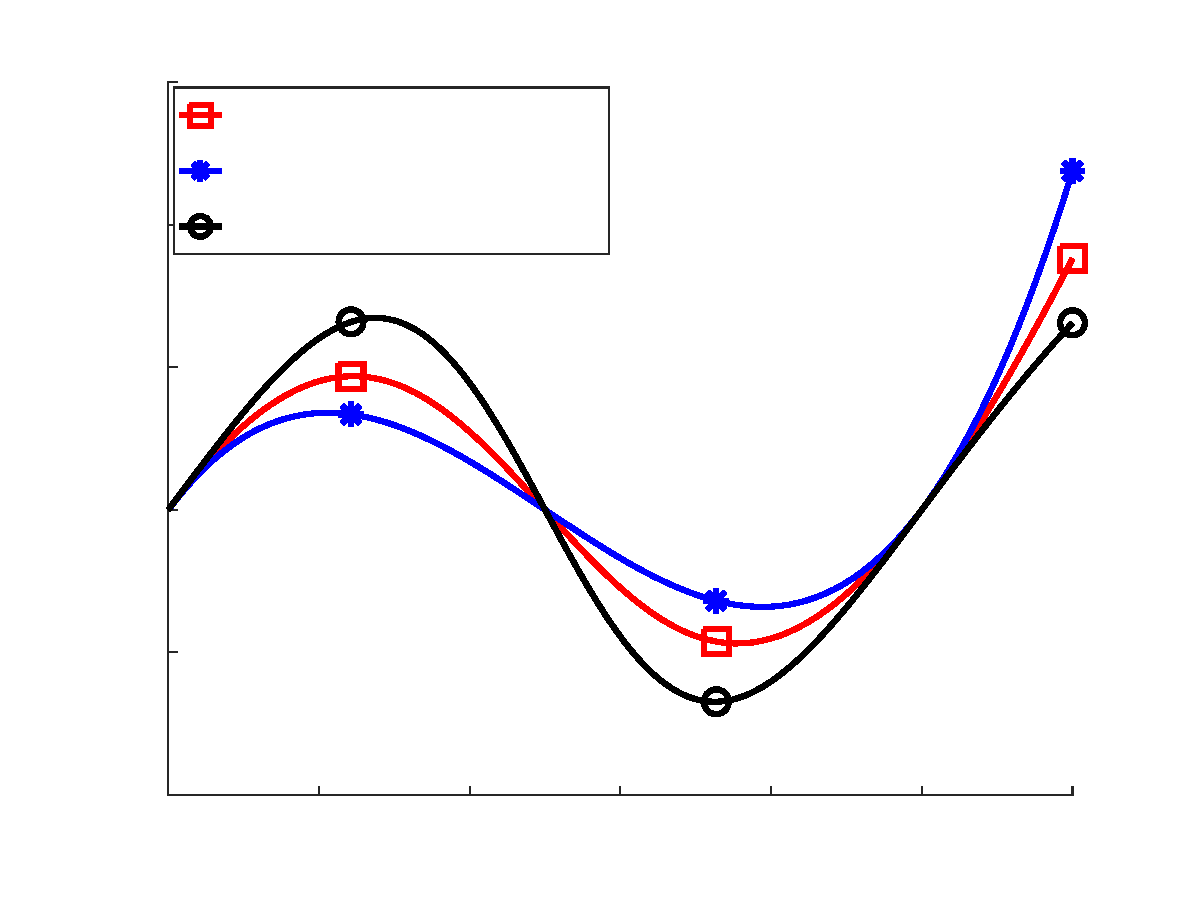
\includegraphics{nonlindef-inc}
\end{picture}%
\begin{picture}(560,420)(0,0)
\fontsize{15}{0}
\selectfont\put(72.8,41.1956){\makebox(0,0)[t]{\textcolor[rgb]{0.15,0.15,0.15}{{0}}}}
\fontsize{15}{0}
\selectfont\put(145.133,41.1956){\makebox(0,0)[t]{\textcolor[rgb]{0.15,0.15,0.15}{{1000}}}}
\fontsize{15}{0}
\selectfont\put(217.467,41.1956){\makebox(0,0)[t]{\textcolor[rgb]{0.15,0.15,0.15}{{2000}}}}
\fontsize{15}{0}
\selectfont\put(289.8,41.1956){\makebox(0,0)[t]{\textcolor[rgb]{0.15,0.15,0.15}{{3000}}}}
\fontsize{15}{0}
\selectfont\put(362.133,41.1956){\makebox(0,0)[t]{\textcolor[rgb]{0.15,0.15,0.15}{{4000}}}}
\fontsize{15}{0}
\selectfont\put(434.467,41.1956){\makebox(0,0)[t]{\textcolor[rgb]{0.15,0.15,0.15}{{5000}}}}
\fontsize{15}{0}
\selectfont\put(506.8,41.1956){\makebox(0,0)[t]{\textcolor[rgb]{0.15,0.15,0.15}{{6000}}}}
\fontsize{15}{0}
\selectfont\put(67.8,46.2){\makebox(0,0)[r]{\textcolor[rgb]{0.15,0.15,0.15}{{-10}}}}
\fontsize{15}{0}
\selectfont\put(67.8,114.66){\makebox(0,0)[r]{\textcolor[rgb]{0.15,0.15,0.15}{{-5}}}}
\fontsize{15}{0}
\selectfont\put(67.8,183.12){\makebox(0,0)[r]{\textcolor[rgb]{0.15,0.15,0.15}{{0}}}}
\fontsize{15}{0}
\selectfont\put(67.8,251.58){\makebox(0,0)[r]{\textcolor[rgb]{0.15,0.15,0.15}{{5}}}}
\fontsize{15}{0}
\selectfont\put(67.8,320.04){\makebox(0,0)[r]{\textcolor[rgb]{0.15,0.15,0.15}{{10}}}}
\fontsize{15}{0}
\selectfont\put(67.8,388.5){\makebox(0,0)[r]{\textcolor[rgb]{0.15,0.15,0.15}{{15}}}}
\fontsize{14}{0}
\selectfont\put(289.8,23.1956){\makebox(0,0)[t]{\textcolor[rgb]{0.15,0.15,0.15}{{Desplazamiento: (-$w$)}}}}
\fontsize{14}{0}
\selectfont\put(38.8,217.35){\rotatebox{90}{\makebox(0,0)[b]{\textcolor[rgb]{0.15,0.15,0.15}{{Carga: (-$P$ $\times \, 10^{+6}$)}}}}}
\fontsize{13}{0}
\selectfont\put(100.802,372.5){\makebox(0,0)[l]{\textcolor[rgb]{0,0,0}{{$P_E$: Def. Unit. Ing. Rotada}}}}
\fontsize{13}{0}
\selectfont\put(100.802,345.833){\makebox(0,0)[l]{\textcolor[rgb]{0,0,0}{{$P_G$: Def. Unit. de Green}}}}
\fontsize{13}{0}
\selectfont\put(100.802,319.166){\makebox(0,0)[l]{\textcolor[rgb]{0,0,0}{{$P_L$: Def. Unit. Log. Rotada}}}}
\end{picture}
}
	\caption{Curvas carga-desplazamiento para distintas medidas de deformación.}
	\label{fig:nonlindef}
\end{figure}


Se puede ver cómo en las posiciones con pequeñas deformaciones los resultados de las distintas medidas de deformación coinciden (es decir para $w \approx 0$ y $w\approx5000$), mientras que en las posiciones con mayores deformaciones unitarias, los resultados dados por las distintas medidas de deformación difieren. %
%
La tensión de Green se corresponde con el comportamiento más flexible.

Cabe indicar que en el cálculo de $\sigma_L$ se asumió que el volumen de la barra era constante.

Adicionalmente, se utilizó la misma relación constitutiva con un módulo $E$ fijo para todas las deformaciones unitarias vistas. Es claro que imponer la misma relación lineal a distintas medidas de tensión y deformación resulta en distintas predicciones en la hipótesis de grandes deformaciones unitarias. Un tratamiento más detallado de estos temas corresponde al análisis con grandes deformaciones unitarias, lo cual está fuera del alcance de este curso.

Como conclusión a los conceptos presentados en este capítulo, se vieron distintas medidas de deformación unitarias no lineales respecto de los desplazamientos. Cada una se relaciona a través del PTV a una medida de tensión conjugada. Se vieron las equivalencias tanto entre medidas de deformación como entre medidas de tensión y se introdujo la medida de tensión ``real'' de Cauchy. La equivalencia tanto entre medidas de tensiones y medidas de deformaciones fue mostrada para el caso de pequeñas deformaciones unitarias.

%En secciones siguientes, se utilizará la deformación de Green como la base de desarrollo de elementos finitos de barra para grandes desplazamientos y rotaciones, manteniendo pequeñas deformaciones unitarias.

El código de Octave usado para generar la Figura~\ref{fig:nonlindef} se presenta en el Código~\ref{cod:nonlinstrain}.

\lstinputlisting[caption = {Medidas de deformación no lineales - Gráfico comparativo.}\label{cod:nonlinstrain}]{../src/MedidasDefNoLineal.m}















\section{Método de Elementos Finitos Incremental}\label{FEM}

% justificacion de usar sol num
Para realizar el análisis no lineal de estructuras es necesario contar con métodos matemáticos que permitan resolver las ecuaciones del principio de trabajos virtuales y obtener las configuraciones de equilibrio para cada carga considerada. %
%
% recordar que ptv, ahora q las medidas de def son no lineales, es un sistema de ecs no lineales
Dado que la deformación es una función no lineal de los desplazamientos, las ecuaciones del principio de trabajos virtuales consisten en un sistema de ecuaciones no lineales. %
%
% soluciones numericas en aplicacion practica
Las soluciones analíticas de estas ecuaciones permiten comprender conceptos estructurales importantes de cada estructura, sin embargo estas son obtenibles únicamente para esquemas estructurales de tamaño reducido. %
%
En esta sección se hará foco en métodos utilizados para la obtención de soluciones numéricas de las ecuaciones del PTV. %
% -----------------------------------------


En esta sección se describe un método numérico basado en el Método de Newton-Raphson y el Método de los Elementos Finitos para la resolución del principio de trabajos virtuales. %
%
El desarrollo es presentado utilizando una notación y metodología similares a las utilizadas en la literatura de referencia \citep{crisfield1996non,DeSouzaNeto2008,DeBorst2012}, en la cual la formulación es usualmente llamada \textit{Total Lagrangian Formulation}. %
% -----------------------------------------------------------


\subsection{Método de los Elementos Finitos en análisis lineal de reticulados}

%
La necesidad de resolver problemas de análisis de estructuras de grandes dimensiones de forma eficiente llevó al desarrollo del Método de los Elementos Finitos (MEF) en la segunda mitad del siglo XX. %
%
\citeauthor{Zienkiewicz1972} es considerado como uno de los líderes más importantes en el proceso de concepción del método orientado al análisis de estructuras \citep{Zienkiewicz1972}, seguido por \citeauthor{Bathe1982} y \citeauthor{Hughes1987a} quienes también lideraron el desarrollo del método para la resolución de diversos problemas de ingeniería mecánica \citep{Bathe1982,Hughes1987a}. %
%
En las décadas posteriores, y gracias al creciente acceso a computadoras, el método se convirtió en la herramienta de referencia para la resolución práctica de problemas en diversas disciplinas de la ingeniería, particularmente en ingeniería estructural \citep{Onate2013,Zienkiewicz2014}. %
%
En esta sección se presentan, de forma esquemática, los conceptos básicos del MEF para el análisis lineal de estructuras de barras articuladas.
% ----------------------------------------------------------------



Sea una estructura que ocupa una cierta región del espacio, se establece una subdivisión de dicha región en \textit{elementos}, los cuales forman una \textit{malla}. %
%
En el caso de estructuras reticuladas cada barra representa un elemento. %
%
Considerando en este caso que se tiene una estructura reticulada plana formada por $n_e$ barras, el desplazamiento en el plano de todo punto de cada barra puede ser interpolado a partir del desplazamiento de sus nodos, esto es:
%
\begin{equation}
u(x^e) = \bfN_{loc}^e(x^e) \bfu_{loc}^e,
\qquad
\bfN_{loc}^e = \left[ \begin{matrix}
\frac{\ell_0^e - x^e}{\ell_0^e} & 0 & \frac{x^e}{\ell_0^e} & 0
\end{matrix} \right],
\end{equation}
%
donde $\bfu^e$ es el vector de desplazamientos nodales del elemento (o barra) $e$, $\ell_0^e$ es el largo del elemento y $x^e\in[0,\ell_0^e]$ es una coordenada auxiliar local del elemento en la configuración de referencia. %
%
A pesar de que otras interpolaciones pueden ser consideradas, son utilizadas funciones lineales, las cuales son adecuadas para problemas de barras con fuerza de volumen aplicadas despreciables.
% -------------------------


Aplicando la relación lineal entre desplazamientos y deformación (ingenieril) se obtiene la expresión:
%
\begin{equation}\label{eqn:expeps}
\varepsilon^e =  \bfb_{L,loc}^e(x^e) \bfu_{loc}^e
\quad
\text{con}
\quad
\bfb_{L,loc}^e = \frac{1}{\ell_0^e} \left[ \begin{matrix}
-1 & 0 & 1 & 0
\end{matrix} \right].
\end{equation}
% ------------------------------

Para poder aplicar el PTV a toda la estructura es necesario considerar un sistema de coordenadas global, para esto se realiza un cambio de base:
%
\begin{equation}
\bfu^e = \bfQ^e \bfu^e_{loc} \quad \text{con} \quad \bfQ^e = \left[
\begin{matrix}
\cos(\phi^e) & -\sin(\phi^e) & 0 & 0 \\
\sin(\phi^e)  & \cos(\phi^e) & 0 & 0 \\
0  & 0 & \cos(\phi^e) &-\sin(\phi^e) \\
0  & 0 & \sin(\phi^e) & \cos(\phi^e) \\
\end{matrix}\right],
\end{equation}
%
donde se puede ver que $\phi^e$ es el ángulo medido en sentido antihorario desde el eje $x$ del sistema global al eje $x$ local y $\bfQ^e$ es la matriz de cambio de base del sistema local al global o la matriz asociada a la transformación lineal $_{global}(\bfI)_{loc}$.
% -------------------------------------------


Sustituyendo en la Ecuación~\eqref{eqn:expeps} se obtiene la expresión:
%
\begin{equation}\label{eqn:exprepslin}
\varepsilon^e =  \bfb_L^e \bfu^e,
\qquad
\bfb_L^e = \frac{1}{\ell_0^e} \left[ \begin{matrix}
-\cos(\phi^e) & -\sin(\phi^e) & \cos(\phi^e) & \sin(\phi^e)
\end{matrix} \right],
\end{equation}
%
y sustituyendo en la ecuación constitutiva se obtiene la tensión en función de los desplazamientos nodales:
%
\begin{equation}
\sigma^e = E \bfb_L^e \bfu^e,
\end{equation}
donde $E$ es el módulo de elasticidad de la barra. %
%

Se está en condiciones ahora de sustituir las expresiones en el principio de trabajos virtuales, comenzando por el trabajo interno. El trabajo interno de una barra está dado por:
%
\begin{equation}
\delta W_{\text{int}}(\bfu^e) %
= \int_{\ell_0^e}  \delta \varepsilon^e \, \sigma^e \, A \, \dif x %
%
= \int_{\ell_0^e} \left( \delta \bfu^e\right)^{\text{T}} \left( \bfb_L^e\right)^{\text{T}} E A \bfb_L^e \bfu^e \, \dif x  %
%
= \left( \delta \bfu^e \right)^{\text{T}} \bff^e_{\text{int}}(\bfu^e),
\end{equation}
%
donde fue definido el vector de fuerzas internas del elemento $\bff^e_{\text{int}}(\bfu^e)$. %
%
Este vector de fuerzas internas puede ser escrito de forma compacta como:
%
\begin{equation}
\bff^e_{\text{int}} (\bfu^e) = \bfK_L^e \bfu^e,
\end{equation}
%
donde la matriz $\bfK^e_L$ es llamada matriz de rigidez del elemento $e$ y está dada por:
%
\begin{equation}
\bfK_L^e = \int_{\ell^e} \left( \bfb_L^e\right)^{\text{T}} E A \bfb_L^e \, \dif x.
\end{equation}
%

El trabajo virtual interno del conjunto de la estructura puede ser escrito como la suma del trabajo de todas las barras:
%
\begin{equation}
\delta W_{\text{int}}(\bfu) = \sum_{e=1}^{n_e} \left(\delta \bfu^e\right)^{\text{T}} \bfK_L^e \bfu^e = \left(\delta \bfu \right)^{\text{T}} \bfK_L \bfu,
\end{equation}
%
donde para la matriz $\bfK_L$ y el vector $\bfu$ incluyen todos los grados de libertad de la estructura. %
%
Para obtenerlos se aplica el procedimiento llamado \textit{ensamblado}, el cual consiste en considerar de forma acoplada todos los grados de libertad de la estructura y es denotado como:
%
\begin{equation}
\bfK_L = \assem_{e=1}^{n_e} \bfK_L^e \qquad   \bfu = \assem_{e=1}^{n_e} \bfu^e.
\end{equation}
%
Se puede también expresar el vector global de fuerzas internas de la estructura como $\bff_{\text{int}} (\bfu) = \bfK_L \bfu$. %
%
El ensamblado es presentado en forma más completa en la Sección~\ref{sec:ensamblado}. 

Sea una estructura de barras formada por 8 nodos, sea una barra definida por los nodos 3 y 7 tal que $x^e=0$ corresponde al nodo 3. %
%
Los grados de libertad de esos nodos en el vector de desplazamientos globales serán: $[ 2\times 3 -1$, $2\times 3, 2\times 7 -1$, $2\times 7]$. %
%
En una implementación del MEF es de utilidad contar con una función que permita calcular los grados de libertad vinculados a un conjunto arbitrario de nodos. %
%
En la herramienta ONSAS se utiliza una función para dicho fin, llamada \textit{nodes2dofs}, cuyo código se sugiere mirar.


El principio de trabajos virtuales establece entonces la igualdad entre el trabajo virtual interno y el trabajo virtual externo:
\begin{equation}
\delta \bfu^{\text{T}} \bff_{\text{int}} =
\delta \bfu^{\text{T}} \bff_{\text{ext}}  \qquad \forall \delta \bfu \in \mcV,
\end{equation}
lo cual, sustituyendo las expresiones anteriores, es equivalente a la resolución del sistema lineal de ecuaciones:
%
\begin{equation}
\boxed{
	\bfK_L \bfu = \bff_{\text{ext}}.
}
\end{equation}
La resolución del sistema es realizada tomando en cuenta las condiciones de contorno de desplazamiento conocido en los grados de libertad correspondientes. %
%
En el caso de desplazamientos impuestos no nulos se agrega un término correspondiente al término independiente. Por simplicidad no se considera dicho caso en este material. %
% -------------------------------------


\subsection{Método de Newton-Raphson aplicado al PTV}

En esta sección se aplica el método de Newton-Raphson a la resolución de las ecuaciones del PTV para estructuras de barras considerando la medida de deformación de Green y un único estado de cargas externas aplicado a la estructura.

\subsubsection{Elemento finito de barra de Green}

Tal como se vió en la Sección~\ref{Sec:PTVBielas}, al analizar bielas la única componente del tensor de tensiones que realiza trabajo es la axial. %
%
Considerando la Ecuación~\eqref{PTVBielaSStrain} y asumiendo que la sección transversal del elemento es uniforme con área $A_0$ se obtiene la siguiente expresión del PTV para bielas:
%
\begin{equation}\label{eqn:ptvbielaA0}
A_0 \int_{\ell_0} \sigma(x_0) \delta \varepsilon \, \dif x_0 = \delta \bfu^{\text{T}} \bff_{\text{ext}}   \qquad \forall \delta \bfu \in \mcV
\end{equation}
%
donde $\sigma(x_0)$ representa la tensión de Green en cada punto con coordenadas locales de referencia $x_0$ y $\bff_{\text{ext}}$ las fuerzas externas nodales. %
%
En el caso de un único elemento las fuerzas externas estarían dadas por:
%
\begin{equation}
\bff_{\text{ext}} = \left[ f_{\text{ext},1,x}, f_{\text{ext},1,y}, f_{\text{ext},2,x}, f_{\text{ext},2,y} \right]^{\text{T}}.
\end{equation}

Respecto a las tensiones, para elementos de biela, sometidos a fuerzas en los nodos, la deformación axial y la tensión es uniforme, por lo que se puede omitir la dependencia de $x_0$.

En la \autoref{fig:truss1f} se muestra un elemento de barra en la configuración de referencia y en la configuración deformada de equilibrio correspondiente. %
%
\begin{figure}[htb]
	\centering
	\def\svgwidth{0.7\textwidth}
    \input{../fig/ptv_truss1f.pdf_tex}
	\caption{Esquema de desplazamientos y fuerzas de elemento de barra.}
	\label{fig:truss1f}
\end{figure}
%
Se muestra también, esquematizada con línea azul a trazos, una configuración virtual que puede adquirir la barra.


Para realizar un procedimiento similar al de elementos finitos lineal, se comienza buscando una expresión para las fuerzas internas del elemento $\bff_{\text{int}}$. %
%
Para esto se deberá obtener una expresión para la variación de la deformación axial debida a los desplazamientos virtuales. %


La expresión del largo de la barra en la configuración de referencia $\ell_0$ está dada por:
%
\begin{equation}
\ell_0 = \sqrt{ \left( \bfx_2 - \bfx_1\right)^{\text{T}} \left( \bfx_2 - \bfx_1\right)},
\end{equation}
%
mientras que el largo en la configuración deformada $\ell$ está dado por:
%
\begin{equation}
\ell (\bfu)
= \sqrt{
	\left( \bfx_2+\bfu_2 - \bfx_1 -\bfu_1 \right)^{\text{T}}
	\left( \bfx_2+\bfu_2 - \bfx_1 -\bfu_1 \right)
}.
\end{equation}
%


Dado que se considera la medida de deformación de Green, se sustituyen estas expresiones en la Ecuación~\eqref{GreenStrain} y se desarrolla, obteniendo:
%
\begin{equation}\label{eqn:eceps}
\varepsilon(\bfu) 
= \frac{1}{2} \frac{\ell(\bfu)^2 - \ell_0^2}{\ell^2_0} 
= \frac{  \left(\bfx_{2}-\bfx_1 \right)^{\text{T}} \left(\bfu_{2}-\bfu_1 \right) }{\ell^2_0}
+ \frac{1}{2} \frac{ \left(\bfu_{2}-\bfu_1 \right)^{\text{T}} \left(\bfu_{2}-\bfu_1 \right) }{\ell^2_0}.
\end{equation}
%
Se confirma que la deformación es cuadrática en los desplazamientos. %
%
Se considera ahora la relación con la notación usual del MEF para el vector de desplazamientos, en su expresión matricial:
%
\begin{equation}\label{eqn:expru21}
\bfu_2 - \bfu_1 = \left[ \begin{matrix}
-1 & 0 &  1 &  0 \\
0 & -1 &  0 &  1 \\
\end{matrix} 
\right] \bfu^e
\qquad
\bfx_2 - \bfx_1 = \left[ \begin{matrix}
-1 & 0 &  1 &  0 \\
0 & -1 &  0 &  1 \\
\end{matrix} 
\right] \bfx^e
\end{equation}
%
donde $\bfu^e$ es el vector de desplazamientos nodales y $\bfx^e$ el vector de posiciones iniciales de los nodos, ambos dados por las expresiones:
%
\begin{equation}
\bfx^e = \left[ x_1, y_1, x_2, y_2 \right]^{\text{T}}
\quad \text{y} \quad
\bfu^e = \left[ u_1, v_1, u_2, v_2 \right]^{\text{T}}.
\end{equation}
%


Sustituyendo las expresiones de la Ecuación~\eqref{eqn:expru21} en la Ecuación~\eqref{eqn:eceps} se obtiene la relación entre deformación de Green y desplazamientos nodales en forma matricial, dada por:
%
\begin{equation}
\varepsilon (\bfu^e) = \frac{1}{\ell_0^2} 
(\bfx^e)^{\text{T}} \bfG^e \bfu^e +  \frac{1}{2} \frac{1}{\ell_0^2}  (\bfu^e)^{\text{T}} \bfG^e \bfu^e
\end{equation}
%
donde
%
\begin{equation}
\bfG^e =
\left[\begin{matrix}
1 & 0 & -1 & 0\\
0 & 1 &0 & -1\\
-1 & 0& 1 & 0\\
0 & -1 &0 & 1\\
\end{matrix}
\right].
\end{equation}


Es importante destacar que la definición de deformación considerada provee un valor uniforme a lo largo de la barra, lo que es coherente con barras con cargas aplicadas en los extremos. %
%


Será de utilidad contar con una expresión matricial compacta de la forma:
%
\begin{equation}
\varepsilon (\bfu^e) = \bfb^e_1 \bfu^e +  \frac{1}{2} \bfb_{2}^e(\bfu^e) \bfu^e
\end{equation}
%
donde
%
\begin{equation}\label{eqn:exprbs}
\bfb^e_1 =  \frac{1}{\ell_0^2} 
(\bfx^e)^{\text{T}} \bfG^e
\quad
\text{y}
\quad
\bfb^e_2 (\bfu^e) = \frac{1}{\ell_0^2}  (\bfu^e)^{\text{T}} \bfG^e.
\end{equation}


%Es importante destacar que $\bfb_1^e$ depende de $\bfx^e$ sin embargo se optó por omitirlo este argumento en la notación ya que $\bfx^e$ no es una variable a determinar.

Se puede ahora calcular la variación de la deformación $\delta\varep$ debida a un desplazamiento virtual $\delta\bfu$, dada por:
%
\begin{equation}
\delta \varep =  \frac{\partial \varep}{\partial \bfu}(\bfu) \delta \bfu.
\end{equation}

Previo a realizar el cálculo se aclara que la notación considerada para gradientes de funciones escalares o vectoriales es dado por vectores fila, decir, dada una función vectorial $\bfg(\bfu) :\bbR^n \rightarrow \bbR^m $, se cumple:
%
\begin{equation}
\bfg(\bfu+\delta\bfu) \approx \bfg(\bfu) + \frac{\partial \bfg }{\partial \bfu}(\bfu) \delta \bfu
\end{equation}
%
siendo $\frac{\partial \bfg }{\partial \bfu}(\bfu)$ una matriz tal que la entrada de la $i$-ésima fila y $j$-ésima columna está dada por $ \left( \frac{\partial \bfg }{\partial \bfu}(\bfu) \right)_{ij} =  \frac{\partial g_i }{\partial u_j }(\bfu)$. %
%
Dado que el vector $\delta \bfu$ es un vector columna, el producto del segundo término del miembro derecho está bien definido.


%rivada de f(x)*g(x) respecto de x es igual a (fx)^T * g(x) + f(x) * Gx(x)


Operando se obtiene:
%
\begin{equation} \label{eqn:derivepsilon}
\frac{\partial \varep}{\partial \bfu }(\bfu)  =  \bfb_1^e + \bfb_2^e(\bfu),
\end{equation}
%
por lo que la variación de la deformación está dada por:
%
\begin{equation}\label{eqn:variacionepsilon}
\delta \varep = \left( \bfb_1^e + \bfb_2^e(\bfu) \right) \delta \bfu.
\end{equation}


\cajaactividad{Demostrar la identidad de la Ecuación~\eqref{eqn:variacionepsilon} de dos formas:
	\begin{itemize}
		\item utilizando la definición y propiedades de la derivada,
		\item realizando una aproximación de primer orden de la diferencia $\varepsilon (\bfu^e + \delta \bfu^e) - \varepsilon (\bfu^e)$. %
	\end{itemize}
}

%
%Sustituyendo y desarrollando se tiene:
%%
%\begin{equation}
%  \delta \varep = 
%   \bfb_1^e \delta \bfu^e + \frac{1}{\ell_0^2} (\delta \bfu^e)^{\text{T}} \bfG^e \bfu^e   
%   + \frac{1}{2} \frac{1}{\ell_0^2} (\delta \bfu^e)^{\text{T}} \bfG^e \delta\bfu^e.
%\end{equation}

%Transponiendo el primer término (que es un escalar) y despreciando el tercer término por considerar pequeños desplazamientos virtuales se obtiene:
%%
%\begin{equation}
%\delta \varep = 
%(\delta  \bfu^e)^{\text{T}} (\bfb_1^e)^{\text{T}} + \frac{1}{\ell_0^2} (\delta \bfu^e)^{\text{T}} \bfG^e \bfu^e
%= (\delta  \bfu^e)^{\text{T}} (\bfb_1^e + \bfb_2^e(\bfu^e) )^{\text{T}} .
%\end{equation}

Dado que $\delta \varep$ es un escalar, es igual a su traspuesta, por lo que se traspone la Ecuación~\eqref{eqn:variacionepsilon} y se sustituye en el miembro izquierdo de la Ecuación~\eqref{eqn:ptvbielaA0} obteniendo %
%
\begin{equation}
(\delta  \bfu^e)^{\text{T}} \left( A_0 \int_{\ell_0}  (\bfb_1^e)^{\text{T}} \sigma^e \dif x + A_0 \int_{\ell_0}  \bfb_{2}^e(\bfu^e)^{\text{T}} \sigma^e  \, \dif x \right) =
(\delta  \bfu^e)^{\text{T}} \bff_{\text{int}}^e(\bfu^e).
\end{equation}

El miembro del trabajo virtual interno puede ser escrito en función del vector de fuerzas internas definido como:
%
\begin{equation}
\delta  W_{\text{int}}(\bfu^e) = (\delta  \bfu^e)^{\text{T}} \bff_{\text{int}}^e(\bfu^e),
\end{equation}
%
donde el vector de fuerzas internas está dado por:
%
\begin{equation}
\bff_{\text{int}}^e(\bfu^e) = A_0 \int_{\ell_0}  (\bfb_1^e)^{\text{T}} \sigma^e \dif x + A_0 \int_{\ell_0}  \bfb_{2}^e(\bfu^e)^{\text{T}} \sigma^e  \, \dif x .
\end{equation}

Usando que la deformación es uniforme en la barra y que la tensión depende únicamente de la deformación, se obtiene la siguiente expresión 
%
\begin{equation}
\bff_{\text{int}}^e(\bfu^e) %
%
= A_0 \sigma^e  \ell_0  (\bfb_1^e +  \bfb_{2}^e(\bfu^e) )^{\text{T}}.
\end{equation}


%Definiendo
%\begin{equation}
% \bfb(\bfu^e)= \bfb_1^e + \bfb^e_2(\bfu^e), \quad \text{con} \quad  \bfb^e_{2}(\bfu^e) = \frac{1}{\ell_0^2} \bfG^e \bfu^e
%\end{equation}
%
%se tiene
%\begin{equation}
%\bff_{\text{int}}^e(\bfu^e) = A_0 \int_{\ell_0}  (\bfb^e(\bfu^e))^{\text{T}} \sigma \dif x.
%\end{equation}

\subsubsection{Ensamblado} \label{sec:ensamblado}

% ------------------------------------------------------------------------------
Para introducir el proceso de ensamblado se considera un ejemplo simple: una estructura formada por 2 barras articuladas. %
%
La barra 1 une los nodos 1 y 2, mientras que la barra 2 une los nodos 3 y 2 (en ambos casos se consideró una orientación definiendo ejes locales). %
%
Ambas barras tienen sección transversal de área $A_0$ y largo $\ell_0$. %
% ------------------------------------------------------------------------------


% ------------------------------------------------------------------------------
Sea un vector columna de desplazamientos virtuales de la estructura, formado por los vectores columna de desplazamientos de los tres nodos: $\delta \bfu^{\text{T}} = \left[ \delta\bfu_1^{\text{T}}, \delta\bfu_2^{\text{T}},  \delta\bfu_3^{\text{T}} \right]$. %
%
El trabajo virtual de las fuerzas internas está dado por la suma de los trabajos virtuales de cada barra:
%
\begin{equation}
\delta  W_{ \text{int} } (\bfu) %
%
=
\left[ \delta\bfu_1^{\text{T}},  \delta\bfu_2^{\text{T}} \right] 
\left[ 
\begin{matrix}
\bff_{\text{int},1}^1  \\
\bff_{\text{int},2}^1 
\end{matrix}
\right] 
+
\left[ \delta\bfu_3^{\text{T}},  \delta\bfu_2^{\text{T}} \right] 
\left[ 
\begin{matrix}
\bff_{\text{int},1}^2  \\
\bff_{\text{int},2}^2 
\end{matrix}
\right] 
%\nonumber\\
%\dots &+&
%\left[ \delta\bfu_3^{\text{T}},  \delta\bfu_2^{\text{T}} \right] \sigma^2 A_0 \ell_0  \frac{1}{\ell_0^2}  \bfG^e 
%\left[ 
%\begin{matrix}
%\bfx_3^e + \bfu_3^e \\
%\bfx_2^e + \bfu_2^e
%\end{matrix}
%\right] \nonumber
\end{equation}
donde $\bff_{\text{int},i}^e$ representa el vector columna de fuerzas internas correspondiente al nodo $i$ del elemento $e$. %
%
Desarrollando y factorizando se tiene
%
\begin{equation}
\delta  W_{ \text{int} } (\bfu) %
%
=
\left[ \delta\bfu_1^{\text{T}},  \delta\bfu_2^{\text{T}}, \delta\bfu_3^{\text{T}} \right] 
\left[ 
\begin{matrix}
\bff_{\text{int},1}^1  \\
\bff_{\text{int},2}^1 + \bff_{\text{int},2}^2 
\\
\bff_{\text{int},1}^2 
\end{matrix}
\right].
\end{equation}

Esta factorización permite escribir el trabajo interno en función de un único vector de fuerzas internas
%
\begin{equation}
\delta  W_{ \text{int} } (\bfu) %
%
=
\delta\bfu
\,
\bff_{\text{int}},
\end{equation}
%
donde el vector $\bff_{\text{int}}$ es el resultado del ensamblado, denotado como:
%
\begin{equation}
\bff_{\text{int}}(\bfu) = \assem_{e=1}^{n_e} \bff^e_{\text{int}}(\bfu^e) 
%=\assem_{e=1}^{n_e} A_0 \left( \int_{\ell_0}  (\bfb^e (\bfu^e) )^{\text{T}} \sigma(\bfu^e) \dif x \right)
=\assem_{e=1}^{n_e} A^e_0   (\bfb^e (\bfu^e) )^{\text{T}} \sigma(\bfu^e) \ell^e_0.
\end{equation}
%
siendo $\ell_0^e$ y $A_0^e$ los largos y áreas de las secciones transversales del elemento $e$-ésimo. %
%
En esta última ecuación se hizo explícita la dependencia de $\sigma$ respecto a los desplazamientos y también se introdujo la notación abreviada
%
\begin{equation}
\bfb^e (\bfu^e) = \bfb_1^e + \bfb_2^e (\bfu^e).
\end{equation}

El principio de trabajos virtuales de la estructura completa está dado entonces por la expresión:
%
\begin{equation}
\delta \bfu^{\text{T}} \left( \bff_{\text{int}}(\bfu) - \bff_{\text{ext}} \right) = 0 \qquad \forall \delta \bfu \in \mcV
\end{equation}
%
por lo tanto, utilizando que esta igualdad se debe cumplir para cualquier $\delta \bfu$, se llega a que encontrar la solución del PTV es equivalente a resolver el siguiente sistema de ecuaciones no lineales:
%
\begin{equation}\label{eqn:residuo}
\boxed{
	\bfr(\bfu) = \bff_{\text{int}}(\bfu) - \bff_{\text{ext}} = \bszer,
}
\end{equation}
%
donde $\bfr$ representa el vector de fuerzas nodales residuales o fuerzas \textit{no equilibradas}.

% ---------------------



\subsubsection{Iteración de Newton-Raphson} \label{sec:iterNR}

Se está ahora en condiciones de aplicar un método iterativo para sistemas de ecuaciones no lineales como el de Newton-Raphson presentado en la Sección~\ref{sec:NRcap1}. %
%
Este método establece una regla para variar el vector de desplazamientos $\bfu$ hasta obtener una solución de acuerdo al criterio de parada definido. %
%
La expresión de la variación en $\bfu$ está dada por:
%
\begin{equation} \label{eqn:increu}
\bfu^{(k+1)} = \bfu^{(k)} + \Delta \bfu^{(k)},
\end{equation}
%
y la ecuación linealizada que impone el método en cada iteración es
%
\begin{equation}
\bfr \left( \bfu^{(k)} + \Delta \bfu^{(k)} \right) \simeq \bfr(\bfu^{(k)} ) + \frac{\partial \bfr}{\partial \bfu}(\bfu^{(k)})\cdot \Delta \bfu^{(k)} = \bszer,
\end{equation}
%
es decir:
\begin{equation}
\frac{\partial \bfr}{\partial \bfu}(\bfu^{(k)})\cdot \Delta \bfu^{(k)} = -\bfr(\bfu^{(k)} ).
\end{equation}
%
Sustituyendo la expresión de $\bfr$ de la Ecuación~\eqref{eqn:residuo} se obtiene
%
\begin{equation}\label{eqn:sistderivf}
\frac{\partial \bff_{\text{int}}}{\partial \bfu} \left(\bfu^{(k)} \right)   \Delta \bfu^{(k)}
= - \left( \bff_{\text{int}}(\bfu^{(k)} ) - \bff_{\text{ext}} \right).
\end{equation}
%

Se cuenta entonces con las ecuaciones \eqref{eqn:increu} y \eqref{eqn:sistderivf}, que junto con la condición de desplazamiento nulo para carga nula definen el procedimiento numérico a aplicar, similar al descrito en la Ecuación~\eqref{NR2}.


Se deben calcular las derivadas del vector de fuerzas internas, lo cual puede ser realizado para cada elemento dado que el ensamblado es un proceso de suma de términos. %
%
Para calcular la derivada se utiliza la siguiente identidad para derivada de producto de funciones:
$$
\dfrac{\partial g(\bfx)\bff(\bfx)}{\partial \bfx} = \bff(\bfx)\dfrac{\partial g(\bfx)}{\partial \bfx}+g(\bfx)\dfrac{\partial \bff(\bfx)}{\partial \bfx},
$$
con  $g:\mathbb{R}^n\rightarrow \mathbb{R}$ una función escalar y $\bff:\mathbb{R}^n\rightarrow \mathbb{R}^n$ una función vectorial. %

El vector de fuerzas internas es un producto de la función $\sigma$ y el vector columna $\bfb^T$, por lo que se obtiene:
%
\begin{equation}\label{eqn:fueinterna}
\frac{\partial \bff^e_{\text{int}} } {\partial \bfu^e} (\bfu^{(k)}) 
= A_0^e \ell_0^e  \frac{\partial \left(\bfb^e\right)^{\text{T}} }{\partial \bfu^e} (\bfu^{(k)}) \sigma^e(\bfu^{(k)}) 
+ A_0^e \ell_0^e  (\bfb^e(\bfu^{(k)}))^{\text{T}} \frac{ \partial \sigma^e}{\partial \bfu^e}(\bfu^{(k)}).
\end{equation}
%
donde por simplicidad de notación se omitió el superíndice $e$ en el vector $\bfu^k$.

Para el cálculo de la derivada de la tensión se utiliza la regla de la cadena, obteniendo:
%
\begin{equation}
\frac{ \partial \sigma}{\partial \bfu}(\bfu^{(k)}) = \frac{\partial \sigma}{\partial \varep}(\varep(\bfu^{(k)}))\, \frac{\partial \varep}{\partial \bfu}(\bfu^{(k)}).
\end{equation}
%
Usando que el material tiene comportamiento constitutivo lineal, es decir $\sigma = E \varep$, y sustituyendo la expresión de la derivada de $\varep$ dada por la Ecuación~\eqref{eqn:derivepsilon} se obtiene la identidad:
\begin{equation}
\frac{ \partial \sigma^e}{\partial \bfu}(\bfu^{(k)}) = E^e \bfb^e(\bfu^{(k)}).
\end{equation}

Sustituyendo en la Ecuación~\eqref{eqn:fueinterna} y calculando la derivada de $\bfb$ a partir de la Ecuación~\eqref{eqn:exprbs} se obtiene:
%
\begin{equation}
\frac{\partial \bff_{\text{int}}^e } {\partial \bfu^e} (\bfu^{(k)})
= \frac{\sigma^{(k)} A_0 }{\ell_0} \bfG^e
+  (\bfb^e(\bfu^{(k)}))^{\text{T}} \, E^e A_0^e \ell_0^e \, \bfb^e(\bfu^{(k)}).
\end{equation}
%
Resulta conveniente utilizar una expresión matricial de la forma:
%
\begin{equation}
\frac{\partial \bff_{\text{int}} } {\partial \bfu} (\bfu^{(k)}) \Delta \bfu^{(k)} = \bfK_{T}(\bfu^{(k)}) \, \Delta \bfu^{(k)},
\end{equation}
%
donde la matriz $\bfK_T$ es llamada matriz tangente, la cual está dada por:
%
\begin{eqnarray}
\bfK_T(\bfu^{(k)}) &=& \underbrace{E A_0 \ell_0 \bfb^{\text{T}}_{1} \bfb_{1}}_{\bfK_{T1}} \nonumber\\
\dots & +& \underbrace{E A_0 \ell_0 \left( \bfb^{\text{T}}_{1} \bfb_{2}(\bfu^{(k)})  + \bfb^{\text{T}}_{2}(\bfu^{(k)}) \bfb_{1} + \bfb^{\text{T}}_{2}(\bfu^{(k)}) \bfb_{2}(\bfu^{(k)}) \right) }_{\bfK_{T2}(\bfu^{(k)})} \nonumber\\
\dots  & +& \underbrace{\frac{\sigma^{(k)} A_0}{\ell_0} \bfG}_{\bfK_\sigma},
\end{eqnarray}
%
donde nuevamente se omitió el superíndice $e$ por simplicidad de la notación. %
%
La matriz $\bfK_{T1}$ es la matriz de rigidez lineal, la matriz $\bfK_{T2}$ es llamada matriz de desplazamiento inicial y la matriz $\bfK_{\sigma}$ la matriz de tensión inicial o matriz geométrica, donde $\bfG$ es la matriz obtenida luego del proceso de ensamblado de $\bfG^e$.


La matriz $\bfK_{T1}$ es la única que es considerada al realizar análisis lineales, es por esto que también pueden agruparse como una matriz de rigidez de análisis lineal y otra del análisis no lineal:
\begin{equation}
\bfK_L = \bfK_{T1} \qquad \bfK_{NL} (\bfu^{(k)}) = \bfK_{T2}(\bfu^{(k)}) + \bfK_{\sigma}(\bfu^{(k)})
\end{equation}
%
donde se debe destacar que la dependencia de $\bfK_{\sigma}$ respecto a $\bfu^k$ está dada a través de las tensiones en la iteración actual $\sigma^{(k)}$.

Sustituyendo en la Ecuación~\eqref{eqn:sistderivf} y realizando también el ensamblado se obtiene el sistema a resolver en cada iteración del método NR:
%
\begin{equation}
\boxed{
	\bfK_{T} (\bfu^{(k)}) \, \Delta \bfu^{(k)} = \bff_{\text{ext}} - \bff_{\text{int}}(\bfu^{(k)})
}
\end{equation}

En la herramienta ONSAS los procesos de ensamblado de la matriz tangente y del vector de fuerzas internas son realizados en la función \textit{assembler}.

\subsubsection{Criterios de parada}
En cada iteración el sistema es resuelto, los valores $\bfu$ son actualizados, $\sigma^k$ y $\bff_{\text{int}}$ son calculados y se evalúa si se verifican las condiciones de parada. %
%
Algunos de los criterios de parada que se pueden considerar son:
%
\begin{enumerate}
	\item Convergencia en desplazamientos:
	$$ \dfrac{ \|\Delta \bfu^{(k)} \|}{\| \bfu^{(k)} \|} < tol_u $$
	\item Fuerzas residuales despreciables:
	$$ \dfrac{\|\bfr ( \bfu^{(k+1)} ) \|}{\| \bff_{\text{ext}} \|} < tol_f $$
	\item Máximo de iteraciones: al igual que en cualquier otro método iterativo es necesario definir un criterio de parada vinculado a una cantidad máxima de iteraciones $max_{it}$.
	$$k > max_{it}$$
\end{enumerate}


En el Algoritmo~\ref{alg:mefnl1carga} se muestra un pseudocódigo del método considerando como criterio de parada la variación en desplazamientos. %
%
Se puede optar por incluir el criterio de parada basado en des-balance de fuerzas también.

\begin{algorithm}
	\caption{Método de Elementos Finitos no lineales para un estado de cargas.}
	\label{alg:mefnl1carga}
	\begin{algorithmic}[1]
		\STATE Asignar punto inicial: $\bfu^{(k)} \leftarrow \bfu^0$ y $\Delta \bfu^{(k)} = \bszer$.
		\STATE Calcular: $\sigma^{(k)} \leftarrow \sigma(\bfu^{(k)})$.
		\WHILE{$\|\Delta \bfu^{(k)} \|> tol_u \|\bfu^{(k)} \|$ \& $k< max_{it}$}
		\STATE Calcular: $\bfK_T \leftarrow \bfK_T(\bfu^{(k)} )$
		\STATE Calcular: $\bff_{\text{int}}^{(k)} \leftarrow \bff_{\text{int}}(\bfu^{(k)} )$.
		\STATE Resolver: $\bfK_T \Delta \bfu^{(k)} = \bff_{\text{ext}} - \bff_{\text{int}}^{(k)}$
		\STATE Actualizar: $k \leftarrow k + 1$, $\bfu^{(k)} \leftarrow \bfu^{(k)} + \Delta \bfu^{(k)}$ y $\sigma^{(k)} \leftarrow \sigma(\bfu^{(k)})$.
		\ENDWHILE
	\end{algorithmic}
\end{algorithm}



\subsubsection{Implementación en Octave y ejemplo}\label{sec:implem}

% --------------------------------------------------------------------
En esta sección se presenta una implementación del método presentado para calcular los desplazamientos de estructuras reticuladas planas. %
%
Como ejemplo se considera la misma estructura de la Sección~\ref{sec:cerchamises} la cual, a pesar de su simpleza, permite observar y analizar comportamientos presentes en estructuras más complejas. %
%
Se considera la estructura simétrica formada por dos barras para resolver un problema que requiere el ensamblado de matrices. %
% ------------------------------------------------------------


En el Código~\ref{cod:cerchamises} se presenta la implementación en GNU-Octave del algoritmo, en la cual se utilizaron notaciones y comentarios con la intención de facilitar la vinculación de las sentencias y variables definidas con el desarrollo presentado en esta sección. %

\lstinputlisting[caption = {Método de Newton-Raphson aplicado a reticulado de Von Mises.}\label{cod:cerchamises}]{../src/cerchamises.m}

En la Figura~\ref{fig:defmises} se muestran los resultados obtenidos al ejecutar el Código presentado. %



\begin{figure}[htb]
	\centering
	\resizebox{.49\linewidth}{!}{% Title: gl2ps_renderer figure
% Creator: GL2PS 1.4.0, (C) 1999-2017 C. Geuzaine
% For: Octave
% CreationDate: Fri Dec 29 11:36:20 2017
\setlength{\unitlength}{1pt}
\begin{picture}(0,0)
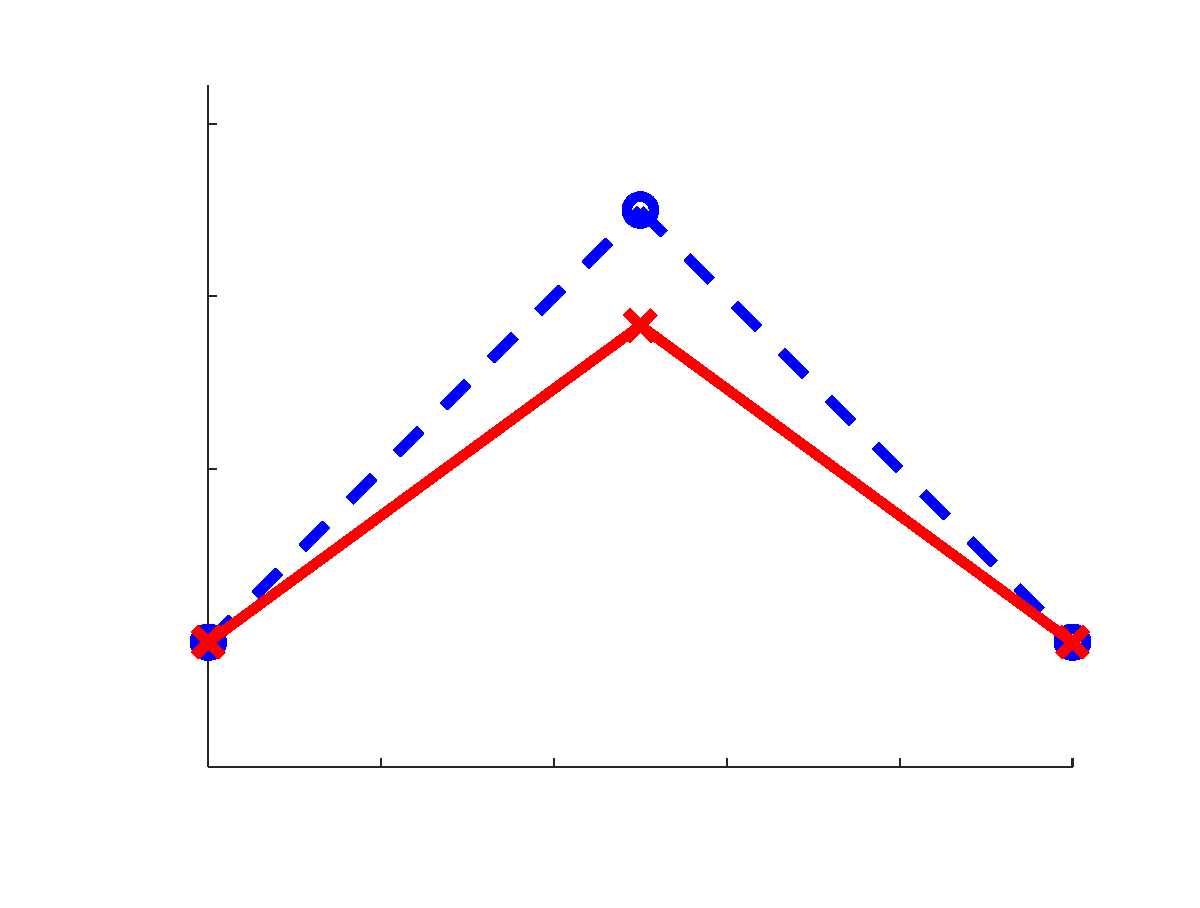
\includegraphics{figmises-inc}
\end{picture}%
\begin{picture}(560,420)(0,0)
\fontsize{22}{0}
\selectfont\put(91.9953,54.728){\makebox(0,0)[t]{\textcolor[rgb]{0.15,0.15,0.15}{{0}}}}
\fontsize{22}{0}
\selectfont\put(174.956,54.728){\makebox(0,0)[t]{\textcolor[rgb]{0.15,0.15,0.15}{{1000}}}}
\fontsize{22}{0}
\selectfont\put(257.917,54.728){\makebox(0,0)[t]{\textcolor[rgb]{0.15,0.15,0.15}{{2000}}}}
\fontsize{22}{0}
\selectfont\put(340.878,54.728){\makebox(0,0)[t]{\textcolor[rgb]{0.15,0.15,0.15}{{3000}}}}
\fontsize{22}{0}
\selectfont\put(423.839,54.728){\makebox(0,0)[t]{\textcolor[rgb]{0.15,0.15,0.15}{{4000}}}}
\fontsize{22}{0}
\selectfont\put(506.8,54.728){\makebox(0,0)[t]{\textcolor[rgb]{0.15,0.15,0.15}{{5000}}}}
\fontsize{22}{0}
\selectfont\put(86.9977,119.61){\makebox(0,0)[r]{\textcolor[rgb]{0.15,0.15,0.15}{{0}}}}
\fontsize{22}{0}
\selectfont\put(86.9977,202.571){\makebox(0,0)[r]{\textcolor[rgb]{0.15,0.15,0.15}{{1000}}}}
\fontsize{22}{0}
\selectfont\put(86.9977,285.531){\makebox(0,0)[r]{\textcolor[rgb]{0.15,0.15,0.15}{{2000}}}}
\fontsize{22}{0}
\selectfont\put(86.9977,368.492){\makebox(0,0)[r]{\textcolor[rgb]{0.15,0.15,0.15}{{3000}}}}
\fontsize{22}{0}
\selectfont\put(299.398,27.7281){\makebox(0,0)[t]{\textcolor[rgb]{0.15,0.15,0.15}{{x}}}}
\fontsize{22}{0}
\selectfont\put(26.9977,223.311){\rotatebox{90}{\makebox(0,0)[b]{\textcolor[rgb]{0.15,0.15,0.15}{{z}}}}}
\end{picture}
}
	\resizebox{.49\linewidth}{!}{% Title: gl2ps_renderer figure
% Creator: GL2PS 1.4.0, (C) 1999-2017 C. Geuzaine
% For: Octave
% CreationDate: Fri Dec 29 11:36:21 2017
\setlength{\unitlength}{1pt}
\begin{picture}(0,0)
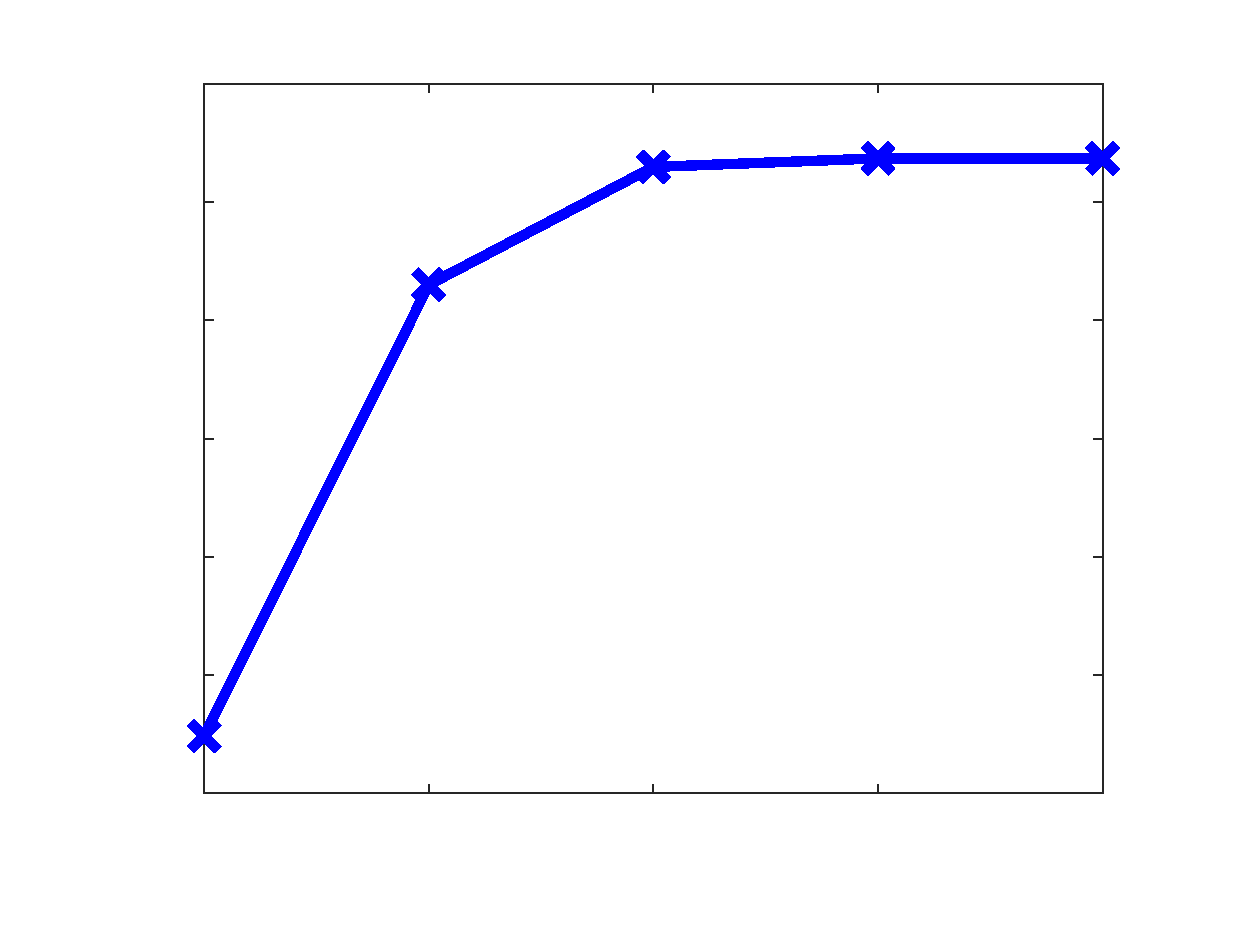
\includegraphics{histukmises-inc}
\end{picture}%
\begin{picture}(576,432)(0,0)
\fontsize{22}{0}
\selectfont\put(89.9966,54.0046){\makebox(0,0)[t]{\textcolor[rgb]{0.15,0.15,0.15}{{1}}}}
\fontsize{22}{0}
\selectfont\put(197.817,54.0046){\makebox(0,0)[t]{\textcolor[rgb]{0.15,0.15,0.15}{{2}}}}
\fontsize{22}{0}
\selectfont\put(305.638,54.0046){\makebox(0,0)[t]{\textcolor[rgb]{0.15,0.15,0.15}{{3}}}}
\fontsize{22}{0}
\selectfont\put(413.459,54.0046){\makebox(0,0)[t]{\textcolor[rgb]{0.15,0.15,0.15}{{4}}}}
\fontsize{22}{0}
\selectfont\put(521.28,54.0046){\makebox(0,0)[t]{\textcolor[rgb]{0.15,0.15,0.15}{{5}}}}
\fontsize{22}{0}
\selectfont\put(84.9933,58.9987){\makebox(0,0)[r]{\textcolor[rgb]{0.15,0.15,0.15}{{400}}}}
\fontsize{22}{0}
\selectfont\put(84.9933,115.766){\makebox(0,0)[r]{\textcolor[rgb]{0.15,0.15,0.15}{{450}}}}
\fontsize{22}{0}
\selectfont\put(84.9933,172.532){\makebox(0,0)[r]{\textcolor[rgb]{0.15,0.15,0.15}{{500}}}}
\fontsize{22}{0}
\selectfont\put(84.9933,229.299){\makebox(0,0)[r]{\textcolor[rgb]{0.15,0.15,0.15}{{550}}}}
\fontsize{22}{0}
\selectfont\put(84.9933,286.066){\makebox(0,0)[r]{\textcolor[rgb]{0.15,0.15,0.15}{{600}}}}
\fontsize{22}{0}
\selectfont\put(84.9933,342.833){\makebox(0,0)[r]{\textcolor[rgb]{0.15,0.15,0.15}{{650}}}}
\fontsize{22}{0}
\selectfont\put(84.9933,399.6){\makebox(0,0)[r]{\textcolor[rgb]{0.15,0.15,0.15}{{700}}}}
\fontsize{22}{0}
\selectfont\put(305.638,27.0046){\makebox(0,0)[t]{\textcolor[rgb]{0.15,0.15,0.15}{{Iteraciones}}}}
\fontsize{22}{0}
\selectfont\put(38.9933,229.299){\rotatebox{90}{\makebox(0,0)[b]{\textcolor[rgb]{0.15,0.15,0.15}{{|$u^k(4)$|}}}}}
\end{picture}
}
	\caption{Resultados de ejecución del Código~\ref{cod:cerchamises}: geometrías de referencia en trazo discontinuo en azul y deformada en rojo continuo (izquierda), gráfico de valores de desplazamiento vertical en cada iteración (derecha).}
	\label{fig:defmises}
\end{figure}

En la Tabla~\ref{tab:resmises} se muestran los resultados obtenidos en cada iteración donde la entrada $4$ del vector $\bfu^k$ contiene el valor de desplazamiento vertical del nodo superior.
%
\begin{table}[htb]
	\centering
	\begin{tabular}{ccccc}
		\hline
		iteración &    $u^{(k)}[4](10^{2})$  &$\varepsilon^{(k)} (10^{-1})$&  $\sigma^{(k)} (10^4)$ & fin? \\ 
		\hline   
		\hline
		1 &   -4.243 &   -0.776 &   -3.883 & 0 \\ 
		2 &   -6.150 &   -1.079 &   -5.394 & 0 \\ 
		3 &   -6.649 &   -1.153 &   -5.765 & 0 \\ 
		4 &   -6.685 &   -1.158 &   -5.791 & 0 \\ 
		5 &   -6.685 &   -1.158 &   -5.791 & 1 \\ 
		\hline
	\end{tabular}
	\caption{Valores obtenidos por el método para el problema de Von Mises.}
	\label{tab:resmises}
\end{table}


Se observa que existe una diferencia relativa de 36 \% entre el valor de desplazamiento obtenido al realizar el análisis lineal y el dado por el análisis no lineal y las tensiones y deformaciones del análisis no lineal tienen mayor magnitud que las del análisis lineal. %
%
Esto es provocado por el hecho de que la estructura pierde considerable rigidez global al deformarse y las barras deben desarrollar mayor tensión para equilibrar la fuerza aplicada. %
%
La deformación axial alcanza el 10\% por lo que se puede considerar que se deja de cumplir la hipótesis de pequeñas deformaciones. %
%
En el análisis de estructuras reales esto es algo importante a verificar.

El código también calcula los errores con respecto a los valores analíticos obtenidos en la sección anterior. En clase se discutirán e interpretarán los resultados así como también se mostrarán variantes de los resultados al modificar los parámetros de la estructura.

\cajaactividad{
	Modificar los parámetros del Código~\ref{cod:cerchamises} para reproducir los resultados presentados en el Ejemplo 1 del artículo \citep{Li2017}.}

\subsubsection{Apoyos elásticos}

Se considera ahora el caso en el que un nodo $j$ de la estructura está vinculado a tierra a través de resortes lineales de constante elástica $k_x$ y $k_y$ según $x$ e $y$, tal como se muestra en la Figura~\ref{fig:apoyoselas}.

\begin{figure}[htb]
	\centering
	\def\svgwidth{0.32\textwidth}
    \input{../fig/Nodo_resorte.pdf_tex}
	\caption{Esquema resortes en nodo $j$.}
	\label{fig:apoyoselas}
\end{figure}

Las fuerzas correspondientes a los resortes pueden ser consideradas como fuerzas externas dadas por:
%
\begin{equation}
f_{\text{ext},s,x} = - u_{j,x} k_x \qquad f_{\text{ext},s,x} = - u_{j,y} k_y .
\end{equation}

Es posible recorrer los resortes de todos los nodos y ensamblar en un vector de fuerzas externas de resortes, el cual dependerá del desplazamiento actual $\bfu^k$ e incluso utilizar una forma matricial:
%
\begin{equation}
\bff_{\text{ext},s} (\bfu) = -\bfK_S \bfu
\end{equation}
donde la matriz $\bfK_S$ tiene las correspondientes constantes elásticas en las entradas de la diagonal. %
%

Este vector de fuerzas externas debidas a los apoyos elásticos puede ser convenientemente considerado como un vector de fuerzas internas
\begin{equation}
\bff_{\text{int},s} (\bfu) = \bfK_S \bfu,
\end{equation}
al considerarlo en el otro miembro de la igualdad de trabajos virtuales. %
%


\cajaactividad{Mostrar que el sistema lineal asociado al método de Newton-Raphson considerando apoyos elásticos está dado por:
	\begin{equation}
	\left(
	  \bfK_{T}(\bfu^{(k)}) + \bfK_{S} 
	\right) \, \Delta \bfu^{(k)} = \bff_{\text{ext}} - \bff_{\text{int}}\left( \bfu^{(k)} \right)
	\end{equation}
}


\subsection{Método de Newton-Raphson Incremental}

Se considera ahora que la estructura es analizada de forma incremental, esto quiere decir que las fuerzas externas son aplicadas de a incrementos en instantes de tiempo $t$. Se considera que las cargas externas varían simplemente de acuerdo a un factor de carga y que no dependen de la geometría deformada de la estructura. %
%
Esta variación de las fuerzas externas es representada a través de un superíndice $t$: 
%
\begin{equation}
\bff_{\text{ext},t} = \lambda_t \bff_{\text{ext}}.
\end{equation}
%
Las cargas son también consideradas como aplicadas de forma estática, o con velocidad de variación pequeña en comparación con la inercia y la cantidad de movimiento de la estructura. %
Es decir que el tiempo identifica los incrementos pero no se considera la dinámica.
% ---------------------------------



\subsubsection{Método Incremental}

El Método Incremental consiste en buscar la solución del PTV correspondiente a las fuerzas $\bff_{\text{ext},t+\Delta t}$ partiendo de la solución correspondiente a $\bff_{\text{ext},t}$. %
%
En la Figura~\ref{fig:esquema_barra_ptv} se muestra un esquema de un elemento de barra en su configuración de referencia y en las posiciones deformada $\bfu_t$ y $\bfu_{t+\Delta t}$.

\begin{figure}[htb]
	\centering
\def\svgwidth{0.65\textwidth}
\input{../fig/ptv_truss.pdf_tex}%
	\caption{Esquema de deformadas incrementales de elemento de barra.}
	\label{fig:esquema_barra_ptv}
\end{figure}

En el Algoritmo~\ref{alg:NR} se muestra un pseudo-código del Método de Newton-Raphson incremental para análisis de reticulados, en el cual se hace uso del algoritmo presentado en la sección anterior. %
%
\begin{algorithm}[htb]	
	\caption{Método Newton Raphson incremental para reticulados.}
	\label{alg:NR}
	\begin{algorithmic}[1]
		\WHILE{$t<t_{max}$}
		\STATE Calcular: $\bff_{\text{ext},t+\Delta t}$
		\STATE Actualizar: $\bfu_0 \leftarrow \bfu_t$ y $\bff_{\text{ext}} \leftarrow \bff_{\text{ext},t+\Delta t}$
		\STATE Resolver: Algoritmo~\ref{alg:mefnl1carga} 
		\STATE Actualizar: $\bfu_{t+\Delta t} \leftarrow \bfu_k$
		\STATE Actualizar: $t \leftarrow t+\Delta t$
		\ENDWHILE		
	\end{algorithmic}
\end{algorithm}
%
El método permite obtener las soluciones de equilibrio para cada valor de fuerza considerado, sin embargo presenta limitaciones para obtener soluciones aceptables para valores de carga de puntos límite. %

\subsubsection{Ejemplo de análisis de punto límite}

Se considera el problema de la cercha de Von Mises, abordado en la Sección~\ref{sec:implem}, y se resuelve aplicando el Método Incremental implementado en el código ONSAS. %
%
Como valor de fuerza final aplicada se considera $9\times 10^6$ con $50$ incrementos de carga. %
%
A la izquierda en la Figura~\ref{fig:woodvonmises} se muestra un gráfico generado por el ONSAS con la estructura en la configuración deformada para carga final (trazo rojo grueso) y en la configuración de referencia (trazo azul fino). A la derecha en la misma figura se ve el gráfico de la curva carga-desplazamiento. %

\begin{figure}[htb!]
	\centering
	\resizebox{.46\linewidth}{!}{% Title: gl2ps_renderer figure
% Creator: GL2PS 1.4.0, (C) 1999-2017 C. Geuzaine
% For: Octave
% CreationDate: Fri Dec 29 10:31:06 2017
\setlength{\unitlength}{1pt}
\begin{picture}(0,0)
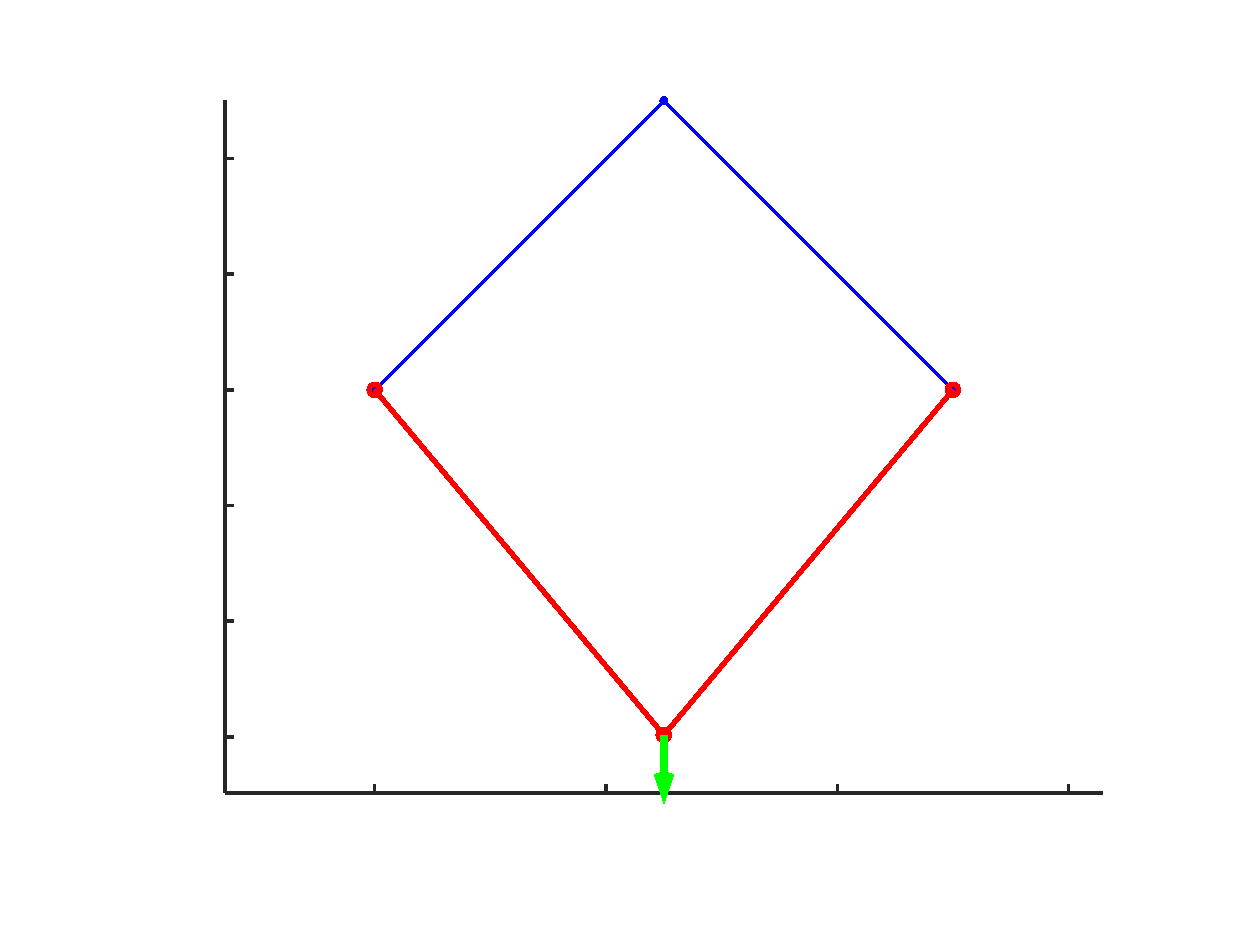
\includegraphics{VonMises_cap2_deform-inc}
\end{picture}%
\begin{picture}(576,432)(0,0)
\fontsize{22}{0}
\selectfont\put(171.868,54.214){\makebox(0,0)[t]{\textcolor[rgb]{0.15,0.15,0.15}{{0}}}}
\fontsize{22}{0}
\selectfont\put(282.888,54.214){\makebox(0,0)[t]{\textcolor[rgb]{0.15,0.15,0.15}{{2000}}}}
\fontsize{22}{0}
\selectfont\put(393.907,54.214){\makebox(0,0)[t]{\textcolor[rgb]{0.15,0.15,0.15}{{4000}}}}
\fontsize{22}{0}
\selectfont\put(504.926,54.214){\makebox(0,0)[t]{\textcolor[rgb]{0.15,0.15,0.15}{{6000}}}}
\fontsize{22}{0}
\selectfont\put(95.0018,86.1786){\makebox(0,0)[r]{\textcolor[rgb]{0.15,0.15,0.15}{{-3000}}}}
\fontsize{22}{0}
\selectfont\put(95.0018,141.688){\makebox(0,0)[r]{\textcolor[rgb]{0.15,0.15,0.15}{{-2000}}}}
\fontsize{22}{0}
\selectfont\put(95.0018,197.198){\makebox(0,0)[r]{\textcolor[rgb]{0.15,0.15,0.15}{{-1000}}}}
\fontsize{22}{0}
\selectfont\put(95.0018,252.708){\makebox(0,0)[r]{\textcolor[rgb]{0.15,0.15,0.15}{{0}}}}
\fontsize{22}{0}
\selectfont\put(95.0018,308.217){\makebox(0,0)[r]{\textcolor[rgb]{0.15,0.15,0.15}{{1000}}}}
\fontsize{22}{0}
\selectfont\put(95.0018,363.727){\makebox(0,0)[r]{\textcolor[rgb]{0.15,0.15,0.15}{{2000}}}}
\fontsize{22}{0}
\selectfont\put(310.643,27.214){\makebox(0,0)[t]{\textcolor[rgb]{0.15,0.15,0.15}{{x}}}}
\fontsize{22}{0}
\selectfont\put(27.0018,225.35){\rotatebox{90}{\makebox(0,0)[b]{\textcolor[rgb]{0.15,0.15,0.15}{{y}}}}}
\end{picture}
}
	\resizebox{.46\linewidth}{!}{% Title: gl2ps_renderer figure
% Creator: GL2PS 1.4.0, (C) 1999-2017 C. Geuzaine
% For: Octave
% CreationDate: Thu Dec 28 13:02:40 2017
\setlength{\unitlength}{1pt}
\begin{picture}(0,0)
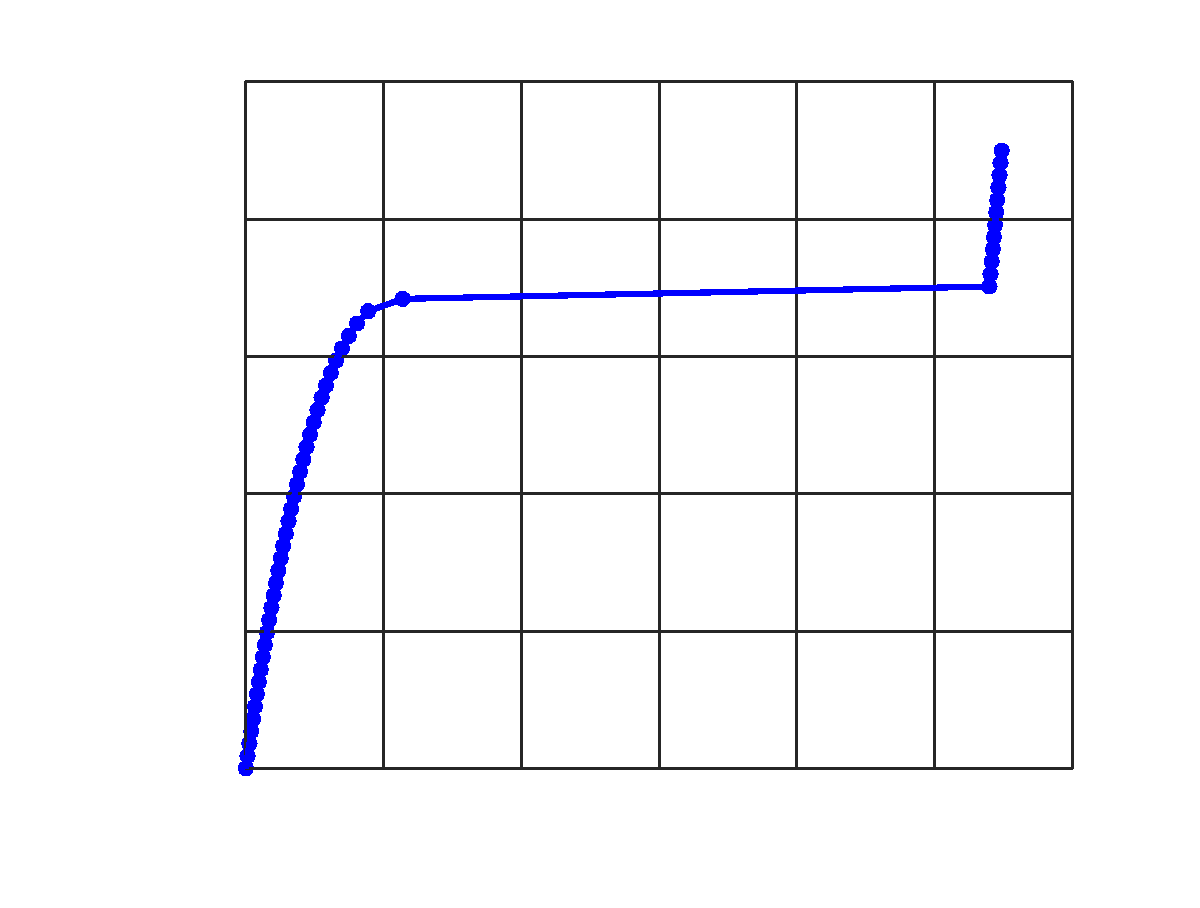
\includegraphics{VonMises_cap2-inc}
\end{picture}%
\begin{picture}(560,420)(0,0)
\fontsize{22}{0}
\selectfont\put(109.998,53.9945){\makebox(0,0)[t]{\textcolor[rgb]{0.15,0.15,0.15}{{0}}}}
\fontsize{22}{0}
\selectfont\put(176.132,53.9945){\makebox(0,0)[t]{\textcolor[rgb]{0.15,0.15,0.15}{{1000}}}}
\fontsize{22}{0}
\selectfont\put(242.265,53.9945){\makebox(0,0)[t]{\textcolor[rgb]{0.15,0.15,0.15}{{2000}}}}
\fontsize{22}{0}
\selectfont\put(308.399,53.9945){\makebox(0,0)[t]{\textcolor[rgb]{0.15,0.15,0.15}{{3000}}}}
\fontsize{22}{0}
\selectfont\put(374.533,53.9945){\makebox(0,0)[t]{\textcolor[rgb]{0.15,0.15,0.15}{{4000}}}}
\fontsize{22}{0}
\selectfont\put(440.666,53.9945){\makebox(0,0)[t]{\textcolor[rgb]{0.15,0.15,0.15}{{5000}}}}
\fontsize{22}{0}
\selectfont\put(506.8,53.9945){\makebox(0,0)[t]{\textcolor[rgb]{0.15,0.15,0.15}{{6000}}}}
\fontsize{22}{0}
\selectfont\put(105.001,59.0021){\makebox(0,0)[r]{\textcolor[rgb]{0.15,0.15,0.15}{{0}}}}
\fontsize{22}{0}
\selectfont\put(105.001,124.902){\makebox(0,0)[r]{\textcolor[rgb]{0.15,0.15,0.15}{{2e+06}}}}
\fontsize{22}{0}
\selectfont\put(105.001,190.801){\makebox(0,0)[r]{\textcolor[rgb]{0.15,0.15,0.15}{{4e+06}}}}
\fontsize{22}{0}
\selectfont\put(105.001,256.701){\makebox(0,0)[r]{\textcolor[rgb]{0.15,0.15,0.15}{{6e+06}}}}
\fontsize{22}{0}
\selectfont\put(105.001,322.6){\makebox(0,0)[r]{\textcolor[rgb]{0.15,0.15,0.15}{{8e+06}}}}
\fontsize{22}{0}
\selectfont\put(105.001,388.5){\makebox(0,0)[r]{\textcolor[rgb]{0.15,0.15,0.15}{{1e+07}}}}
\fontsize{22}{0}
\selectfont\put(308.399,26.9945){\makebox(0,0)[t]{\textcolor[rgb]{0.15,0.15,0.15}{{Displacements}}}}
\fontsize{22}{0}
\selectfont\put(27.0007,223.751){\rotatebox{90}{\makebox(0,0)[b]{\textcolor[rgb]{0.15,0.15,0.15}{{Load factors}}}}}
\end{picture}
}
	\caption{Gráficos obtenidos por el ONSAS al resolver una cercha de Von Mises.}
	\label{fig:woodvonmises}
\end{figure}

Se observa que luego de superado un cierto valor de carga (punto límite) se produce un \textit{salto} en los desplazamientos hacia la rama derecha en el gráfico. %
%
Esto no es una transición continua de las configuraciones de la estructura por lo que el método no es capaz de obtener el comportamiento completo de la estructura para un intervalo de fuerzas. %
%
En la sección siguiente se estudiarán las causas del fenómeno del salto. %
%
Este salto no está provocado por el pandeo local de las barras, fenómeno que no fue considerado en este análisis.

%
Lo mencionado anteriormente representa una limitación considerable del método si se desea realizar un análisis para grandes desplazamientos de una estructura con comportamiento de punto límite. %
%
Para poder obtener la curva completa de desplazamientos es necesario utilizar otras técnicas avanzadas que serán brevemente descritas a continuación.


\subsection{Otras técnicas avanzadas}

\subsubsection{Métodos de Newton-Raphson Modificados y búsquedas lineales}

Tal como se mostró en la Sección~\ref{sec:NRcap1} es posible obtener convergencia a la solución sin la necesidad de calcular la matriz tangente en cada iteración. %
%
El concepto del método de Newton-Raphson modificado es fácilmente aplicable al análisis de elementos finitos visto en la sección anterior, por ejemplo definiendo que la linea 4 del Algoritmo~\ref{alg:mefnl1carga} es realizada cada cierto número de iteraciones. %

En la Sección~\ref{sec:ptvestdef} se mostró que en el caso de estructuras conservativas, el planteo del PTV es equivalente al Principio de Mínima Energía Potencial Total. %
%
El problema de minimización del funcional de energía potencial total puede ser abordado utilizando un amplio importante conjunto de algoritmos para optimización no lineal, como métodos Quasi-Newton o de Búsqueda Lineal, que mejoran considerablemente la eficiencia de los procedimientos numéricos. %
%
A pesar de que algunos de estos métodos están basados en técnicas numéricas de varias décadas, el desarrollo de métodos eficientes de análisis no lineal de estructuras continúa siendo un área de interés científico en la actualidad \citep{Magisano2017}.
% --------------------------------------------------


\subsubsection{Métodos de Longitud de arco}

En el ejemplo de la sección anterior se mostró que el método NR no es capaz de obtener todas las configuraciones de equilibrio intermedio en casos particulares. %
%
El Método de Longitud de Arco introducido en la Sección~\ref{ArcLength} puede ser extendido para la formulación del Método de Elementos Finitos presentada en la sección anterior, permitiendo resolver una más amplia gama de problemas. %
%
Se puede encontrar una implementación completa y didáctica del método en \citep{DeSouzaNeto2008}. %
%
Este método está implementado en el código ONSAS. %

Si el ejemplo de la sección anterior es resuelto usando el código ONSAS con el método de longitud de arco, se obtiene la gráfica mostrada en la Figura~\ref{fig:misesarclen}, donde el incremento de desplazamiento establecido para cada paso de carga es de $70$ y se realizan 100 pasos de carga.
%
\begin{figure}[htb]
	\centering
	\resizebox{.45\linewidth}{!}{% Title: gl2ps_renderer figure
% Creator: GL2PS 1.4.0, (C) 1999-2017 C. Geuzaine
% For: Octave
% CreationDate: Fri Dec 29 10:31:18 2017
\setlength{\unitlength}{1pt}
\begin{picture}(0,0)
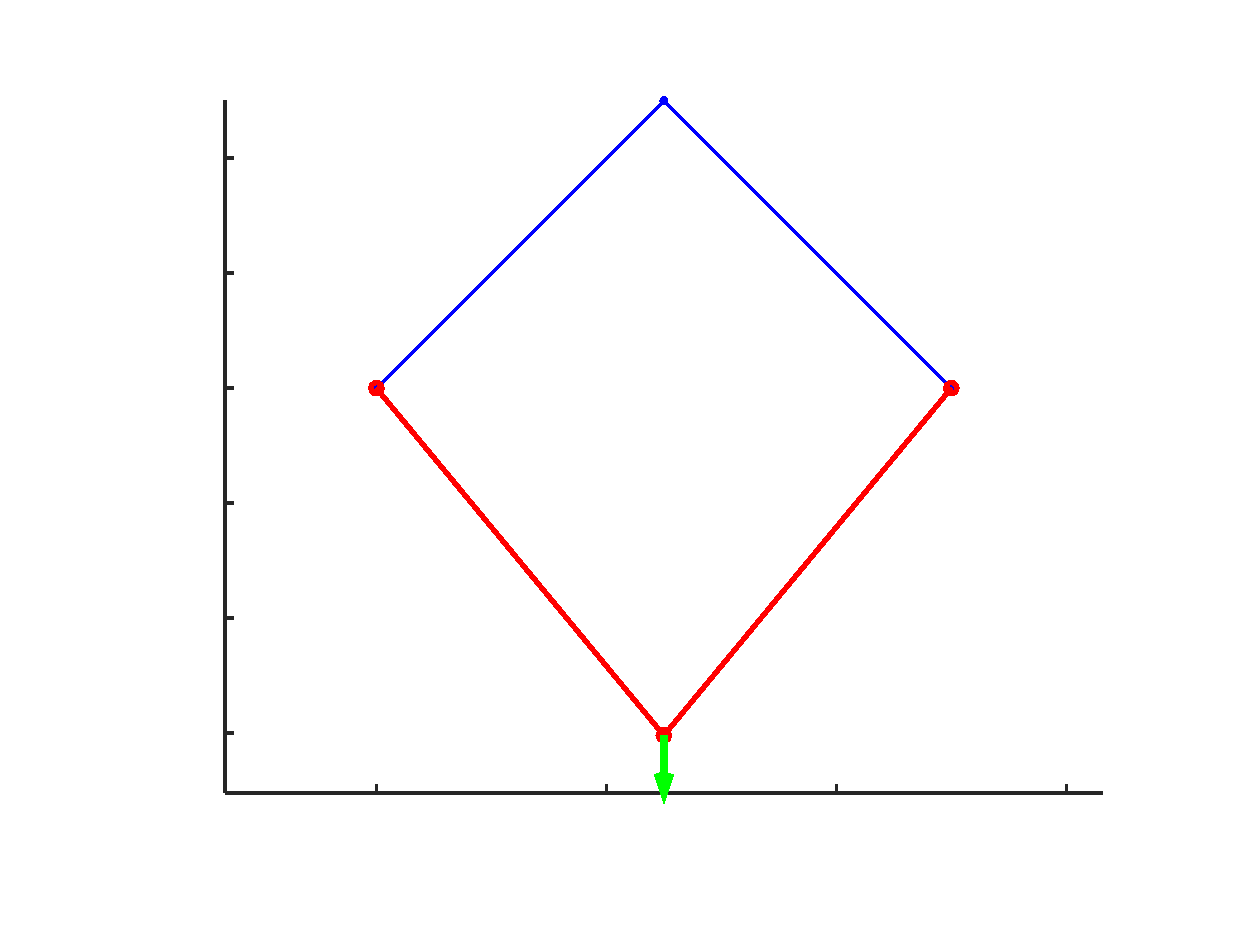
\includegraphics{VonMises_cap2AL_deform-inc}
\end{picture}%
\begin{picture}(576,432)(0,0)
\fontsize{22}{0}
\selectfont\put(172.659,54.214){\makebox(0,0)[t]{\textcolor[rgb]{0.15,0.15,0.15}{{0}}}}
\fontsize{22}{0}
\selectfont\put(283.046,54.214){\makebox(0,0)[t]{\textcolor[rgb]{0.15,0.15,0.15}{{2000}}}}
\fontsize{22}{0}
\selectfont\put(393.432,54.214){\makebox(0,0)[t]{\textcolor[rgb]{0.15,0.15,0.15}{{4000}}}}
\fontsize{22}{0}
\selectfont\put(503.819,54.214){\makebox(0,0)[t]{\textcolor[rgb]{0.15,0.15,0.15}{{6000}}}}
\fontsize{22}{0}
\selectfont\put(95.0018,87.9185){\makebox(0,0)[r]{\textcolor[rgb]{0.15,0.15,0.15}{{-3000}}}}
\fontsize{22}{0}
\selectfont\put(95.0018,143.112){\makebox(0,0)[r]{\textcolor[rgb]{0.15,0.15,0.15}{{-2000}}}}
\fontsize{22}{0}
\selectfont\put(95.0018,198.305){\makebox(0,0)[r]{\textcolor[rgb]{0.15,0.15,0.15}{{-1000}}}}
\fontsize{22}{0}
\selectfont\put(95.0018,253.498){\makebox(0,0)[r]{\textcolor[rgb]{0.15,0.15,0.15}{{0}}}}
\fontsize{22}{0}
\selectfont\put(95.0018,308.692){\makebox(0,0)[r]{\textcolor[rgb]{0.15,0.15,0.15}{{1000}}}}
\fontsize{22}{0}
\selectfont\put(95.0018,363.885){\makebox(0,0)[r]{\textcolor[rgb]{0.15,0.15,0.15}{{2000}}}}
\fontsize{22}{0}
\selectfont\put(310.643,27.214){\makebox(0,0)[t]{\textcolor[rgb]{0.15,0.15,0.15}{{x}}}}
\fontsize{22}{0}
\selectfont\put(27.0018,225.35){\rotatebox{90}{\makebox(0,0)[b]{\textcolor[rgb]{0.15,0.15,0.15}{{y}}}}}
\end{picture}
}
	\resizebox{.45\linewidth}{!}{% Title: gl2ps_renderer figure
% Creator: GL2PS 1.4.0, (C) 1999-2017 C. Geuzaine
% For: Octave
% CreationDate: Thu Dec 28 13:04:17 2017
\setlength{\unitlength}{1pt}
\begin{picture}(0,0)
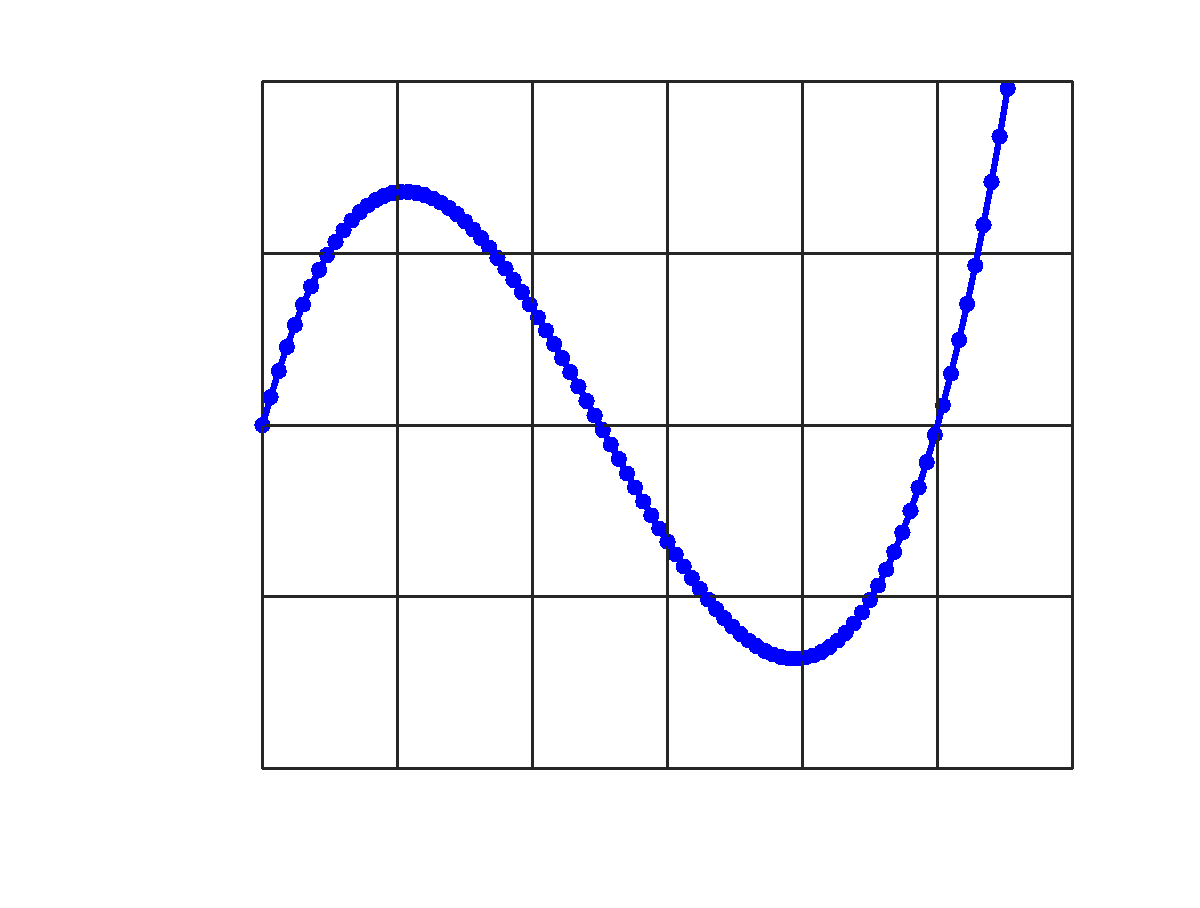
\includegraphics{VonMises_cap2AL-inc}
\end{picture}%
\begin{picture}(560,420)(0,0)
\fontsize{22}{0}
\selectfont\put(118.001,53.9945){\makebox(0,0)[t]{\textcolor[rgb]{0.15,0.15,0.15}{{0}}}}
\fontsize{22}{0}
\selectfont\put(182.801,53.9945){\makebox(0,0)[t]{\textcolor[rgb]{0.15,0.15,0.15}{{1000}}}}
\fontsize{22}{0}
\selectfont\put(247.601,53.9945){\makebox(0,0)[t]{\textcolor[rgb]{0.15,0.15,0.15}{{2000}}}}
\fontsize{22}{0}
\selectfont\put(312.401,53.9945){\makebox(0,0)[t]{\textcolor[rgb]{0.15,0.15,0.15}{{3000}}}}
\fontsize{22}{0}
\selectfont\put(377.2,53.9945){\makebox(0,0)[t]{\textcolor[rgb]{0.15,0.15,0.15}{{4000}}}}
\fontsize{22}{0}
\selectfont\put(442,53.9945){\makebox(0,0)[t]{\textcolor[rgb]{0.15,0.15,0.15}{{5000}}}}
\fontsize{22}{0}
\selectfont\put(506.8,53.9945){\makebox(0,0)[t]{\textcolor[rgb]{0.15,0.15,0.15}{{6000}}}}
\fontsize{22}{0}
\selectfont\put(113.004,59.0021){\makebox(0,0)[r]{\textcolor[rgb]{0.15,0.15,0.15}{{-1e+07}}}}
\fontsize{22}{0}
\selectfont\put(113.004,141.377){\makebox(0,0)[r]{\textcolor[rgb]{0.15,0.15,0.15}{{-5e+06}}}}
\fontsize{22}{0}
\selectfont\put(113.004,223.751){\makebox(0,0)[r]{\textcolor[rgb]{0.15,0.15,0.15}{{0}}}}
\fontsize{22}{0}
\selectfont\put(113.004,306.126){\makebox(0,0)[r]{\textcolor[rgb]{0.15,0.15,0.15}{{5e+06}}}}
\fontsize{22}{0}
\selectfont\put(113.004,388.5){\makebox(0,0)[r]{\textcolor[rgb]{0.15,0.15,0.15}{{1e+07}}}}
\fontsize{22}{0}
\selectfont\put(312.401,26.9945){\makebox(0,0)[t]{\textcolor[rgb]{0.15,0.15,0.15}{{Displacements}}}}
\fontsize{22}{0}
\selectfont\put(27.0036,223.751){\rotatebox{90}{\makebox(0,0)[b]{\textcolor[rgb]{0.15,0.15,0.15}{{Load factors}}}}}
\end{picture}
}
	\caption{Ejemplo de cercha de Von Mises usando método de longitud de arco.}
	\label{fig:misesarclen}
\end{figure}

Se observa cómo este método permite obtener las fuerzas de equilibrio correspondientes a cada configuración intermedia del movimiento de la estructura. %
%

Es importante destacar que los gráficos carga-desplazamiento generados por la versión actual del ONSAS no presentan los segmentos de puntos de equilibrio inestable punteados como se mostró al inicio del capítulo. %
%


\subsection{Ejemplo: Arco bi-articulado} \label{sec:ejarco}

Los arcos han sido utilizados desde la antigüedad en estructuras de gran relevancia como por ejemplo el \textit{Pont du Gard}, estructura que sostiene un acueducto construido por los romanos hace casi 2000 años y que sigue en pié al día de hoy \citep{Timoshenko1953}. %
%
En la actualidad los arcos o estructuras con geometría de arco suelen ser utilizadas en soluciones originales de estructuras de puentes o como soporte de cubiertas de grandes luces. %
%
Frecuentemente se plantean soluciones con esbelteces considerables volviendo necesario considerar deformaciones de segundo orden. %


En la Figura~\ref{fig:retiro} se muestra un ejemplo de un arco reticulado utilizado como soporte del techo de la estación de Retiro en Buenos Aires, Argentina. %
%
\begin{figure}[htb]
	\centering
	\includegraphics[width=\textwidth]{../fig/arcos_retiro}
	\caption{Estación de trenes de Retiro, Buenos Aires, Argentina (foto: JPZ).}
	\label{fig:retiro}
\end{figure}
%
Se puede observar que la estructura consiste en un reticulado y el arco tiene sección transversal de altura decreciente hacia la clave.

En esta sección se considera una estructura de arco simplificada con el objetivo de mostrar el comportamiento observado en este tipo de estructuras. %
%
Se pueden encontrar diversos ejemplos de este tipo en la literatura (ver Sección~6.8.2 de \citep{Bathe2014} o Sección~2.5 de \citep{Crisfield1997}).

En esta sección se considera un arco perfecto simétrico formado por un reticulado hiperestático, con condiciones de apoyo y cargas similares a las de uno de los ejemplos considerados en \citep{timoshenko2012theory}. %
%
La carga distribuida es radial y unitaria. %
%
El área de cada barra es $A=0.4 \text{m} \times 0.01 \text{m} = 4\times 10^{-3} \text{m}^2$ y el módulo de Young es $E=210 $ GPa.
%
Cada nodo extremo está apoyado (articulado) fijo. %
%

Para la resolución se utiliza la herramienta ONSAS realizando el análisis con el Método de Longitud de Arco. %
%
Se puede encontrar el archivo de entrada para este análisis en la Sección~\ref{sec:ejarcoonsas}.


En la Figura~\ref{fig:arcocarga1} se muestran gráficos generados por el ONSAS para un valor de factor de carga correspondiente a una configuración cercana a la del punto límite. %
%
El desplazamiento considerado para la curva carga-desplazamiento es el desplazamiento vertical (positivo hacia abajo) de la clave del arco.

\begin{figure}[htb]
	\centering
	\resizebox{.47\linewidth}{!}{% Title: gl2ps_renderer figure
% Creator: GL2PS 1.4.0, (C) 1999-2017 C. Geuzaine
% For: Octave
% CreationDate: Thu Dec 28 10:36:11 2017
\setlength{\unitlength}{1pt}
\begin{picture}(0,0)
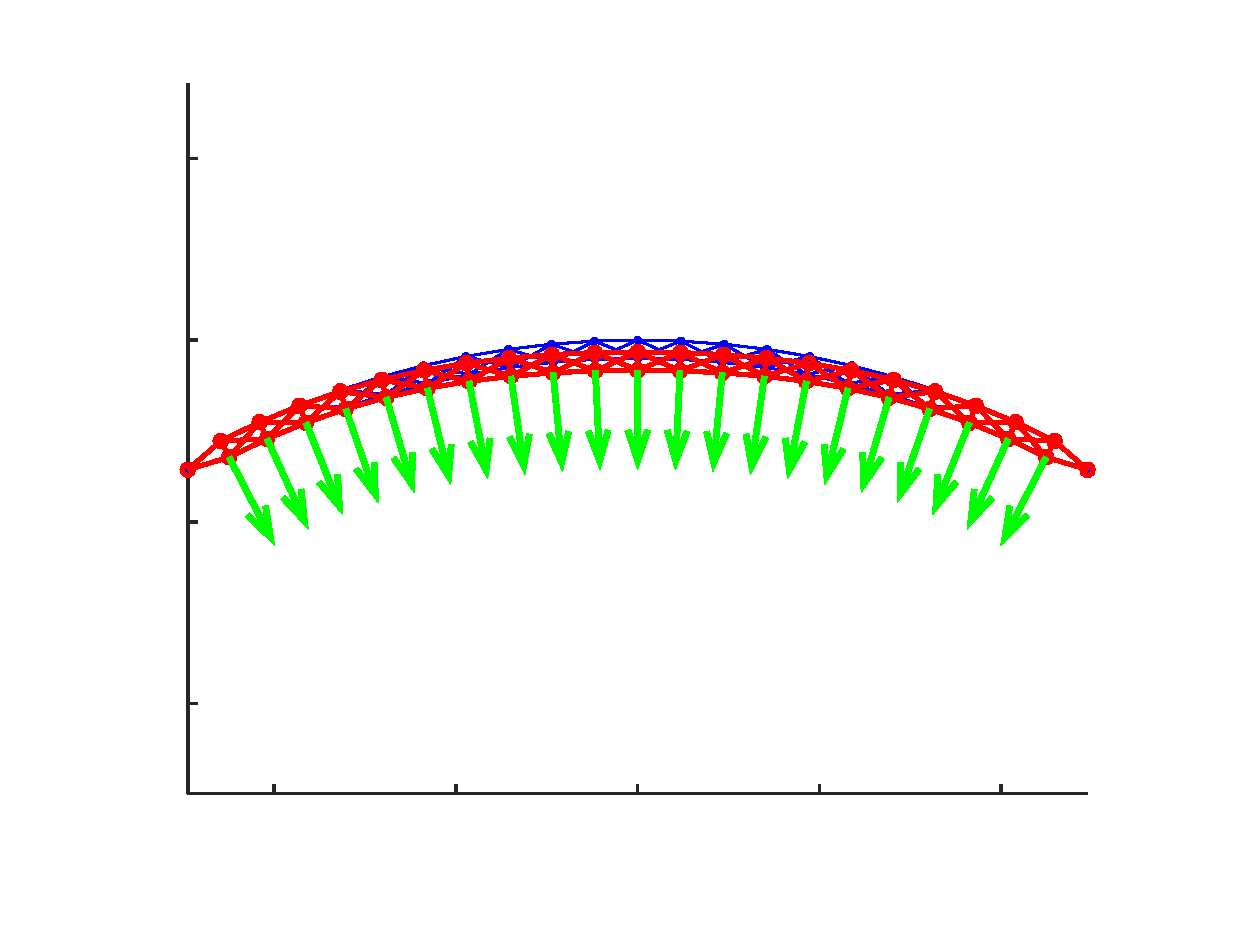
\includegraphics{Pinned_Circular_Arch_perf1_deform-inc}
\end{picture}%
\begin{picture}(576,432)(0,0)
\fontsize{22}{0}
\selectfont\put(123.597,54.0045){\makebox(0,0)[t]{\textcolor[rgb]{0.15,0.15,0.15}{{-20}}}}
\fontsize{22}{0}
\selectfont\put(210.838,54.0045){\makebox(0,0)[t]{\textcolor[rgb]{0.15,0.15,0.15}{{-10}}}}
\fontsize{22}{0}
\selectfont\put(298.08,54.0045){\makebox(0,0)[t]{\textcolor[rgb]{0.15,0.15,0.15}{{0}}}}
\fontsize{22}{0}
\selectfont\put(385.322,54.0045){\makebox(0,0)[t]{\textcolor[rgb]{0.15,0.15,0.15}{{10}}}}
\fontsize{22}{0}
\selectfont\put(472.563,54.0045){\makebox(0,0)[t]{\textcolor[rgb]{0.15,0.15,0.15}{{20}}}}
\fontsize{22}{0}
\selectfont\put(77.1587,102.117){\makebox(0,0)[r]{\textcolor[rgb]{0.15,0.15,0.15}{{30}}}}
\fontsize{22}{0}
\selectfont\put(77.1587,189.359){\makebox(0,0)[r]{\textcolor[rgb]{0.15,0.15,0.15}{{40}}}}
\fontsize{22}{0}
\selectfont\put(77.1587,276.601){\makebox(0,0)[r]{\textcolor[rgb]{0.15,0.15,0.15}{{50}}}}
\fontsize{22}{0}
\selectfont\put(77.1587,363.842){\makebox(0,0)[r]{\textcolor[rgb]{0.15,0.15,0.15}{{60}}}}
\fontsize{22}{0}
\selectfont\put(298.08,27.0045){\makebox(0,0)[t]{\textcolor[rgb]{0.15,0.15,0.15}{{x}}}}
\fontsize{22}{0}
\selectfont\put(45.1587,229.299){\rotatebox{90}{\makebox(0,0)[b]{\textcolor[rgb]{0.15,0.15,0.15}{{y}}}}}
\end{picture}
}
	\resizebox{.47\linewidth}{!}{% Title: gl2ps_renderer figure
% Creator: GL2PS 1.4.0, (C) 1999-2017 C. Geuzaine
% For: Octave
% CreationDate: Thu Dec 28 10:36:12 2017
\setlength{\unitlength}{1pt}
\begin{picture}(0,0)
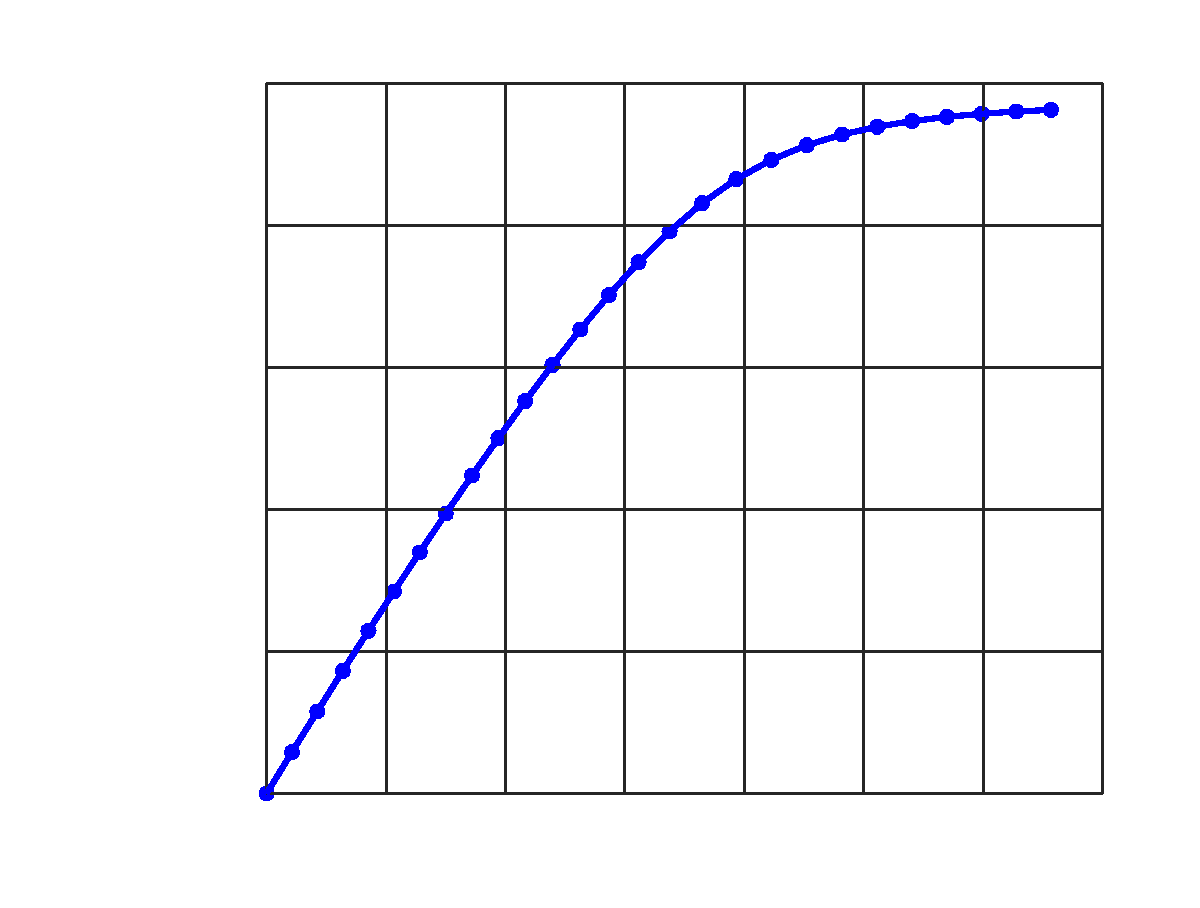
\includegraphics{Pinned_Circular_Arch_perf1-inc}
\end{picture}%
\begin{picture}(560,420)(0,0)
\fontsize{22}{0}
\selectfont\put(119.998,42.0045){\makebox(0,0)[t]{\textcolor[rgb]{0.15,0.15,0.15}{{0}}}}
\fontsize{22}{0}
\selectfont\put(177.324,42.0045){\makebox(0,0)[t]{\textcolor[rgb]{0.15,0.15,0.15}{{0.1}}}}
\fontsize{22}{0}
\selectfont\put(234.65,42.0045){\makebox(0,0)[t]{\textcolor[rgb]{0.15,0.15,0.15}{{0.2}}}}
\fontsize{22}{0}
\selectfont\put(291.976,42.0045){\makebox(0,0)[t]{\textcolor[rgb]{0.15,0.15,0.15}{{0.3}}}}
\fontsize{22}{0}
\selectfont\put(349.302,42.0045){\makebox(0,0)[t]{\textcolor[rgb]{0.15,0.15,0.15}{{0.4}}}}
\fontsize{22}{0}
\selectfont\put(406.628,42.0045){\makebox(0,0)[t]{\textcolor[rgb]{0.15,0.15,0.15}{{0.5}}}}
\fontsize{22}{0}
\selectfont\put(463.954,42.0045){\makebox(0,0)[t]{\textcolor[rgb]{0.15,0.15,0.15}{{0.6}}}}
\fontsize{22}{0}
\selectfont\put(521.28,42.0045){\makebox(0,0)[t]{\textcolor[rgb]{0.15,0.15,0.15}{{0.7}}}}
\fontsize{22}{0}
\selectfont\put(114.995,46.9987){\makebox(0,0)[r]{\textcolor[rgb]{0.15,0.15,0.15}{{0}}}}
\fontsize{22}{0}
\selectfont\put(114.995,115.119){\makebox(0,0)[r]{\textcolor[rgb]{0.15,0.15,0.15}{{50000}}}}
\fontsize{22}{0}
\selectfont\put(114.995,183.239){\makebox(0,0)[r]{\textcolor[rgb]{0.15,0.15,0.15}{{100000}}}}
\fontsize{22}{0}
\selectfont\put(114.995,251.359){\makebox(0,0)[r]{\textcolor[rgb]{0.15,0.15,0.15}{{150000}}}}
\fontsize{22}{0}
\selectfont\put(114.995,319.48){\makebox(0,0)[r]{\textcolor[rgb]{0.15,0.15,0.15}{{200000}}}}
\fontsize{22}{0}
\selectfont\put(114.995,387.6){\makebox(0,0)[r]{\textcolor[rgb]{0.15,0.15,0.15}{{250000}}}}
\fontsize{22}{0}
\selectfont\put(320.639,15.0045){\makebox(0,0)[t]{\textcolor[rgb]{0.15,0.15,0.15}{{Displacements}}}}
\fontsize{22}{0}
\selectfont\put(26.9946,217.299){\rotatebox{90}{\makebox(0,0)[b]{\textcolor[rgb]{0.15,0.15,0.15}{{Load factors}}}}}
\end{picture}
}
	\caption{Gráficos obtenidos en ejemplo de Arco para carga de punto límite.}
	\label{fig:arcocarga1}
\end{figure}

En la Figura~\ref{fig:arcocarga2} se muestra la geometría deformada luego de ocurrido el fenómeno de snap-through así como también la correspondiente gráfica de carga-desplazamiento. %
%
La configuración de referencia corresponde a la geometría dibujada con trazo fino y azul, mientras que la configuración deformada corresponde al trazo grueso en color rojo con círculos en los nodos.

\begin{figure}[htb]
	\centering
	\resizebox{.47\linewidth}{!}{\input{../fig/Pinned_Circular_Arch_perf2_deform}}
	\resizebox{.47\linewidth}{!}{% Title: gl2ps_renderer figure
% Creator: GL2PS 1.4.0, (C) 1999-2017 C. Geuzaine
% For: Octave
% CreationDate: Thu Dec 28 10:48:15 2017
\setlength{\unitlength}{1pt}
\begin{picture}(0,0)
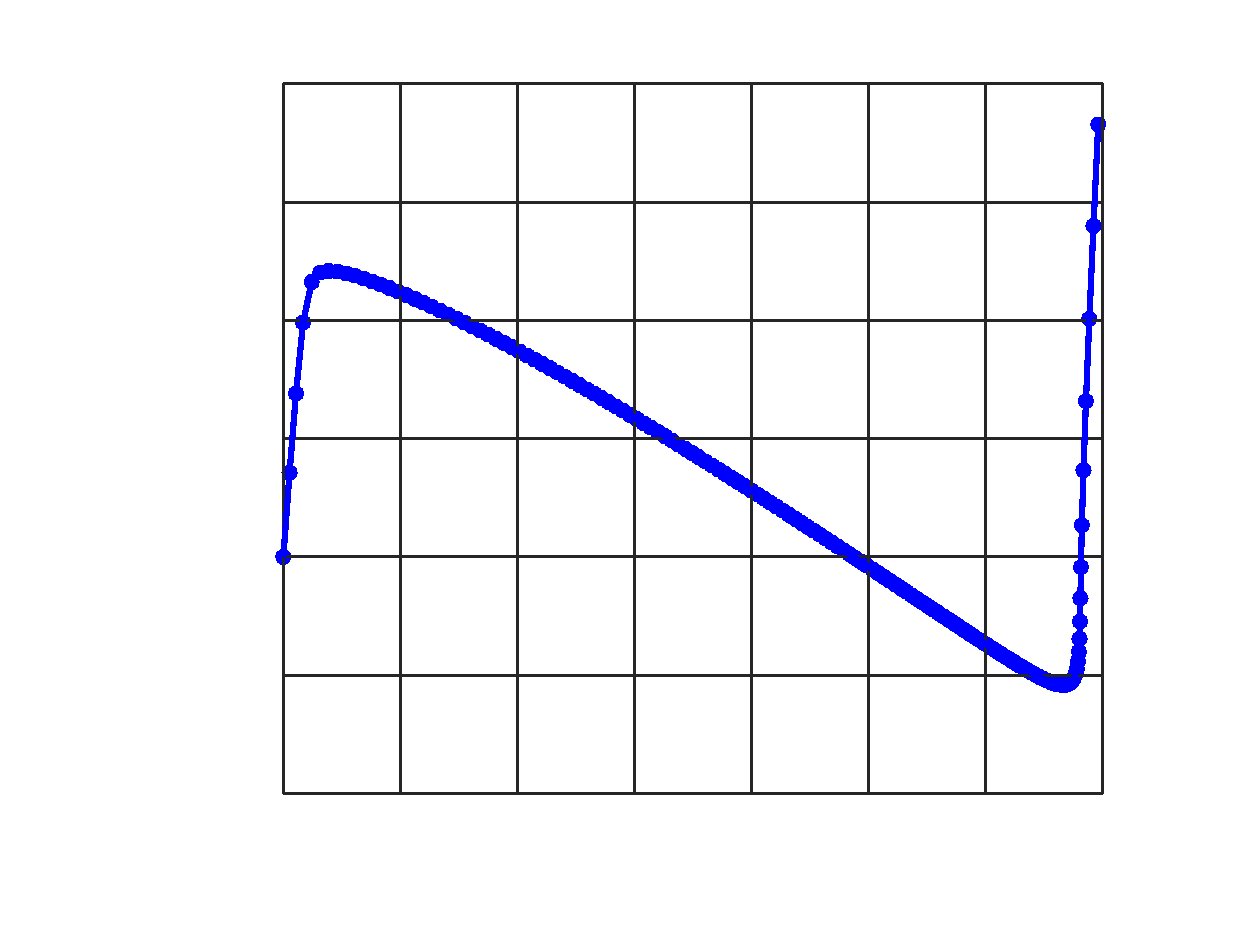
\includegraphics{Pinned_Circular_Arch_perf2-inc}
\end{picture}%
\begin{picture}(576,432)(0,0)
\fontsize{22}{0}
\selectfont\put(127.995,54.0046){\makebox(0,0)[t]{\textcolor[rgb]{0.15,0.15,0.15}{{0}}}}
\fontsize{22}{0}
\selectfont\put(184.179,54.0046){\makebox(0,0)[t]{\textcolor[rgb]{0.15,0.15,0.15}{{2}}}}
\fontsize{22}{0}
\selectfont\put(240.362,54.0046){\makebox(0,0)[t]{\textcolor[rgb]{0.15,0.15,0.15}{{4}}}}
\fontsize{22}{0}
\selectfont\put(296.546,54.0046){\makebox(0,0)[t]{\textcolor[rgb]{0.15,0.15,0.15}{{6}}}}
\fontsize{22}{0}
\selectfont\put(352.729,54.0046){\makebox(0,0)[t]{\textcolor[rgb]{0.15,0.15,0.15}{{8}}}}
\fontsize{22}{0}
\selectfont\put(408.913,54.0046){\makebox(0,0)[t]{\textcolor[rgb]{0.15,0.15,0.15}{{10}}}}
\fontsize{22}{0}
\selectfont\put(465.096,54.0046){\makebox(0,0)[t]{\textcolor[rgb]{0.15,0.15,0.15}{{12}}}}
\fontsize{22}{0}
\selectfont\put(521.28,54.0046){\makebox(0,0)[t]{\textcolor[rgb]{0.15,0.15,0.15}{{14}}}}
\fontsize{22}{0}
\selectfont\put(122.991,58.9987){\makebox(0,0)[r]{\textcolor[rgb]{0.15,0.15,0.15}{{-200000}}}}
\fontsize{22}{0}
\selectfont\put(122.991,115.766){\makebox(0,0)[r]{\textcolor[rgb]{0.15,0.15,0.15}{{-100000}}}}
\fontsize{22}{0}
\selectfont\put(122.991,172.532){\makebox(0,0)[r]{\textcolor[rgb]{0.15,0.15,0.15}{{0}}}}
\fontsize{22}{0}
\selectfont\put(122.991,229.299){\makebox(0,0)[r]{\textcolor[rgb]{0.15,0.15,0.15}{{100000}}}}
\fontsize{22}{0}
\selectfont\put(122.991,286.066){\makebox(0,0)[r]{\textcolor[rgb]{0.15,0.15,0.15}{{200000}}}}
\fontsize{22}{0}
\selectfont\put(122.991,342.833){\makebox(0,0)[r]{\textcolor[rgb]{0.15,0.15,0.15}{{300000}}}}
\fontsize{22}{0}
\selectfont\put(122.991,399.6){\makebox(0,0)[r]{\textcolor[rgb]{0.15,0.15,0.15}{{400000}}}}
\fontsize{22}{0}
\selectfont\put(324.638,27.0046){\makebox(0,0)[t]{\textcolor[rgb]{0.15,0.15,0.15}{{Displacements}}}}
\fontsize{22}{0}
\selectfont\put(26.9915,229.299){\rotatebox{90}{\makebox(0,0)[b]{\textcolor[rgb]{0.15,0.15,0.15}{{Load factors}}}}}
\end{picture}
}
	\caption{Gráficos obtenidos en ejemplo de Arco para carga superior a punto límite.}
	\label{fig:arcocarga2}
\end{figure}

Se observa que la deformación es simétrica tal como se esperaba. %
%
Se puede ver que el máximo valor de factor de carga soportado por la estructura previo al \textit{snap-through} es $\lambda = 2.42 \times 10^5$, sin embargo, hay que destacar que la estructura pierde estabilidad antes de alcanzar dicho factor de carga (esto será visto más adelante). %
%
También se puede verificar que no se supera el $5 \%$ de deformación axial lo que, recordando la Sección~\ref{sec:nlsm}, representa una verificación importante para el modelo y la validez de los resultados usando la medida de deformación de Green y material elástico lineal.

Es de interés observar los gráficos mostrados en la Figura~\ref{fig:arcocarga6}, donde a la izquierda se puede ver la configuración deformada para carga nula, es decir correspondiente al punto de intersección de la curva carga-desplazamiento con la recta $\lambda=0$. La máxima magnitud de deformación axial es $4.71$ \%.
%

\begin{figure}[htb]
	\centering
	\resizebox{.47\linewidth}{!}{% Title: gl2ps_renderer figure
% Creator: GL2PS 1.4.0, (C) 1999-2017 C. Geuzaine
% For: Octave
% CreationDate: Fri Dec 29 10:29:01 2017
\setlength{\unitlength}{1pt}
\begin{picture}(0,0)
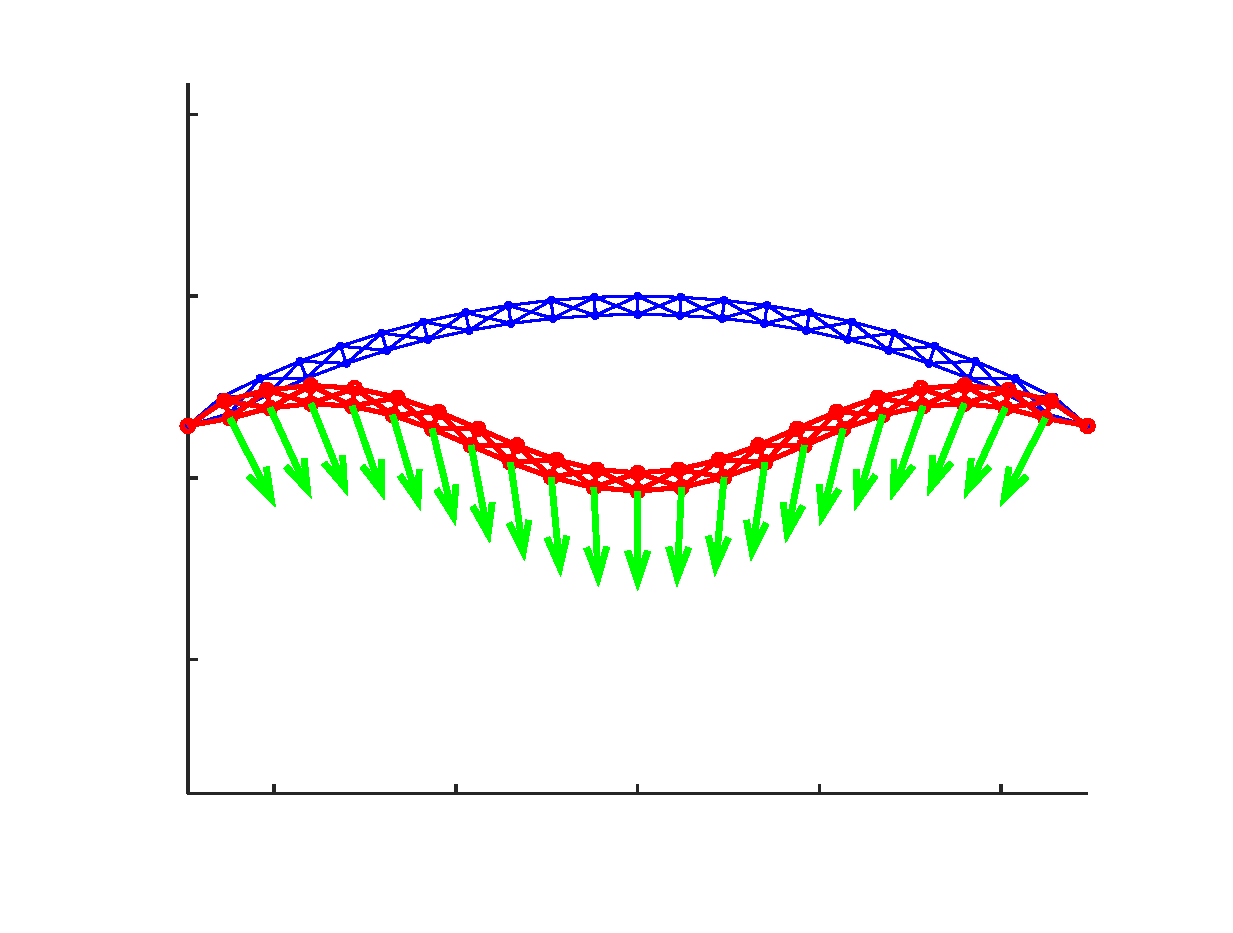
\includegraphics{Pinned_Circular_Arch_perf3_deform-inc}
\end{picture}%
\begin{picture}(576,432)(0,0)
\fontsize{22}{0}
\selectfont\put(123.597,54.0045){\makebox(0,0)[t]{\textcolor[rgb]{0.15,0.15,0.15}{{-20}}}}
\fontsize{22}{0}
\selectfont\put(210.838,54.0045){\makebox(0,0)[t]{\textcolor[rgb]{0.15,0.15,0.15}{{-10}}}}
\fontsize{22}{0}
\selectfont\put(298.08,54.0045){\makebox(0,0)[t]{\textcolor[rgb]{0.15,0.15,0.15}{{0}}}}
\fontsize{22}{0}
\selectfont\put(385.322,54.0045){\makebox(0,0)[t]{\textcolor[rgb]{0.15,0.15,0.15}{{10}}}}
\fontsize{22}{0}
\selectfont\put(472.563,54.0045){\makebox(0,0)[t]{\textcolor[rgb]{0.15,0.15,0.15}{{20}}}}
\fontsize{22}{0}
\selectfont\put(77.1587,123.184){\makebox(0,0)[r]{\textcolor[rgb]{0.15,0.15,0.15}{{30}}}}
\fontsize{22}{0}
\selectfont\put(77.1587,210.425){\makebox(0,0)[r]{\textcolor[rgb]{0.15,0.15,0.15}{{40}}}}
\fontsize{22}{0}
\selectfont\put(77.1587,297.667){\makebox(0,0)[r]{\textcolor[rgb]{0.15,0.15,0.15}{{50}}}}
\fontsize{22}{0}
\selectfont\put(77.1587,384.909){\makebox(0,0)[r]{\textcolor[rgb]{0.15,0.15,0.15}{{60}}}}
\fontsize{22}{0}
\selectfont\put(298.08,27.0045){\makebox(0,0)[t]{\textcolor[rgb]{0.15,0.15,0.15}{{x}}}}
\fontsize{22}{0}
\selectfont\put(45.1587,229.299){\rotatebox{90}{\makebox(0,0)[b]{\textcolor[rgb]{0.15,0.15,0.15}{{y}}}}}
\end{picture}
}
	\resizebox{.47\linewidth}{!}{% Title: gl2ps_renderer figure
% Creator: GL2PS 1.4.0, (C) 1999-2017 C. Geuzaine
% For: Octave
% CreationDate: Thu Dec 28 10:55:01 2017
\setlength{\unitlength}{1pt}
\begin{picture}(0,0)
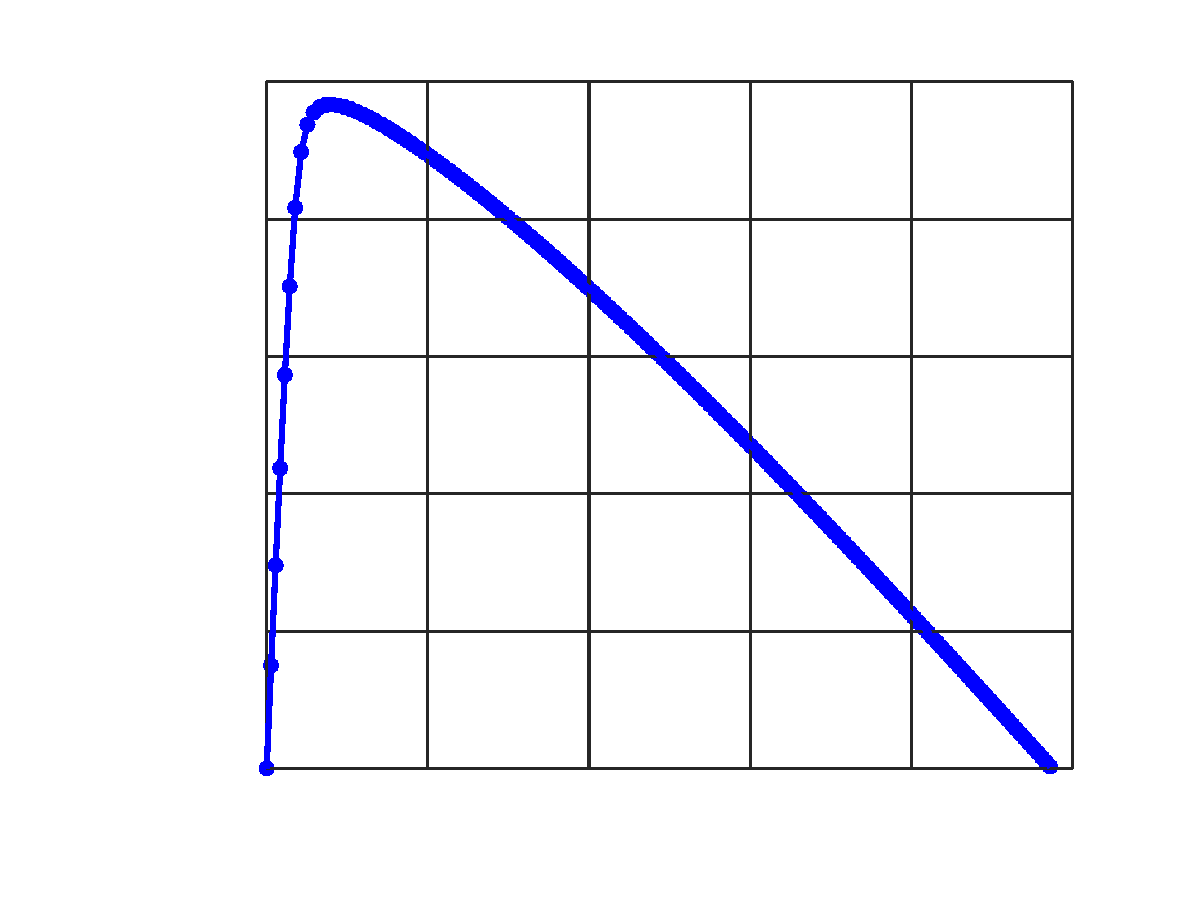
\includegraphics{Pinned_Circular_Arch_perf3-inc}
\end{picture}%
\begin{picture}(560,420)(0,0)
\fontsize{22}{0}
\selectfont\put(120.002,53.9945){\makebox(0,0)[t]{\textcolor[rgb]{0.15,0.15,0.15}{{0}}}}
\fontsize{22}{0}
\selectfont\put(197.361,53.9945){\makebox(0,0)[t]{\textcolor[rgb]{0.15,0.15,0.15}{{2}}}}
\fontsize{22}{0}
\selectfont\put(274.721,53.9945){\makebox(0,0)[t]{\textcolor[rgb]{0.15,0.15,0.15}{{4}}}}
\fontsize{22}{0}
\selectfont\put(352.081,53.9945){\makebox(0,0)[t]{\textcolor[rgb]{0.15,0.15,0.15}{{6}}}}
\fontsize{22}{0}
\selectfont\put(429.44,53.9945){\makebox(0,0)[t]{\textcolor[rgb]{0.15,0.15,0.15}{{8}}}}
\fontsize{22}{0}
\selectfont\put(506.8,53.9945){\makebox(0,0)[t]{\textcolor[rgb]{0.15,0.15,0.15}{{10}}}}
\fontsize{22}{0}
\selectfont\put(115.004,59.0021){\makebox(0,0)[r]{\textcolor[rgb]{0.15,0.15,0.15}{{0}}}}
\fontsize{22}{0}
\selectfont\put(115.004,124.902){\makebox(0,0)[r]{\textcolor[rgb]{0.15,0.15,0.15}{{50000}}}}
\fontsize{22}{0}
\selectfont\put(115.004,190.801){\makebox(0,0)[r]{\textcolor[rgb]{0.15,0.15,0.15}{{100000}}}}
\fontsize{22}{0}
\selectfont\put(115.004,256.701){\makebox(0,0)[r]{\textcolor[rgb]{0.15,0.15,0.15}{{150000}}}}
\fontsize{22}{0}
\selectfont\put(115.004,322.6){\makebox(0,0)[r]{\textcolor[rgb]{0.15,0.15,0.15}{{200000}}}}
\fontsize{22}{0}
\selectfont\put(115.004,388.5){\makebox(0,0)[r]{\textcolor[rgb]{0.15,0.15,0.15}{{250000}}}}
\fontsize{22}{0}
\selectfont\put(313.401,26.9945){\makebox(0,0)[t]{\textcolor[rgb]{0.15,0.15,0.15}{{Displacements}}}}
\fontsize{22}{0}
\selectfont\put(27.0043,223.751){\rotatebox{90}{\makebox(0,0)[b]{\textcolor[rgb]{0.15,0.15,0.15}{{Load factors}}}}}
\end{picture}
}
	\caption{Gráficos obtenidos en ejemplo de Arco para configuración de equilibrio inestable.}
	\label{fig:arcocarga6}
\end{figure}

Esta configuración es claramente inestable ya que cualquier perturbación llevaría a la estructura a adoptar otra configuración. En la siguiente sección se aborda esta temática. %
%

Se observa también que la deformación de la estructura es totalmente simétrica, lo cual está asociado al hecho de que no existen imperfecciones presentes en la geometría de la estructura. La inclusión de imperfecciones en el análisis es algo que brindaría resultados más realistas y será realizado más adelante.


\section{Estabilidad estructural}

La búsqueda de equilibrios inestables es un problema interesante a nivel teórico y fundamentalmente experimental dado que está vinculado a fenómenos de colapso por inestabilidad en estructuras. %
%
Esto atrajo el interés del matemático suizo Leonard Euler, quien a mitad del siglo XVIII publicó su trabajo sobre la carga crítica de una columna, lo que podría considerarse como el primer resultado del Análisis Lineal de Pandeo (o \textit{Linear Buckling Analysis}) \citep{Timoshenko1953}. %
%
Dos siglos después de Euler, científicos de Ingeniería Aeroespacial siguieron trabajando en el estudio del comportamiento de estructuras simples sometidas a compresiones \cite{Huang1971} y más recientemente Ingenieros Estructurales han obtenido resultados originales e interesantes \citep{Bigoni2014,Zaccaria2011}. %
%
Esto denota la importancia que tiene la comprensión de este tipo de fenómenos en estructuras.


En la Sección~\ref{TPE_EQ_STB} se presentaron herramientas útiles para el análisis y clasificación de soluciones de equilibrio de sistemas estructurales. %
%
Para ello se aplicó el Principio de Mínima Energía Potencial, y se formularon las condiciones de mínimo con términos de condiciones sobre el gradiente y la matriz de derivadas segundas de la energía potencial. %

En esta sección se presentan de forma abreviada conceptos básicos para el análisis de estabilidad de sistemas de estructuras reticuladas utilizando la notación matricial de la sección anterior. %
%
Se puede encontrar un desarrollo completo de estos conceptos en el capítulo 9 de \citep{crisfield1996non} o el capítulo 20 de \citep{Crisfield1997}.
% ------------------------------


\subsection{Clasificación de equilibrio}

Sea una estructura cuyos desplazamientos nodales están dados por el vector $\bfu$, la función de energía potencial total está dada por:
%
\begin{equation}
V(\bfu) = U (\bfu) - \bfu^{\text{T}} \bff_{\text{ext}}
\end{equation}
%
donde $U(\bfu)$ es la energía de deformación de toda la estructura y está dada por la suma de las energías de deformación de cada elemento:
%
\begin{equation}
U(\bfu) = \sum_{e=1}^{n_e} \frac{1}{2} A_0 \int_0^{\ell_0^e} \sigma (\bfu^e) \, \varep(\bfu^e) \dif x.
\end{equation}

Si se considera una variación $\delta \bfu$ respecto a la posición asociada a $\bfu$ entonces se puede calcular la variación de la energía potencial correspondiente como:
%
\begin{equation}
\delta V = V ( \bfu + \delta \bfu) - V(\bfu) = U ( \bfu + \delta \bfu) - U(\bfu) - \left( \delta \bfu\right)^{\text{T}} \bff_{\text{ext}}.
\end{equation}
%
Realizando un desarrollo de Taylor de segundo orden de la energía de deformación, y sustituyendo las expresiones de la sección anterior se obtiene que la variación de energía potencial se puede aproximar por:
%
\begin{equation}
\delta V \approx \left( \delta \bfu\right)^{\text{T}}  \left(\bff_{\text{int}}(\bfu) - \bff_{\text{ext}} \right) + \frac{1}{2} ( \delta \bfu)^{\text{T}} \bfK_T(\bfu) \delta \bfu,
\end{equation}
%
donde $\bff_{\text{int}}$ es el vector de fuerzas internas definido en la sección anterior. %
%
Se puede observar que la condición de equilibrio establecida por el principio de trabajos virtuales consiste en anular el término de primer orden de la variación de energía potencial. %


Para poder distinguir diferentes tipos de soluciones de equilibrio se pasa a analizar el término de segundo orden. %
%
Se establece que una configuración dada por $\bfu$ es de \textbf{equilibrio estable} si se cumple el PTV y la energía potencial total aumenta para cualquier perturbación virtual impuesta compatible con los vínculos. %

%
Dado que el signo de la variación de energía potencial está dado por el signo de la forma cuadrática del segundo término, es posible y conveniente establecer las definiciones o clasificaciones de configuraciones de equilibrio en términos de la matriz $\bfK_T$:
%
\begin{itemize}
	\item \textbf{Equilibrio estable}: se dice que la configuración $\bfu$ es de equilibrio estable si $\bfK_T(\bfu)$ es definida positiva, es decir que todos sus valores propios son positivos. %
	%
	Esto es equivalente a la condición
	$$( \delta \bfu)^{\text{T}} \bfK_T(\bfu) \delta \bfu >0 \qquad \forall \delta \bfu.$$ %
	
	\item \textbf{Equilibrio inestable}: se dice que la configuración de equilibro es inestable si se sumple %
	%
	$$( \delta \bfu)^{\text{T}} \bfK_T(\bfu) \delta \bfu \leq 0 \quad \text{ para algún }  \quad \delta \bfu.$$ %
	Esto permite asegurar que la estructura puede adquirir otra configuración de equilibrio, de igual o menor energía potencial, si se realiza una perturbación del equilibrio según $\delta \bfu$. %
	%
\end{itemize}

En los casos de inestabilidad, los vectores propios asociados a los valores propios nulos  de $\bfK_T$ corresponden a los modos de pandeo de la estructura. %
%
Existen otras definiciones o estudios más completos que pueden ser realizados utilizando términos de mayor orden, los cuales no serán abordados en este material.

Es de interés entonces clasificar los equilibrios que se obtienen al resolver un problema de forma incremental. Para eso es posible calcular los valores propios de la matriz tangente asociada a los desplazamientos luego de obtenida la convergencia.
%
La herramienta ONSAS calcula, para cada incremento de carga, los valores propios de la matriz $\bfK_{T}$ mostrando en pantalla la cantidad de valores propios positivos y negativos. %
%

El cálculo de valores propios puede resultar costoso (en el caso de que no se consideren técnicas de factorización particulares en la resolución del sistema lineal \citep{Bathe1982}) y en algunos casos poco eficiente ya que tendrá principal interés para valores de carga cercanos a la inestabilidad, y no necesariamente para valores previos. %

Para estimar los valores de carga de inestabilidad, es posible realizar análisis aproximados de los modos de pandeo. %
%
En las siguientes secciones se presentan y realizan comentarios sobre dos de los métodos aproximados más frecuentemente utilizados.

\subsection{Análisis lineal de pandeo (LBA)}

El análisis lineal de pandeo, también llamado LBA por su sigla en inglés (\textit{Linear Buckling Analysis}), es frecuentemente realizado en la práctica profesional para estimar la carga crítica de pandeo de una estructura y observar sus modos de colapso por inestabilidad (pandeo). %

Se considera una estructura con un estado de fuerzas de referencia $\bff_{\text{ext}}$ y un factor de carga $\lambda \in \bbR$. %
%
Partiendo de la expresión de la matriz tangente, asumiendo que la estructura no se deforma de manera significativa previo a pandear, se desprecian los términos que dependen directamente de $\bfu$ (matriz de desplazamiento inicial)
%
\begin{equation}
\bfK_T (\bfu) = \bfK_{T1} + \bfK_{T2}(\bfu) + \bfK_\sigma(\bfu) \approx \bfK_{T1} + \bfK_\sigma(\bfu).
\end{equation}
%
Respecto a la matriz de tensión inicial se considera una variación proporcional respecto al factor de carga $\sigma = \lambda \bar{\sigma}$, siendo $\bar{\sigma}$ el estado tensional asociado a las fuerzas de referencia $\bff_{\text{ext}}$, es decir para $\lambda=1$. %
%
La matriz aproximada será:
%
\begin{equation}
\bfK_T(\bfu) \approx \left( \bfK_{T1} + \lambda \bar{\bfK}_\sigma \right), 
\end{equation}
donde la matriz $\bar{\bfK}_\sigma$ puede ser fácilmente calculada obteniendo las tensiones de cada elemento mediante un análisis lineal considerando la carga de referencia y realizando el respectivo ensamblado de las matrices elementales. %
% 

El problema de LBA consiste en encontrar el factor de carga correspondiente a un equilibrio inestable utilizando la matriz aproximada. %
%
Esto es equivalente a encontrar los valores $\lambda$ para los cuales la matriz $\bfK_T$ se vuelve singular, es decir que pasa a tener algún valor propio nulo. %
%
Encontrar valor propios nulos de $\bfK_T$ consiste en resolver el siguiente problema

\begin{equation}
\bfK_{T}(\bfu) \bfu = \bszer,
\end{equation}
%
donde sustituyendo la expresión aproximada se puede ver que esto es equivalente a resolver el siguiente problema de valores propios generalizados:
%
\begin{equation}
\bfK_{T1} \bfu = -\lambda \bar{ \bfK_\sigma } \bfu.
\end{equation}

La aproximación realizada sobre la matriz tangente correspondiente a despreciar la matriz de desplazamiento inicial, es equivalente a asumir que la estructura no se deforma considerablemente durante el proceso de carga que la lleva hasta el nivel de carga de pandeo. %
%
En estructuras flexibles que sí se deforman apreciablemente durante el proceso de carga (cáscaras, arcos llanos), esta hipótesis es no conservadora y resulta en estimaciones de la carga de pandeo mayores a la verdadera. Esto puede representar un riesgo si no  es considerado por los métodos de diseño o normativas aplicadas.


\subsection{Análisis no lineal de pandeo}

Es necesario tener en cuenta que para realizar un análisis realista de una estructura se debe poder estimar las cargas vinculadas a los equilibrios inestables de forma suficientemente precisa de forma de garantizar la seguridad de la estructura. %
%
En trabajos como \citep{Wriggers1990} se proponen métodos aproximados para el cálculo de puntos de equilibrio inestable. %
%
Considerando literatura más reciente, se recomienda seguir el abordaje presentado en \citep{Bathe2014} para este tipo de cálculos. %
%
La herramienta ONSAS realiza una estimación de la carga crítica de pandeo para cada valor de factor de carga a través de dicho tipo de análisis aproximado. %
%
El método utilizado también es presentado esquemáticamente en \citep{Li2017}.

\subsection{Ejemplo: Análisis de estabilidad de cercha de Von Mises}

En \citep{Li2017} se aplican ambas técnicas aproximadas de análisis de pandeo a una estructura tipo cercha de Von Mises usando elementos de barra de Green. %
%
En esta sección se presentan los resultados obtenidos al aplicar el código ONSAS a la resolución del problema con los mismos parámetros de dicho ejemplo, se analizan los resultados y se verifican los resultados obtenidos. %
%

En la Tabla~\ref{tab:resnsali} se muestran los resultados obtenidos al resolver el problema usando el código ONSAS. %
%
\begin{table}[htb]
	\centering
	\begin{tabular}{ccccccc}
		\hline
		\#Carga & Factor Carga & Iters & $|\varepsilon|$ (\%) & NonLinBuck  & $\# \lambda>0$ & $\# \lambda\leq0$ \\ 
		\hline
		1 &    1.250e+06  &    4  &  1.34 &  1.67180e+07 &     2 &   0 \\
		2 &    2.500e+06  &    4  &  2.72 &  1.64244e+07 &     2 &   0 \\
		3 &    3.750e+06  &    3  &  4.16 &  1.61137e+07 &     2 &   0 \\
		4 &    5.000e+06  &    3  &  5.66 &  1.57825e+07 &     2 &   0 \\
		5 &    6.250e+06  &    4  &  7.24 &  1.54268e+07 &     2 &   0 \\
		6 &    7.500e+06  &    4  &  8.91 &  1.50413e+07 &     2 &   0 \\
		7 &    8.750e+06  &    4  & 10.69 &  1.46179e+07 &     2 &   0 \\
		8 &    1.000e+07  &    4  & 12.63 &  1.41444e+07 &     2 &   0 \\
		9 &    1.125e+07  &    4  & 14.77 &  1.36000e+07 &     2 &   0 \\
		10 &    1.250e+07  &    4  & 17.25 &  1.29449e+07 &     2 &   0 \\
		11 &    1.375e+07  &    4  & 20.34 &  1.85131e+07 &     1 &   1 \\
		12 &    1.500e+07  &    6  & 26.17 &  1.56950e+07 &     1 &   1 \\
		\hline
	\end{tabular}
	\caption{Resultados obtenidos al resolver el ejemplo de la cercha de Von Mises usando el código ONSAS.}
	\label{tab:resnsali}
\end{table}
%
La columna \textit{Iters} indica la cantidad de iteraciones en desplazamientos realizadas para cada factor de carga. La columna $|\varep|$ indica la  magnitud de la deformación axial en porcentaje, se puede apreciar que se consideran deformaciones superiores a 5 \% aunque esto no evita observar los fenómenos de inestabilidad de interés para el ejemplo. %
%
La columna NonLinBuck muestra el factor de carga de pandeo correspondiente al análisis no lineal. %
%
El código también realiza el análisis lineal y estima la carga de pandeo correspondiente al LBA el cual es $\lambda_L = 1.69966 \times 10^7$. %
%
El archivo de entrada para el ONSAS es presentado en el Código~\ref{cod:inputli2017}.

Se observa que luego de superado el factor de carga número 10, la matriz tangente pasa a tener un valor propio no positivo, esto está dado porque luego del punto de bifurcación se pasa a tener equilibrios inestables. %
%

En la Figura~\ref{fig:grafli} se muestra un gráfico con dos curvas carga desplazamiento una roja con círculos y azul con cruces. Un gráfico similar a este es presentado en el artículo citado. %

\begin{figure}[htb]
	\centering
	\resizebox{.75\linewidth}{!}{% Title: gl2ps_renderer figure
% Creator: GL2PS 1.4.0, (C) 1999-2017 C. Geuzaine
% For: Octave
% CreationDate: Fri Dec 29 11:40:15 2017
\setlength{\unitlength}{1pt}
\begin{picture}(0,0)
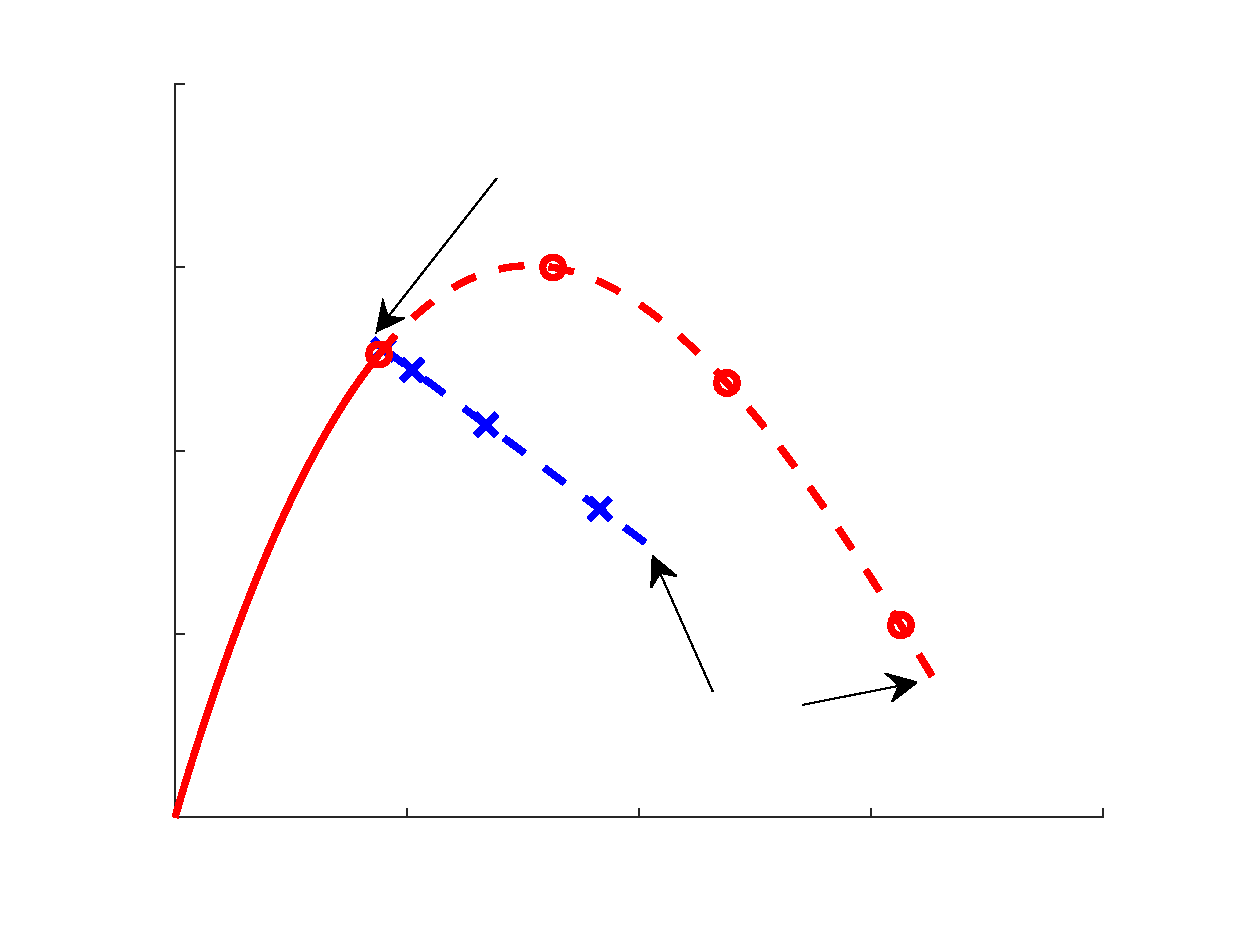
\includegraphics{figli-inc}
\end{picture}%
\begin{picture}(576,432)(0,0)
\fontsize{15}{0}
\selectfont\put(76.0013,42.5189){\makebox(0,0)[t]{\textcolor[rgb]{0.15,0.15,0.15}{{0}}}}
\fontsize{15}{0}
\selectfont\put(187.321,42.5189){\makebox(0,0)[t]{\textcolor[rgb]{0.15,0.15,0.15}{{50}}}}
\fontsize{15}{0}
\selectfont\put(298.641,42.5189){\makebox(0,0)[t]{\textcolor[rgb]{0.15,0.15,0.15}{{100}}}}
\fontsize{15}{0}
\selectfont\put(409.96,42.5189){\makebox(0,0)[t]{\textcolor[rgb]{0.15,0.15,0.15}{{150}}}}
\fontsize{15}{0}
\selectfont\put(521.28,42.5189){\makebox(0,0)[t]{\textcolor[rgb]{0.15,0.15,0.15}{{200}}}}
\fontsize{15}{0}
\selectfont\put(70.9981,47.52){\makebox(0,0)[r]{\textcolor[rgb]{0.15,0.15,0.15}{{0}}}}
\fontsize{15}{0}
\selectfont\put(70.9981,135.54){\makebox(0,0)[r]{\textcolor[rgb]{0.15,0.15,0.15}{{5000}}}}
\fontsize{15}{0}
\selectfont\put(70.9981,223.56){\makebox(0,0)[r]{\textcolor[rgb]{0.15,0.15,0.15}{{10000}}}}
\fontsize{15}{0}
\selectfont\put(70.9981,311.58){\makebox(0,0)[r]{\textcolor[rgb]{0.15,0.15,0.15}{{15000}}}}
\fontsize{15}{0}
\selectfont\put(70.9981,399.6){\makebox(0,0)[r]{\textcolor[rgb]{0.15,0.15,0.15}{{20000}}}}
\fontsize{14}{0}
\selectfont\put(298.641,24.5188){\makebox(0,0)[t]{\textcolor[rgb]{0.15,0.15,0.15}{{Desplazamiento vertical (cm)}}}}
\fontsize{14}{0}
\selectfont\put(16.9981,223.56){\rotatebox{90}{\makebox(0,0)[b]{\textcolor[rgb]{0.15,0.15,0.15}{{Fuerza aplicada (kN)}}}}}
\fontsize{15}{0}
\selectfont\put(275.08,100){\makebox(0,0)[l]{\textcolor[rgb]{0,0,0}{{Ramas inestables}}}}
\fontsize{15}{0}
\selectfont\put(230.4,362.24){\makebox(0,0)[l]{\textcolor[rgb]{0,0,0}{{Punto de bifuraci\'on}}}}
\end{picture}
}
	\caption{Gráfico de curvas carga-desplazamiento para cercha de Von Mises.}
	\label{fig:grafli}
\end{figure}

Se observa que existe un punto de bifurcación entre las dos posibles ramas de equilibrio de la estructura y a partir de dicho punto los puntos de equilibrio corresponden a equilibrios inestables. %
%
Esto es coherente con el resultado visto en la Tabla~\ref{tab:resnsali} donde a partir del décimo factor de carga se obtienen valores propios no nulos de la matriz tangente, correspondiendo esto a la bifurcación y generación de más de una rama de equilibrio.

En estructuras con imperfecciones el proceso de carga lleva a que la estructura adquiera configuraciones recorriendo la rama azul con cruces, por lo que la carga máxima soportada puede ser considerablemente menor que la del punto límite sin considerar imperfecciones. %
La resolución por el método de longitud de arco provoca que se opte por continuar el análisis siguiendo la rama principal o aquella cuya variación del sentido de los desplazamientos sea menor. Para estructuras con imperfecciones, este método es capaz de, para valores adecuados de los parámetros, obtener soluciones en esas ramas de equilibrio. %
%
Se pueden encontrar otros métodos de búsqueda de otras configuraciones o salto entre ramas en \citep{DeSouzaNeto2008,Crisfield1997}.

%
En la Figura~\ref{fig:vonmis} se muestra una configuración obtenida realizando un análisis con el ONSAS considerando una imperfección en la geometría de referencia. %
%
El archivo de entrada del ONSAS es presentado en el Código~\ref{cod:inputli2017imperf}.

\begin{figure}[htb]
	\centering
	\resizebox{.47\linewidth}{!}{% Title: gl2ps_renderer figure
% Creator: GL2PS 1.4.0, (C) 1999-2017 C. Geuzaine
% For: Octave
% CreationDate: Fri Dec 29 10:29:47 2017
\setlength{\unitlength}{1pt}
\begin{picture}(0,0)
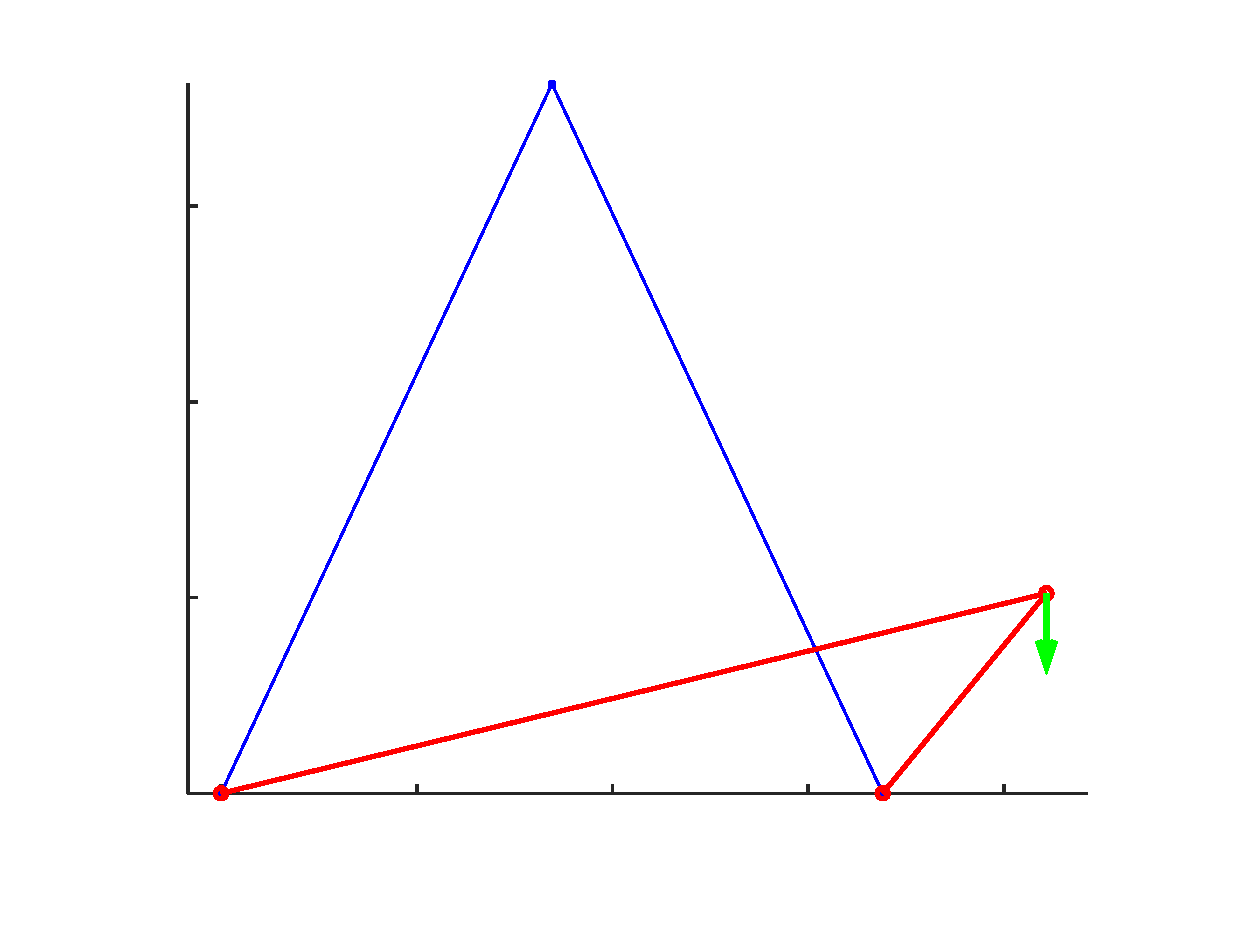
\includegraphics{VonMises_Li2017_imperf_deform-inc}
\end{picture}%
\begin{picture}(576,432)(0,0)
\fontsize{22}{0}
\selectfont\put(98.0882,54.0045){\makebox(0,0)[t]{\textcolor[rgb]{0.15,0.15,0.15}{{0}}}}
\fontsize{22}{0}
\selectfont\put(192.041,54.0045){\makebox(0,0)[t]{\textcolor[rgb]{0.15,0.15,0.15}{{0.5}}}}
\fontsize{22}{0}
\selectfont\put(285.994,54.0045){\makebox(0,0)[t]{\textcolor[rgb]{0.15,0.15,0.15}{{1}}}}
\fontsize{22}{0}
\selectfont\put(379.947,54.0045){\makebox(0,0)[t]{\textcolor[rgb]{0.15,0.15,0.15}{{1.5}}}}
\fontsize{22}{0}
\selectfont\put(473.9,54.0045){\makebox(0,0)[t]{\textcolor[rgb]{0.15,0.15,0.15}{{2}}}}
\fontsize{22}{0}
\selectfont\put(77.1586,58.9986){\makebox(0,0)[r]{\textcolor[rgb]{0.15,0.15,0.15}{{0}}}}
\fontsize{22}{0}
\selectfont\put(77.1586,152.952){\makebox(0,0)[r]{\textcolor[rgb]{0.15,0.15,0.15}{{0.5}}}}
\fontsize{22}{0}
\selectfont\put(77.1586,246.905){\makebox(0,0)[r]{\textcolor[rgb]{0.15,0.15,0.15}{{1}}}}
\fontsize{22}{0}
\selectfont\put(77.1586,340.858){\makebox(0,0)[r]{\textcolor[rgb]{0.15,0.15,0.15}{{1.5}}}}
\fontsize{22}{0}
\selectfont\put(298.08,27.0045){\makebox(0,0)[t]{\textcolor[rgb]{0.15,0.15,0.15}{{x}}}}
\fontsize{22}{0}
\selectfont\put(38.1586,229.299){\rotatebox{90}{\makebox(0,0)[b]{\textcolor[rgb]{0.15,0.15,0.15}{{y}}}}}
\end{picture}
}
	\resizebox{.47\linewidth}{!}{% Title: gl2ps_renderer figure
% Creator: GL2PS 1.4.0, (C) 1999-2017 C. Geuzaine
% For: Octave
% CreationDate: Thu Dec 28 12:29:46 2017
\setlength{\unitlength}{1pt}
\begin{picture}(0,0)
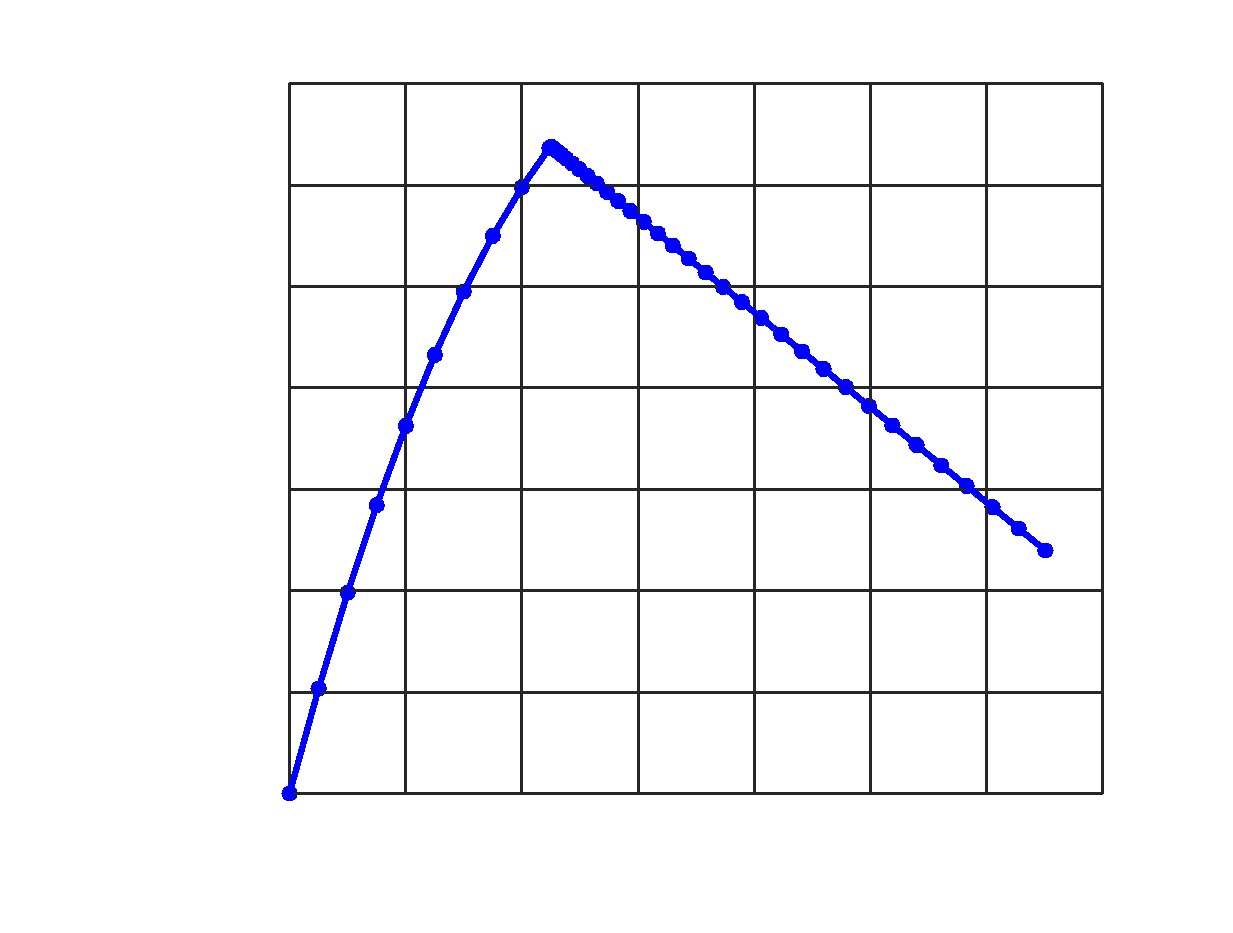
\includegraphics{VonMises_Li2017_imperf-inc}
\end{picture}%
\begin{picture}(576,432)(0,0)
\fontsize{22}{0}
\selectfont\put(130.994,54.0046){\makebox(0,0)[t]{\textcolor[rgb]{0.15,0.15,0.15}{{0}}}}
\fontsize{22}{0}
\selectfont\put(186.749,54.0046){\makebox(0,0)[t]{\textcolor[rgb]{0.15,0.15,0.15}{{0.2}}}}
\fontsize{22}{0}
\selectfont\put(242.504,54.0046){\makebox(0,0)[t]{\textcolor[rgb]{0.15,0.15,0.15}{{0.4}}}}
\fontsize{22}{0}
\selectfont\put(298.259,54.0046){\makebox(0,0)[t]{\textcolor[rgb]{0.15,0.15,0.15}{{0.6}}}}
\fontsize{22}{0}
\selectfont\put(354.015,54.0046){\makebox(0,0)[t]{\textcolor[rgb]{0.15,0.15,0.15}{{0.8}}}}
\fontsize{22}{0}
\selectfont\put(409.77,54.0046){\makebox(0,0)[t]{\textcolor[rgb]{0.15,0.15,0.15}{{1}}}}
\fontsize{22}{0}
\selectfont\put(465.525,54.0046){\makebox(0,0)[t]{\textcolor[rgb]{0.15,0.15,0.15}{{1.2}}}}
\fontsize{22}{0}
\selectfont\put(521.28,54.0046){\makebox(0,0)[t]{\textcolor[rgb]{0.15,0.15,0.15}{{1.4}}}}
\fontsize{22}{0}
\selectfont\put(125.99,58.9987){\makebox(0,0)[r]{\textcolor[rgb]{0.15,0.15,0.15}{{0}}}}
\fontsize{22}{0}
\selectfont\put(125.99,107.656){\makebox(0,0)[r]{\textcolor[rgb]{0.15,0.15,0.15}{{2e+06}}}}
\fontsize{22}{0}
\selectfont\put(125.99,156.313){\makebox(0,0)[r]{\textcolor[rgb]{0.15,0.15,0.15}{{4e+06}}}}
\fontsize{22}{0}
\selectfont\put(125.99,204.971){\makebox(0,0)[r]{\textcolor[rgb]{0.15,0.15,0.15}{{6e+06}}}}
\fontsize{22}{0}
\selectfont\put(125.99,253.628){\makebox(0,0)[r]{\textcolor[rgb]{0.15,0.15,0.15}{{8e+06}}}}
\fontsize{22}{0}
\selectfont\put(125.99,302.285){\makebox(0,0)[r]{\textcolor[rgb]{0.15,0.15,0.15}{{1e+07}}}}
\fontsize{22}{0}
\selectfont\put(125.99,350.943){\makebox(0,0)[r]{\textcolor[rgb]{0.15,0.15,0.15}{{1.2e+07}}}}
\fontsize{22}{0}
\selectfont\put(125.99,399.6){\makebox(0,0)[r]{\textcolor[rgb]{0.15,0.15,0.15}{{1.4e+07}}}}
\fontsize{22}{0}
\selectfont\put(326.137,27.0045){\makebox(0,0)[t]{\textcolor[rgb]{0.15,0.15,0.15}{{Displacements}}}}
\fontsize{22}{0}
\selectfont\put(26.9902,229.299){\rotatebox{90}{\makebox(0,0)[b]{\textcolor[rgb]{0.15,0.15,0.15}{{Load factors}}}}}
\end{picture}
}
	\caption{Gráficos obtenidos para ejemplo de cercha de Von Mises con imperfección.}
	\label{fig:vonmis}
\end{figure}
%
La carga máxima soportada por la estructura es $1.27 \times 10^7$ lo cual coincide con el punto de bifurcación obtenido en el artículo citado.


\subsection{Ejemplo: modo de pandeo asimétrico de arco bi-articulado}

Para finalizar la sección se presentan los elementos básicos del análisis del modo de colapso del arco presentado en la Sección~\ref{sec:ejarco}. %
%
Tal como se vió, al aumentar la carga aplicada al arco se produce una deformación simétrica hasta alcanzar el punto límite provocando el \textit{snap-through}. %
%
Sin embargo en este problema existe un valor de factor de carga menor al del punto límite para el cual se produce un pandeo según un modo no simétrico. %
En \citep{timoshenko2012theory} se presenta el cálculo del valor de carga distribuida crítica
%
\begin{equation}
q_{cr} = \frac{E I}{R^3} \left( \frac{\pi^2}{\alpha^2} -1\right),
\end{equation}
%
donde $R$ es el radio de la circunferencia de la línea media del arco, $E$ el módulo de Young, $I$ la inercia de la sección transversal y $\alpha$ es la mitad del ángulo del arco.
%

A partir del modelo de reticulado se calcula una inercia equivalente $I_{eq}= 2 A (h/2)^2$ donde $A$ es el área de cada barra y fueron consideradas únicamente las áreas de la barras en los extremos superior e inferior de la sección transversal. %
%
Para obtener el valor teórico se asume que el arco es inextensible por lo que una de las posibles fuentes de diferencias con respecto al análisis de reticulados está asociado a la deformación axial por directa.

Los valores de carga crítica de pandeo teórico y obtenidos por el ONSAS mediante análisis de pandeo lineal, no lineal y considerando imperfecciones son mostrados en la Tabla~\ref{tab:pand}. %
%
Las imperfecciones consideradas corresponden a una deformación de la configuración de referencia dada por el primer modo de pandeo lineal de la estructura, con una magnitud máxima del orden de un centímetro.
%
\begin{table}[htb]
	\centering
	\begin{tabular}{l|cc}
		\hline
		Método & Valor $q_{cr}$ $(10^5)$ & Diferencia relativa (\%) \\
		\hline
		\hline
		Valor teórico & 1.212 & 0 \\
		\hline
		LBA ONSAS - Sin imperf. & 1.235 &  1.9 \\
		NonLin ONSAS  - Sin imperf. & 1.206  & -0.5 \\
		\hline
		LBA ONSAS  - Con imperf.& 1.235 & 1.9 \\
		NonLin ONSAS - Con imperf.& 1.186 & -2.1\\
		\hline
	\end{tabular}
	\caption{Valores de carga crítica de pandeo teóricos y numéricos.}
	\label{tab:pand}
\end{table}

El primer comentario importante a realizar es que efectivamente la carga crítica de pandeo es aproximadamente la mitad de la carga del punto de tangente horizontal para la estructura de acuerdo a la deformación simétrica. %
%
Por otra parte se observa que nuevamente la carga crítica del análisis lineal de pandeo es mayor que la carga crítica del análisis no lineal de pandeo.

Para poder observar el modo de colapso por pandeo es necesario considerar imperfecciones geométricas en la estructura y realizar el análisis. %
%
En la Figura~\ref{fig:arcopand} se muestra la deformación posterior al colapso por pandeo así como también la curva carga-desplazamiento.

\begin{figure}[htb]
	\centering
	\resizebox{.47\linewidth}{!}{% Title: gl2ps_renderer figure
% Creator: GL2PS 1.4.0, (C) 1999-2017 C. Geuzaine
% For: Octave
% CreationDate: Fri Dec 29 10:12:54 2017
\setlength{\unitlength}{1pt}
\begin{picture}(0,0)
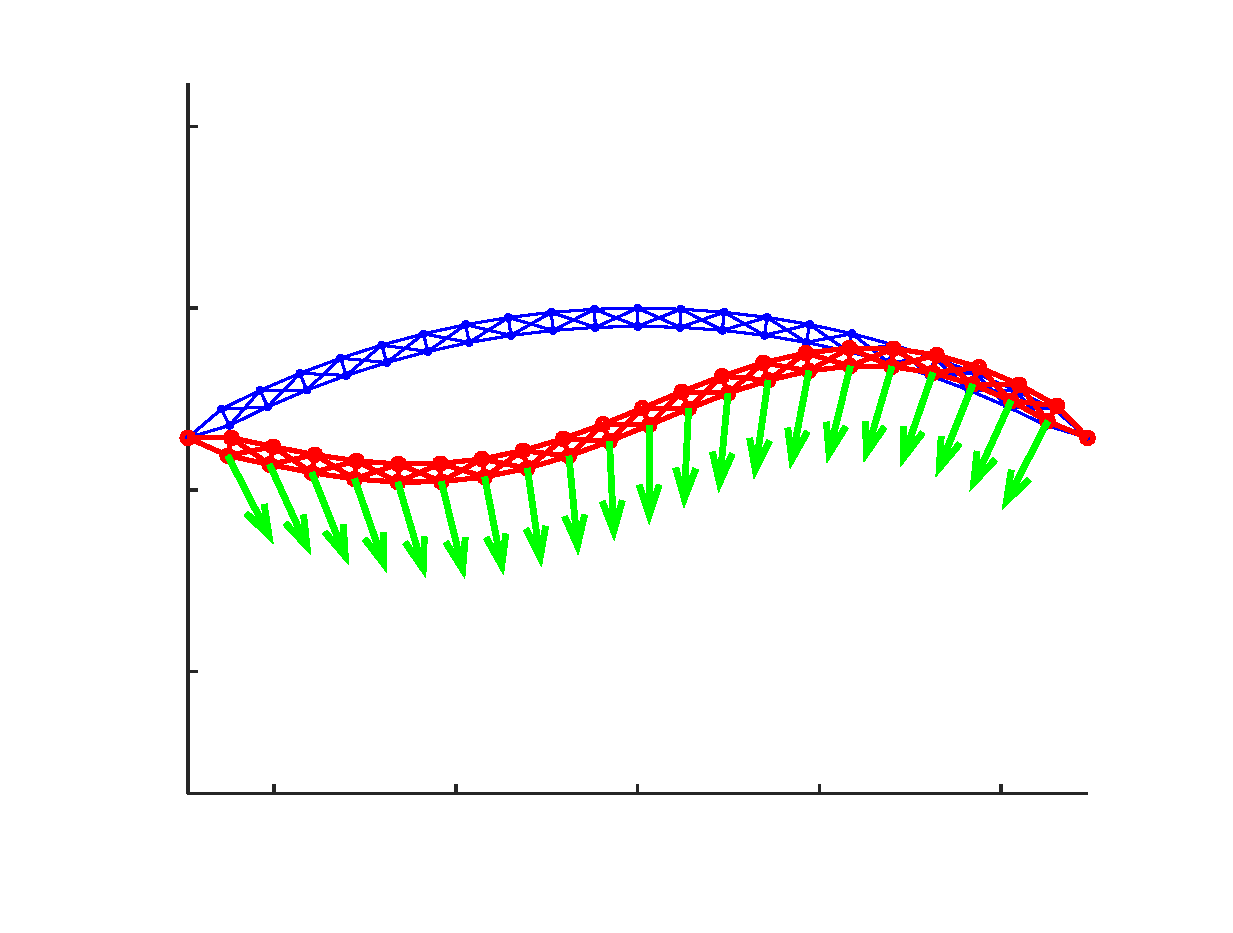
\includegraphics{Pinned_Circular_Arch_imperf_deform-inc}
\end{picture}%
\begin{picture}(576,432)(0,0)
\fontsize{22}{0}
\selectfont\put(123.597,54.0045){\makebox(0,0)[t]{\textcolor[rgb]{0.15,0.15,0.15}{{-20}}}}
\fontsize{22}{0}
\selectfont\put(210.838,54.0045){\makebox(0,0)[t]{\textcolor[rgb]{0.15,0.15,0.15}{{-10}}}}
\fontsize{22}{0}
\selectfont\put(298.08,54.0045){\makebox(0,0)[t]{\textcolor[rgb]{0.15,0.15,0.15}{{0}}}}
\fontsize{22}{0}
\selectfont\put(385.322,54.0045){\makebox(0,0)[t]{\textcolor[rgb]{0.15,0.15,0.15}{{10}}}}
\fontsize{22}{0}
\selectfont\put(472.563,54.0045){\makebox(0,0)[t]{\textcolor[rgb]{0.15,0.15,0.15}{{20}}}}
\fontsize{22}{0}
\selectfont\put(77.1586,117.439){\makebox(0,0)[r]{\textcolor[rgb]{0.15,0.15,0.15}{{30}}}}
\fontsize{22}{0}
\selectfont\put(77.1586,204.681){\makebox(0,0)[r]{\textcolor[rgb]{0.15,0.15,0.15}{{40}}}}
\fontsize{22}{0}
\selectfont\put(77.1586,291.922){\makebox(0,0)[r]{\textcolor[rgb]{0.15,0.15,0.15}{{50}}}}
\fontsize{22}{0}
\selectfont\put(77.1586,379.164){\makebox(0,0)[r]{\textcolor[rgb]{0.15,0.15,0.15}{{60}}}}
\fontsize{22}{0}
\selectfont\put(298.08,27.0045){\makebox(0,0)[t]{\textcolor[rgb]{0.15,0.15,0.15}{{x}}}}
\fontsize{22}{0}
\selectfont\put(45.1586,229.299){\rotatebox{90}{\makebox(0,0)[b]{\textcolor[rgb]{0.15,0.15,0.15}{{y}}}}}
\end{picture}
}
	\resizebox{.47\linewidth}{!}{% Title: gl2ps_renderer figure
% Creator: GL2PS 1.4.0, (C) 1999-2017 C. Geuzaine
% For: Octave
% CreationDate: Fri Dec 29 10:12:57 2017
\setlength{\unitlength}{1pt}
\begin{picture}(0,0)
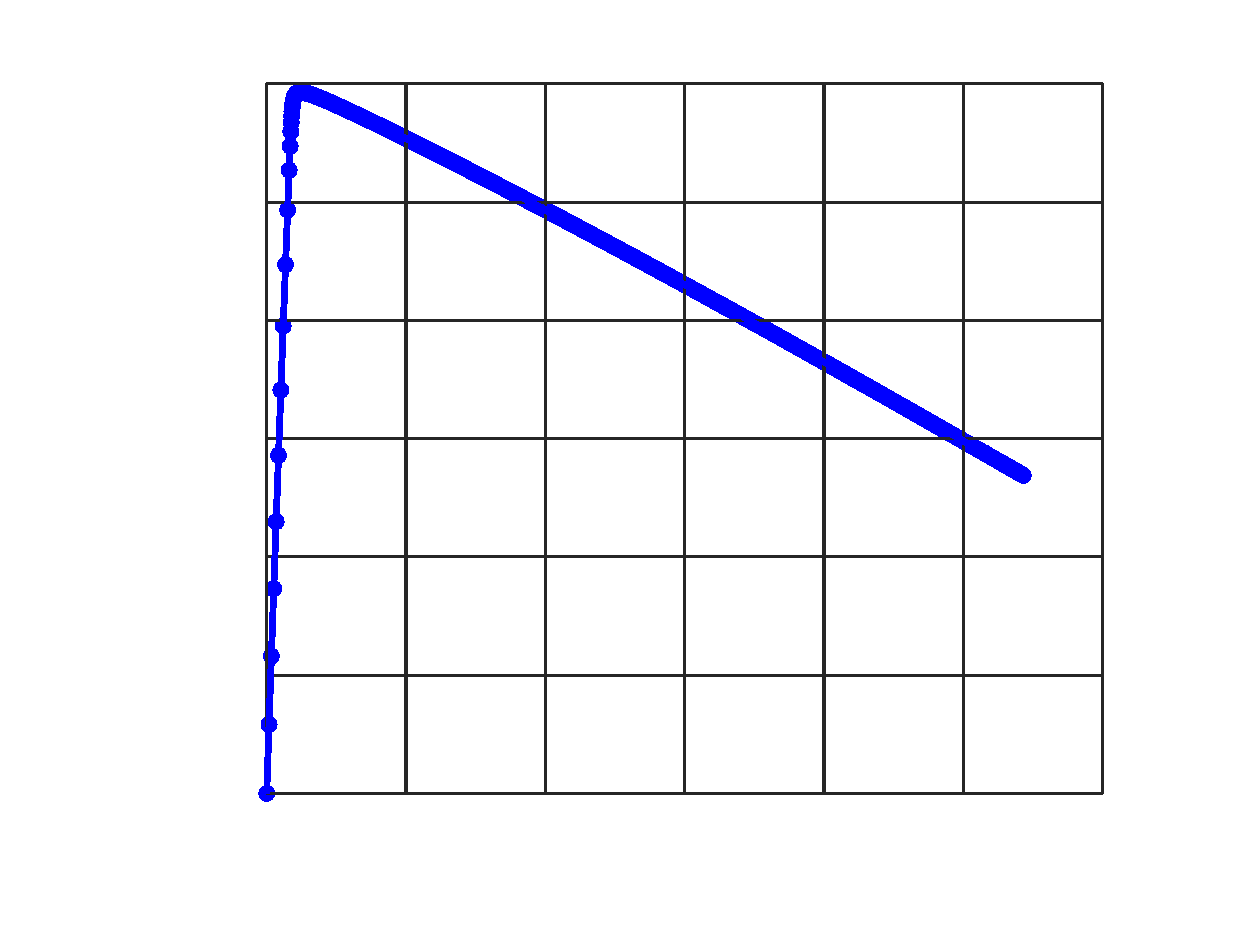
\includegraphics{Pinned_Circular_Arch_imperf-inc}
\end{picture}%
\begin{picture}(576,432)(0,0)
\fontsize{22}{0}
\selectfont\put(119.998,54.0046){\makebox(0,0)[t]{\textcolor[rgb]{0.15,0.15,0.15}{{0}}}}
\fontsize{22}{0}
\selectfont\put(186.878,54.0046){\makebox(0,0)[t]{\textcolor[rgb]{0.15,0.15,0.15}{{1}}}}
\fontsize{22}{0}
\selectfont\put(253.759,54.0046){\makebox(0,0)[t]{\textcolor[rgb]{0.15,0.15,0.15}{{2}}}}
\fontsize{22}{0}
\selectfont\put(320.639,54.0046){\makebox(0,0)[t]{\textcolor[rgb]{0.15,0.15,0.15}{{3}}}}
\fontsize{22}{0}
\selectfont\put(387.519,54.0046){\makebox(0,0)[t]{\textcolor[rgb]{0.15,0.15,0.15}{{4}}}}
\fontsize{22}{0}
\selectfont\put(454.4,54.0046){\makebox(0,0)[t]{\textcolor[rgb]{0.15,0.15,0.15}{{5}}}}
\fontsize{22}{0}
\selectfont\put(521.28,54.0046){\makebox(0,0)[t]{\textcolor[rgb]{0.15,0.15,0.15}{{6}}}}
\fontsize{22}{0}
\selectfont\put(114.995,58.9987){\makebox(0,0)[r]{\textcolor[rgb]{0.15,0.15,0.15}{{0}}}}
\fontsize{22}{0}
\selectfont\put(114.995,115.766){\makebox(0,0)[r]{\textcolor[rgb]{0.15,0.15,0.15}{{20000}}}}
\fontsize{22}{0}
\selectfont\put(114.995,172.532){\makebox(0,0)[r]{\textcolor[rgb]{0.15,0.15,0.15}{{40000}}}}
\fontsize{22}{0}
\selectfont\put(114.995,229.299){\makebox(0,0)[r]{\textcolor[rgb]{0.15,0.15,0.15}{{60000}}}}
\fontsize{22}{0}
\selectfont\put(114.995,286.066){\makebox(0,0)[r]{\textcolor[rgb]{0.15,0.15,0.15}{{80000}}}}
\fontsize{22}{0}
\selectfont\put(114.995,342.833){\makebox(0,0)[r]{\textcolor[rgb]{0.15,0.15,0.15}{{100000}}}}
\fontsize{22}{0}
\selectfont\put(114.995,399.6){\makebox(0,0)[r]{\textcolor[rgb]{0.15,0.15,0.15}{{120000}}}}
\fontsize{22}{0}
\selectfont\put(320.639,27.0046){\makebox(0,0)[t]{\textcolor[rgb]{0.15,0.15,0.15}{{Displacements}}}}
\fontsize{22}{0}
\selectfont\put(26.9946,229.299){\rotatebox{90}{\makebox(0,0)[b]{\textcolor[rgb]{0.15,0.15,0.15}{{Load factors}}}}}
\end{picture}
}
	\caption{Gráficos obtenidos en ejemplo de Arco para configuración de equilibrio inestable.}
	\label{fig:arcopand}
\end{figure}

A través de este ejemplo se muestra la importancia de realizar este tipo de análisis para la determinación de cargas críticas de forma adecuada.

Para finalizar el capítulo se destaca que en estructuras como puentes, los arcos pueden ser utilizados como soporte del tablero, conectado a través de cables. %
%
En la Figura~\ref{fig:arcobridge} se muestra un modelo simplificado de un puente formado por un arco, el tablero y cables (sin resistencia a compresión) que los conectan, donde las cargas son aplicadas en el tablero en lugar del arco. %
%
\begin{figure}[htb]
	\centering
	\resizebox{.55\linewidth}{!}{% Title: gl2ps_renderer figure
% Creator: GL2PS 1.4.0, (C) 1999-2017 C. Geuzaine
% For: Octave
% CreationDate: Fri Dec 29 10:10:51 2017
\setlength{\unitlength}{1pt}
\begin{picture}(0,0)
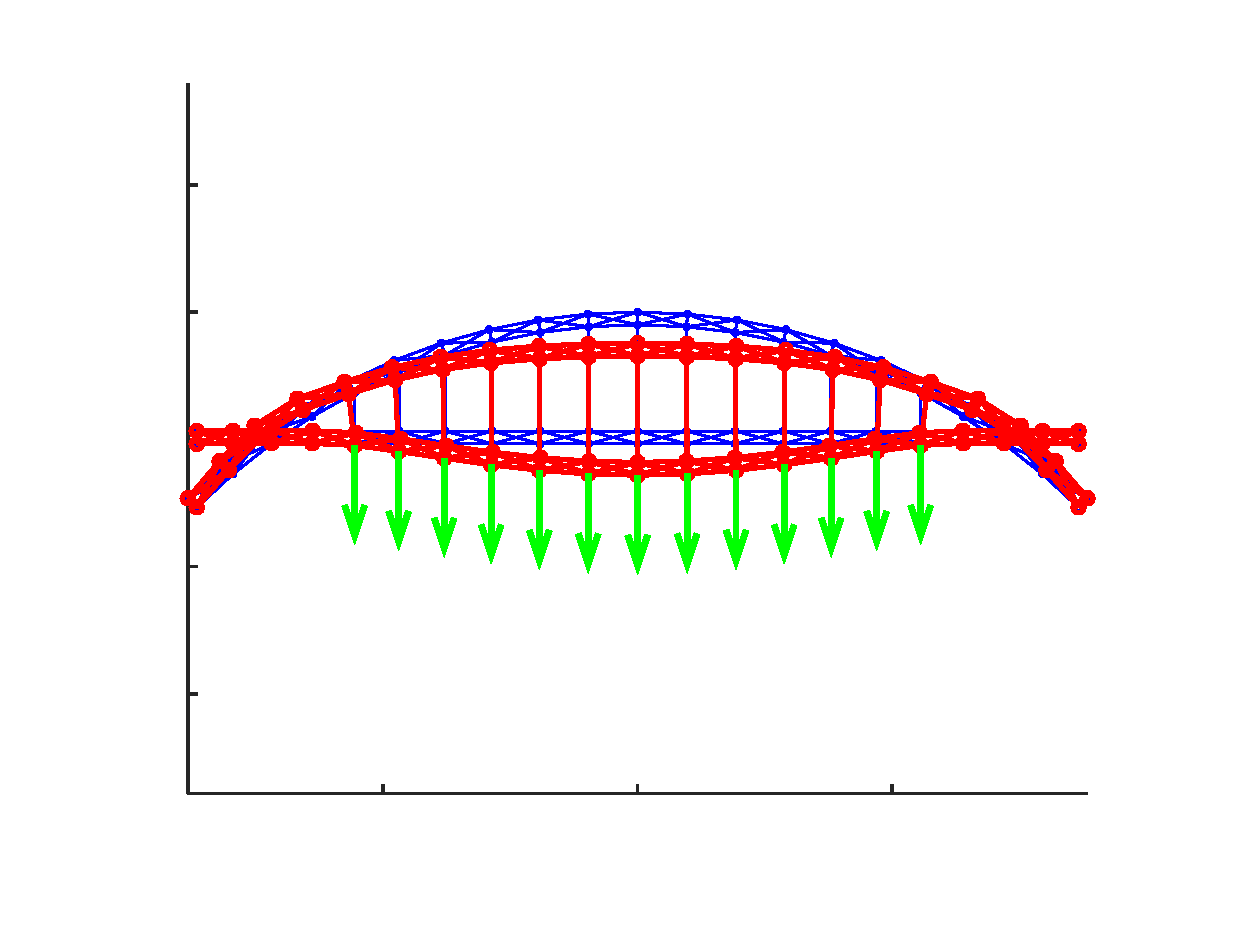
\includegraphics{ArchBridge_deform-inc}
\end{picture}%
\begin{picture}(576,432)(0,0)
\fontsize{22}{0}
\selectfont\put(175.935,54.0045){\makebox(0,0)[t]{\textcolor[rgb]{0.15,0.15,0.15}{{-20}}}}
\fontsize{22}{0}
\selectfont\put(298.08,54.0045){\makebox(0,0)[t]{\textcolor[rgb]{0.15,0.15,0.15}{{0}}}}
\fontsize{22}{0}
\selectfont\put(420.225,54.0045){\makebox(0,0)[t]{\textcolor[rgb]{0.15,0.15,0.15}{{20}}}}
\fontsize{22}{0}
\selectfont\put(77.1587,106.816){\makebox(0,0)[r]{\textcolor[rgb]{0.15,0.15,0.15}{{20}}}}
\fontsize{22}{0}
\selectfont\put(77.1587,167.889){\makebox(0,0)[r]{\textcolor[rgb]{0.15,0.15,0.15}{{30}}}}
\fontsize{22}{0}
\selectfont\put(77.1587,228.961){\makebox(0,0)[r]{\textcolor[rgb]{0.15,0.15,0.15}{{40}}}}
\fontsize{22}{0}
\selectfont\put(77.1587,290.033){\makebox(0,0)[r]{\textcolor[rgb]{0.15,0.15,0.15}{{50}}}}
\fontsize{22}{0}
\selectfont\put(77.1587,351.106){\makebox(0,0)[r]{\textcolor[rgb]{0.15,0.15,0.15}{{60}}}}
\fontsize{22}{0}
\selectfont\put(298.08,27.0046){\makebox(0,0)[t]{\textcolor[rgb]{0.15,0.15,0.15}{{x}}}}
\fontsize{22}{0}
\selectfont\put(45.1586,229.299){\rotatebox{90}{\makebox(0,0)[b]{\textcolor[rgb]{0.15,0.15,0.15}{{y}}}}}
\end{picture}
}
	%	\resizebox{.47\linewidth}{!}{\input{sourcesJPZ/figs/Arch_Bridge}}
	\caption{Geometría de modelo simplificado de puente arco con tablero inferior.}
	\label{fig:arcobridge}
\end{figure}
%

El análisis de elementos como cables o tensores es realizado considerando un comportamiento constitutivo no lineal, tema que se aborda en el siguiente capítulo.





\section{Ejercicios}




%--------------- EJ1 ----------------------------------------------------------------------

\bigskip
\begin{exercise}
	
	Probar la condición de estabilidad para $V$ diferenciable para el caso de $n$ grados de libertad. La prueba es similar a la dada en las notas para un grado de libertad, pero trabajando en varias variables.
	
	$$\text{Estabilidad } \Leftarrow \left. \textbf{H}_V  \right|_{\hat{q}} \text{ es definida positiva.}$$
	
\end{exercise}

%--------------- EJ2 ----------------------------------------------------------------------

\bigskip
\begin{exercise}
	
	Hallar las ecuaciones de equilibrio y determinar la carga crítica $P^C$ para las estructuras dadas en las notas:
	\begin{itemize}
		\item Caso de Punto Límite (Figura~\ref{fig:fig9})
		
		
		\item Caso de Bifurcación Simétrica Inestable (Figura~\ref{fig:fig11})
		\item Caso de Bifurcación Asimétrica (Figura~\ref{fig:fig12})
	\end{itemize}
\end{exercise}

%--------------- EJ3 ----------------------------------------------------------------------

\bigskip
\begin{exercise}
	
	Estudiar mediante el Principio de Mínima Energía Potencial Total las configuraciones de equilibrio del sistema discreto formado por barras rígidas dado en la Figura \ref{fig:Ej3a} y clasifique la estabilidad del mismo.
	
	La unión entre barras rígidas transmite cargas normales, permite deslizamiento lateral sin fricción entre ellas y mantiene las barras paralelas en todo momento.
	En la situación decargada ($P=0$) la estructura se encuentra perfectamente recta ($\theta=0$).
	
	Notar que el sistema se encuentra traccionado. ¿Considera posible una bifurcación o inestabilidad en presencia de tracciones?
	
	\begin{figure}[h!]
		\centering
		\includegraphics[width=.60\linewidth]{Pr2_BifTension}
		\caption{Sistema Discreto Sometido a Tensión}
		\label{fig:Ej3a}
	\end{figure}
	
	Se recomienta ver el video disponible en el siguiente enlace, luego de resuelto el ejercicio:  \href{https://www.youtube.com/watch?v=EKngs1vvcJU\&t=92s}{youtube.com/watch?v=EKngs1vvcJU\&t=92s}.
	
\end{exercise}

%--------------- EJ4 ----------------------------------------------------------------------

\bigskip
\begin{exercise}
	
	Se plantea analizar el pandeo de una versión discreta de una columna inextensible. La misma está formada por tres segmentos rígidos unidos por resortes de giro de constante $k$, tal como se muestra en la Figura \ref{fig:Ej3}. La columna es perfectamente recta en su configuración inicial.
	
	\begin{enumerate}
		\item[i)] Determinar las cargas y modos de deformación correspondientes a las configuraciones de equilibrio inestable de la estructura.
		
		\begin{figure}[h!]
			\centering
			\includegraphics[width=.35\linewidth]{P2_EJ3}
			\caption{Columna con dos resortes de giro}
			\label{fig:Ej3}
		\end{figure}
		
		\item[ii)] Utilice la carga crítica hallada para aproximar la carga crítica de Euler. Se sugiere usar la relación Momento-Curvatura: $M/EI=\theta'$.
		
	\end{enumerate}
	
\end{exercise}

%--------------- EJ5 ----------------------------------------------------------------------

\bigskip
\begin{exercise}
	
	Hallar las ecuaciones de equilibrio, los puntos críticos y estudiar la estabilidad de las curvas de carga-desplazamiento para el caso de Bifurcación Simétrica Inestable (Figura 2.4 de las notas) con una imperfección angular inicial $\epsilon$.
\end{exercise}

%--------------- EJ6 ----------------------------------------------------------------------


\bigskip
\begin{exercise}
	
	Se define la configuración de la columna inextensible de largo ($L$) mediante la función $w:[0,L]\rightarrow \mathbb{R}$. Es decir, $w(x)$ da el desplazamiento lateral de la columna respecto de la posición vertical recta.
	
	Las condiciones de borde de la columna son:
	
	\begin{itemize}
		\item Apoyo en los extremos: $w(0)=0$ y $w(L)=0$.
		\item Momento Nulo en los extremos: $w''(0)=0$ y $w''(L)=0$.
	\end{itemize}
	
	Dadas las siguientes expresiones para la energía elástica interna ($U$) de flexión y el descenso ($\Delta$) del extremo superior de la columna:
	
	\begin{equation}
		U[w] = \int_{0}^{L} \frac{EI}{2}\frac{{w''(s)}^2}{1-w'(s)^2} ds \simeq \frac{1}{2}\int_{0}^{L} EI{w''(x)}^2 dx
	\end{equation}
	
	\begin{equation}
		\Delta[w] = \int_{0}^{L} 1-\sqrt{1-w'(s)^2} ds \simeq \int_{0}^{L} \frac{w'(x)^2}{2} dx
	\end{equation}
	
	Se pide:
	
	\begin{enumerate}
		\item[i)] Justifique las expresiones dadas para la energía elástica interna ($U$) y el descenso del extremo superior de la columna ($\Delta$).
		
		\item[ii)] Deducir mediante el Principio de Mínima Energía Potencial la E.D.O. que gobierna el equilibrio de la columnas inextensibles en compresión.
		
		\item[iii)] Transformar el problema de minimización continuo en uno discreto al proponer una deformada de la forma $\hat{w}(x)=qx(x-L)$. ¿La deformada verifica todas las condiciones de borde? Estime la carga crítica a partir de dicha $\hat{w}(x)$.
	\end{enumerate}
	
	
\end{exercise}


%--------------- EJ6b ----------------------------------------------------------------------

\bigskip
\begin{exercise}
	
	Se determinará, mediante el Principio de Mínima Energía Potencial Total, una aproximación de la carga crítica del \textit{Roorda Frame} dado en la Figura \ref{fig:Ej6b}.
	
	\begin{figure}[h!]
		\centering
		\includegraphics[width=.4\linewidth]{RoordaFrame}
		\caption{Estructura Tipo \textit{Roorda Frame}}
		\label{fig:Ej6b}
	\end{figure}
	
	Las barras son inextensibles, de acero ($E=210000$ MPa) y tienen sección rectangular ($a=10 \text{ mm}$ y $b=50\text{ mm}$). Las mismas experimentan flexión según su inercia débil.
	
	Utilizar funciones cúbicas para expresar la deformación lateral $w(x)$ de cada barra. En particular, llamado $\theta_A$ y $\theta_B$ a los giros en los extremos $A$ y $B$ respectivamente, se sugiere la expresión:
	
	$$w(x) = \theta_A L \frac{x}{L}\left(1-\frac{x}{L}\right)^2 - \theta_B L \left(\frac{x}{L}\right)^2 \left( 1-\frac{x}{L} \right)$$
	
	Se pide:
	
	\begin{enumerate}
		\item[i)] Estimar la carga crítica y el modo asociado usando el PMEPT y las funciones de deflexión lateral sugeridas.
		
		\item[ii)] Calcular mediante el ábaco de Jackson \& Mooreland la carga crítica de la estructura considerada. Compare contra la carga crítica estimada en i).
		
		\item[iii)] \textquestiondown Qué relación opina que existe entre la estimación de carga crítica realizada y el Método de Elementos Finitos? Si lo entiende necesario, compare el resultado obtenido contra cálculos usando algún \textit{software} comercial (o académico) variando la cantidad de elementos por barra.
	\end{enumerate}
	
	
\end{exercise}

%%%%%%%%%%%%%%%%%%%%%%%%%%%%%%%%%%%%%%%%%%%%%%%%%%%%%%%%%%%%%
%\pagebreak


%\begin{exercise}
	%	
	%	Mostrar que el PTV para una partícula implica el equilibrio dado por la Ley de Newton. Es decir:
	%	
	%	$$\delta W_{ext}=0  \quad \forall \delta u \quad  \Longrightarrow \quad \sum_i \textbf{f}_i = 0$$
	%
	%\end{exercise}
%
%
%\begin{exercise}
	%	
	%	Se pide calcular el descenso de una viga simplemente apoyada con carga uniforme utilizando el PTV. Se desprecia la deformación por cortante, se asumen pequeños desplazamientos y material elástico lineal (Módulo de Elasticidad: $E$ y Segundo Momento de Inercia: $I_y$).
	%	
	%	\begin{enumerate}
		%		\item[1)] Realizar el cálculo asumiendo una deformada expresada como serie trigonométrica: $w(x)=\sum_{i=0}^N q_i \sin((2i+1)\pi x/L)$. Estimar el descenso central usando 1,2 y 3 términos de la serie.
		%		
		%		\item[2)] Realizar el cálculo asumiendo una deformada dada por un polinomio de orden 4. El cálculo es más simple si se elije aquel polinomio que verifica todas las condiciones de contorno (desplazamientos y momentos nulos). Analizar los resultados.
		%	\end{enumerate}
	%	
	%\end{exercise}
%
%
%%--------------- EJ8 ----------------------------------------------------------------------
%\begin{exercise}
	%	
	%	En el ejemplo de la barra rígida simplemente apoyada, visto en la Sección 2.2.2 de las notas, usar el PTV para determinar:
	%	\begin{itemize}
		%		\item Las tres reacciones de los apoyos usando solamente un desplazamiento virtual (movimiento de cuerpo rígido).
		%		
		%		\item El momento flector resistido por la barra rígida en el centro del vano.
		%	\end{itemize}
	%\end{exercise}



\begin{exercise}
	
	Repetir el Ejercicio 5 usando el PTV para hallar la ecuación de equilibrio de la estructura. Verificar que se obtiene la misma ecuación de equilibrio que usando el Principio de Mínima Energía Potencial.
\end{exercise}


\bigskip


\begin{exercise}
	
	En este ejercicio se pide verificar la validez de las siguientes equivalencias dadas en la Sección 2.3 de las notas del curso.
	\bigskip
	
	\textit{Equivalencias entre medidas de deformación:}
	
	\begin{itemize}
		\item $\varepsilon_G = \varepsilon_E(1+\varepsilon_E/2)$
		\item $\varepsilon_L = \ln(1+\varepsilon_E)$
		\item $\varepsilon_L = \frac{1}{2}\ln(1+2\varepsilon_G)$
	\end{itemize}
	
	\textit{Equivalencias entre medidas de tensión:}
	
	\begin{itemize}
		\item $\sigma_E = \sigma A_n / A_o$
		\item $\sigma_G = \sigma A_n l_o / (A_o l_n)$
	\end{itemize}
	
\end{exercise}


\bigskip


\begin{exercise}

Considere una viga simplemente apoyada sometida al peso de un fluido como se muestra en la \autoref{fig:ejPonding}. El recinto del fluido es llenado de forma tal que la cota es mantenida en $h$, incluso cuando la viga es deformada. %
%
La viga tiene rigidez flexional $EI$, largo $\ell$ y ancho $b$.

\begin{figure}[htb]
	\centering
\includegraphics[width=0.95\textwidth]{ejPonding}
\caption{Diagrama de viga con carga de fluido.}
\label{fig:ejPonding}
\end{figure}


Se considera que la viga tiene una rigidez tal que es razonable considerar una elástica con pequeños giros, sin embargo, se debe considerar el desplazamiento $w(x)$ en el cálculo de la presión. Como aproximación de la solución se admite válido utilizar funciones sinusoidales de la forma:
$$
w(x)=A\sin\left( \pi \frac{x}{\ell} \right).
$$

\textbf{Se pide:}

	\begin{enumerate}
	\item[i)] Deducir las expresiones del trabajo virtual de las fuerzas internas y trabajo virtual de las fuerzas externas en función de $w$ y $\delta w$.
	\item[ii)] Determinar el descenso máximo de la viga utilizando el PTV con la deformada sinusoidal.
	\item[iii)] Escribir el descenso de la parte anterior como el producto del descenso de
	primer orden (i.e. lineal y asumiendo deformada sinusoidal) y un factor a determinar. Estudiar dicho factor.
	\end{enumerate}
\end{exercise}

%\bigskip
%
%
%%--------------- EJ11 ----------------------------------------------------------------------
%
%\begin{exercise}
%	
%	Utilizar el código dado en la Sección 2.3 de las notas del curso para estudiar cómo al cambiar $z$ mejora la aproximación de las curvas de carga desplazamiento obtenidas para las distintas medidas de deformación no-lineal bajo la hipótesis de módulo de elasticidad constante ($E$) para todos los casos. 
%	
%	Identificar para qué valor de deformación unitaria la aproximación entre todas las medidas de deformación pasa a ser razonable en el ejemplo visto.
%\end{exercise}
%
%%--------------- EJ12 ----------------------------------------------------------------------
%
%%\bigskip
%%\begin{exercise}
%%	\textbf{(Ejercicio Posgrado)} 
%%	
%%	En este ejercicio se introduce el tensor de deformaciones de Green y se verifica la invarianza del mismo frente a rotaciones de cuerpo rígido del sólido bajo estudio.
%%	
%%	Trabajando en un conjunto de ejes cartesianos fijos, un punto $P$ del sólido en su configuración inicial es dado por $\bfx_0$ y el mismo punto en la configuración deformada está dado por $\bfx_t=\chi(x_0,t)$.
%%	
%%	El desplazamiento del punto P se define como: $\bfu_t = \bfx_t - \bfx_0$. Y un diferencial de posición en la configuración deformada se relaciona a uno en la configuración inicial mediante:
%%	
%%	$$\dif \bfx_t = \dfrac{\partial \bfx_t}{\partial \bfx_0} \dif \bfx_0$$
%%	
%%	En base a lo anterior se definen el gradiente de deformaciones como: $\bfF = \dfrac{\partial \bfx_t}{\partial \bfx_0}$ y la matriz de derivadas del desplazamiento como: $\bfD = \dfrac{\partial \bfu_t}{\partial \bfx_0}$.
%%	
%%	Se pide:
%%	
%%	\begin{enumerate}
%%		\item[i)] Mostrar que: $\bfD = \bfF - \bfI$
%%		\item[ii)] Deducir el tensor de deformaciones de Green ($\bfE$) escribiéndolo tanto en función de $\bfF$ como de $\bfD$. 
%%		
%%		\textbf{Sugerencia: }Partir de: $\dif{\bfx_t}^T\dif\bfx_t-\dif\bfx_0^T\dif\bfx_0$ y recordar la definición de Deformación de Green uni-axial vista en la Sección 2.3.3 de las notas del curso: $l_t^2 - l_0^2 = 2 l_0 \varepsilon_G l_0$.
%%		
%%		\item[iii)] Asumir que el sólido es sometido a una deformación tal que la posición de un punto $P$ cualquiera en el estado deformado corresponde a una rotación rígida respecto del origen de coordenadas del punto $P$ en la configuración inicial ($\bfx_t = \bfR \bfx_0$). 
%%		
%%		Evaluar el tensor de deformación de Green ($\bfE$) para esta deformación asumiendo una rotación en el plano $x-y$. Evaluar también el tensor de deformaciones infinitesimal visto en elasticidad lineal. Comparar ambos resultados y comentar sobre el efecto de movimientos de cuerpo rígido sobre los mismos.
%%	\end{enumerate}
%%\end{exercise}
%
%
%\bigskip
%
%\begin{exercise}
%	
%	Considerando la Sección~2.4 de las notas del curso:
%	\begin{enumerate}
%		\item[i)] Demostrar que $\textbf{b}_1$ es igual a $\textbf{b}_L$
%		\item[ii)] Demostrar que $\textbf{K}_{T1}$ es igual a $\textbf{K}_L$.
%		\item[iii)] Demostrar que para una barra dada $e$, las fuerzas internas $\bff^e_{int}$ de cada nodo son colineales con la barra. 
%	\end{enumerate}
%\end{exercise}
%
%
%\bigskip
%
%
%\begin{exercise}
%	
%	En el curso, al igual que en el ejercicio siguiente, se asume que el gradiente de una función $g$ real escalar es un vector fila donde la entrada $i$-ésima es la derivada parcial $\partial g(\bfx) / \partial x_i$ y que el gradiente de una función vectorial $f(\bfx):\bbR^n \rightarrow \bbR^m$ (formada por $m$ funciones escalares $f_j (\bfx)$) es una matriz donde la entrada de la fila $p$ y la columna $q$ está dada por:
%	\begin{equation} 
%		\left( \frac{\partial f}{\partial \bfx}  \right)_{pq} = \frac{\partial f_p}{ \partial x_q}
%	\end{equation} 
%	
%	\begin{enumerate}
%		\item[i)]
%		Sean $\bfx$, $\bfb$ y $\bff(\bfx)$ son vectores columna de $n$ entradas, $\bfA$ una matriz de tamaño $n\times n$ (no necesariamente simétrica) y $a$, $g(\bfx)$ son escalares, demostrar las siguientes identidades:
%		
%		\begin{enumerate}
%			\item $\dfrac{\partial \bfx^T \bfb}{\partial \bfx} = \bfb^T$
%			\item $\dfrac{\partial \bfb^T \bfx}{\partial \bfx} = \bfb^T$
%			\item $\dfrac{\partial \bfA \bfx}{\partial \bfx} = \bfA$
%			\item $\dfrac{\partial \bfx^T \bfA \bfx }{\partial \bfx} = \bfx^T \bfA  + \bfx^T \bfA^T $
%			\item $\dfrac{\partial \| \bfx \|^2 }{\partial \bfx} = 2 \bfx^T$
%			\item $\dfrac{\partial a \bfx }{\partial \bfx} = a \bfI$  \quad (siendo $\bfI$ la matriz identidad)
%			\item $\dfrac{\partial g(\bfx)\bff(\bfx)}{\partial \bfx} = \bff(\bfx)\dfrac{\partial g(\bfx)}{\partial \bfx}+g(\bfx)\dfrac{\partial \bff(\bfx)}{\partial \bfx} \quad \text{con}\quad g:\mathbb{R}^n\rightarrow \mathbb{R} \quad \text{y}\quad \bff:\mathbb{R}^n\rightarrow \mathbb{R}^n$
%		\end{enumerate}
%		
%		\item[ii)] Usando las relaciones anteriores mostrar que se cumplen las siguientes relaciones vistas en el Capítulo 2 de las notas:
%		
%		\begin{itemize}
%			\item Dado $\varepsilon(\bfu^e)=({(\bfx^e)}^T\bfG^e\bfu^e+\frac{1}{2}{(\bfu^e)}^T\bfG^e\bfu^e)/l_0^2$ se cumple: 
%			
%			$$\dfrac{\partial \varepsilon(\bfu^e)}{\partial \bfu^e} = \frac{1}{l_0^2}({(\bfx^e)}^T\bfG^e + {(\bfu^e)}^T\bfG^e)$$
%			
%			\item Dado $\bff^e_{int}(\bfu^e)=A_0\int_{l_0}\sigma(\bfu^e) \bfb^e(\bfu)^T dx$ se cumple:
%			
%			$$ \dfrac{\partial \bff^e_{int}(\bfu^e)}{\partial \bfu^e} = A_0\int_{l_0} \bfb^e(\bfu^e)^T \dfrac{\partial \sigma(\bfu^e)}{\partial \bfu^e}+ \sigma(\bfu^e)\dfrac{\partial \bfb^e(\bfu^e)^T}{\partial \bfu^e} dx  $$
%			
%		\end{itemize}
%		
%	\end{enumerate}
%\end{exercise}
%
%
%\bigskip
%
%
%\begin{exercise}
%	
%	A través de modificaciones del Código 2.3 se pide: 
%	\begin{enumerate}
%		\item[i)] Resolver el problema de la Sección 3.1 del artículo de Li \& Khandelwal. Utilizar los ángulos considerados en el artículo (65$^\circ$) y también $85^\circ$. Comparar los resultados para los distintos ángulos y verificar usando el NSA.
%		
%		\item[ii)] Establecer si existe relación entre el punto límite de la carga fuerza-desplazamiento y el punto de pérdida de rigidez del elemento de barra de Green dado por la medida de deformación y la relación constitutiva. %
%		
%		\item[iii)] Modificar el código para tomar en cuenta el criterio de parada en fuerzas residuales en lugar de convergencia en desplazamientos. %
%		%
%		Resolver el problema de Von Mises ingresando las fuerzas externas en diferentes unidades. Analizar si hay cambios en la cantidad de iteraciones requeridas por el método para encontrar la solución.
%		
%		\item[iv)] Demostrar que si existen resortes lineales en los nodos, la matriz de constantes elásticas de resortes $\textbf{K}_S$ puede ser sumada a la matriz $\textbf{K}_T$ y considerada para calcular el término adicional de fuerzas internas.
%		
%		\item[v)] Modificar el código para resolver considerando carga incremental y un resorte de constante $k$ variable. Reproducir el comportamiento mostrado en la Figura 1.2 de la Sección 1.2 del libro de Crisfield volumen 1.
%	\end{enumerate}
%\end{exercise}
%
%\bigskip
%
%
%%
%%\begin{exercise}
%%	
%%	Utilizando el código NSA y las equivalencias entre reticulados y vigas, obtener las curvas fuerza-desplazamiento post-críticas de:
%%	\begin{enumerate}
%%		\item[i)] Una barra bi-articulada con carga axial de compresión $P$ con excentricidad en dicha carga igual a $e$.
%%		\item[ii)] La estructura considerada en el Ejercicio 7 del Práctico 2a: \textit{Roorda Frame}. Reproducir el comportamiento mostrado en la Figura 4.7 del libro \textit{Elastic Stability Phenomena} de Thompson y Hunt considerando que la carga tiene una excentricidad $e$ hacia la derecha o hacia la izquierda. Utilizar el archivo input disponible en el sitio EVA.
%%	\end{enumerate}
%%\end{exercise}
%%
%
%\begin{exercise}
%	
%	Se considera la estructura de barras articuladas que se muestra en la Figura \ref{fig:EjLBA}. La estructura es perfecta, es decir completamente horizontal cuando $P=0$.
%	
%	\begin{figure}[htb]
%		\centering
%		\includegraphics[width=1\linewidth]{EjercicioLBA}
%		\caption{Estructura Perfecta (Horizontal cuando $P=0$)}
%		\label{fig:EjLBA}
%	\end{figure}
%	
%	Todas las barras tienen largo $L$, área $A$ y módulo de elasticidad $E$. Ambos resortes tienen constante $k$.
%	
%	Se pide:
%	
%	\begin{enumerate}
%		\item[i)] Determinar la carga crítica de pandeo y su modo asociado mediante el Principio de Mínima Energía Potencial Total. Asumir para esta parte que las barras son infinitamente rígidas a directa.
%		
%		\item[ii)] Determinar, mediante cálculos manuales, la carga crítica de pandeo y modo asociado mediante un análisis \textit{LBA} usando barras de Green. Comparar esta solución contra la obtenida en el ítem anterior.
%		
%		\textbf{Sugerencias:} 
%		
%		\begin{itemize}
%			\item Ensamblar solamente los términos de las matrices correspondientes a los grados de libertad libres (matriz global 5x5). 
%			
%			\item Reordenar filas y columnas de las matrices previo al cálculo del determinante a fin de desacoplar los modos de pandeo buscados.
%		\end{itemize}
%		
%		\item[iii)] Modelar la estructura en ONSAS usando los parámetros: $L=1000$, $E=2.1\times 10^5$, $A=100$ y $K=2100$. Verificar la carga crítica y modo asociado determinados en el ítem anterior. Incorporar una imperfección y analizar la estructura mediante \textit{Arc-Length}. Clasificar la estabilidad post-critica de la estructura.
%		
%	\end{enumerate}
%	
%\end{exercise}
%
%\begin{exercise}
%
%	Utilizando los modelos de ONSAS desarrollados en el Ejercicio 7 de este práctico, determinar las cargas y modos de pandeo mediante \textit{LBA} y compararlos contra los valores teóricos de pandeo (para \textit{Roorda Frame} utilizar resultados del Ejercicio 7 del Práctico 2a).
%\end{exercise}
%
%
%
%
%

